\documentclass{bmvc2k}

\bmvcreviewcopy{---}

\title{CFFM-Net: Reliability-Gated Mamba Fusion of Visible and Thermal Images}
\addauthor{Anonymous}{anonymous@example.com}{1}
\addinstitution{Anonymous Institution}
\runninghead{Anonymous}{CFFM-Net}

\usepackage{amsmath,mathtools}
\usepackage{booktabs,graphicx}
\usepackage{xurl}
\DeclareMathOperator{\softplus}{softplus}
\newcommand{\Fv}{F^{v}}
\newcommand{\Ft}{F^{\theta}}
\newcommand{\rv}{r^{v}}
\newcommand{\rt}{r^{\theta}}
% generated by tools/collect_numbers.py; do not edit by hand
% results: LLVIP CFFM-Net v1 seed 0, percent
\newcommand{\resLlvipCffmVoneSeedZeroMap}{62.9}
\newcommand{\resLlvipCffmVoneSeedZeroMapFifty}{95.8}
\newcommand{\resLlvipCffmVoneSeedZeroPrecision}{96.2}
\newcommand{\resLlvipCffmVoneSeedZeroRecall}{90.7}
\newcommand{\resLlvipCffmVoneSeedZeroApSmall}{8.9}
\newcommand{\resLlvipCffmVoneSeedZeroApMedium}{62.7}
\newcommand{\resLlvipCffmVoneSeedZeroApLarge}{64.9}
\newcommand{\resLlvipCffmVoneSeedZeroApBandSmall}{8.9}
% results: LLVIP v1, gated conv seed 0, percent
\newcommand{\resLlvipCffmVoneGconvSeedZeroMap}{62.8}
\newcommand{\resLlvipCffmVoneGconvSeedZeroMapFifty}{96.0}
\newcommand{\resLlvipCffmVoneGconvSeedZeroPrecision}{96.3}
\newcommand{\resLlvipCffmVoneGconvSeedZeroRecall}{90.8}
\newcommand{\resLlvipCffmVoneGconvSeedZeroApSmall}{6.1}
\newcommand{\resLlvipCffmVoneGconvSeedZeroApMedium}{62.6}
\newcommand{\resLlvipCffmVoneGconvSeedZeroApLarge}{65.1}
\newcommand{\resLlvipCffmVoneGconvSeedZeroApBandSmall}{6.1}
% results: LLVIP v1, no gate seed 0, percent
\newcommand{\resLlvipCffmVoneNogateSeedZeroMap}{62.6}
\newcommand{\resLlvipCffmVoneNogateSeedZeroMapFifty}{96.0}
\newcommand{\resLlvipCffmVoneNogateSeedZeroPrecision}{96.2}
\newcommand{\resLlvipCffmVoneNogateSeedZeroRecall}{89.7}
\newcommand{\resLlvipCffmVoneNogateSeedZeroApSmall}{6.4}
\newcommand{\resLlvipCffmVoneNogateSeedZeroApMedium}{62.3}
\newcommand{\resLlvipCffmVoneNogateSeedZeroApLarge}{66.0}
\newcommand{\resLlvipCffmVoneNogateSeedZeroApBandSmall}{6.5}
% results: LLVIP v1, no P2 head seed 0, percent
\newcommand{\resLlvipCffmVoneNoptwoSeedZeroMap}{63.5}
\newcommand{\resLlvipCffmVoneNoptwoSeedZeroMapFifty}{96.0}
\newcommand{\resLlvipCffmVoneNoptwoSeedZeroPrecision}{95.3}
\newcommand{\resLlvipCffmVoneNoptwoSeedZeroRecall}{90.1}
\newcommand{\resLlvipCffmVoneNoptwoSeedZeroApSmall}{7.5}
\newcommand{\resLlvipCffmVoneNoptwoSeedZeroApMedium}{63.3}
\newcommand{\resLlvipCffmVoneNoptwoSeedZeroApLarge}{64.9}
\newcommand{\resLlvipCffmVoneNoptwoSeedZeroApBandSmall}{7.5}
% results: LLVIP CFFM-Net v3 seed 0, percent
\newcommand{\resLlvipCffmVthreeSeedZeroMap}{64.0}
\newcommand{\resLlvipCffmVthreeSeedZeroMapFifty}{95.8}
\newcommand{\resLlvipCffmVthreeSeedZeroPrecision}{95.6}
\newcommand{\resLlvipCffmVthreeSeedZeroRecall}{88.6}
\newcommand{\resLlvipCffmVthreeSeedZeroApSmall}{6.5}
\newcommand{\resLlvipCffmVthreeSeedZeroApMedium}{63.2}
\newcommand{\resLlvipCffmVthreeSeedZeroApLarge}{68.8}
\newcommand{\resLlvipCffmVthreeSeedZeroApBandSmall}{6.5}
% results: LLVIP v3, no reliability branch seed 0, percent
\newcommand{\resLlvipCffmVthreeNorelSeedZeroMap}{67.2}
\newcommand{\resLlvipCffmVthreeNorelSeedZeroMapFifty}{96.6}
\newcommand{\resLlvipCffmVthreeNorelSeedZeroPrecision}{96.0}
\newcommand{\resLlvipCffmVthreeNorelSeedZeroRecall}{91.2}
\newcommand{\resLlvipCffmVthreeNorelSeedZeroApSmall}{10.1}
\newcommand{\resLlvipCffmVthreeNorelSeedZeroApMedium}{66.5}
\newcommand{\resLlvipCffmVthreeNorelSeedZeroApLarge}{71.0}
\newcommand{\resLlvipCffmVthreeNorelSeedZeroApBandSmall}{10.1}
% results: LLVIP CFFM-Net v2 seed 0, percent
\newcommand{\resLlvipCffmVtwoSeedZeroMap}{65.6}
\newcommand{\resLlvipCffmVtwoSeedZeroMapFifty}{97.0}
\newcommand{\resLlvipCffmVtwoSeedZeroPrecision}{96.4}
\newcommand{\resLlvipCffmVtwoSeedZeroRecall}{92.4}
\newcommand{\resLlvipCffmVtwoSeedZeroApSmall}{8.2}
\newcommand{\resLlvipCffmVtwoSeedZeroApMedium}{65.5}
\newcommand{\resLlvipCffmVtwoSeedZeroApLarge}{66.8}
\newcommand{\resLlvipCffmVtwoSeedZeroApBandSmall}{8.2}
% results: LLVIP CFFM-Net v2 seed 1, percent
\newcommand{\resLlvipCffmVtwoSeedOneMap}{66.0}
\newcommand{\resLlvipCffmVtwoSeedOneMapFifty}{96.6}
\newcommand{\resLlvipCffmVtwoSeedOnePrecision}{97.1}
\newcommand{\resLlvipCffmVtwoSeedOneRecall}{91.2}
\newcommand{\resLlvipCffmVtwoSeedOneApSmall}{9.0}
\newcommand{\resLlvipCffmVtwoSeedOneApMedium}{65.5}
\newcommand{\resLlvipCffmVtwoSeedOneApLarge}{68.7}
\newcommand{\resLlvipCffmVtwoSeedOneApBandSmall}{9.0}
% results: LLVIP CFFM-Net v2 seed 2, percent
\newcommand{\resLlvipCffmVtwoSeedTwoMap}{67.1}
\newcommand{\resLlvipCffmVtwoSeedTwoMapFifty}{97.2}
\newcommand{\resLlvipCffmVtwoSeedTwoPrecision}{96.4}
\newcommand{\resLlvipCffmVtwoSeedTwoRecall}{92.4}
\newcommand{\resLlvipCffmVtwoSeedTwoApSmall}{10.2}
\newcommand{\resLlvipCffmVtwoSeedTwoApMedium}{66.5}
\newcommand{\resLlvipCffmVtwoSeedTwoApLarge}{70.5}
\newcommand{\resLlvipCffmVtwoSeedTwoApBandSmall}{10.2}
% results: LLVIP Concat, fault training seed 0, percent
\newcommand{\resLlvipConcatFtSeedZeroMap}{66.4}
\newcommand{\resLlvipConcatFtSeedZeroMapFifty}{96.5}
\newcommand{\resLlvipConcatFtSeedZeroPrecision}{96.1}
\newcommand{\resLlvipConcatFtSeedZeroRecall}{91.9}
\newcommand{\resLlvipConcatFtSeedZeroApSmall}{8.0}
\newcommand{\resLlvipConcatFtSeedZeroApMedium}{65.7}
\newcommand{\resLlvipConcatFtSeedZeroApLarge}{70.4}
\newcommand{\resLlvipConcatFtSeedZeroApBandSmall}{8.0}
% results: LLVIP Concat, modality dropout seed 0, percent
\newcommand{\resLlvipConcatMdSeedZeroMap}{64.8}
\newcommand{\resLlvipConcatMdSeedZeroMapFifty}{97.2}
\newcommand{\resLlvipConcatMdSeedZeroPrecision}{96.8}
\newcommand{\resLlvipConcatMdSeedZeroRecall}{91.7}
\newcommand{\resLlvipConcatMdSeedZeroApSmall}{8.0}
\newcommand{\resLlvipConcatMdSeedZeroApMedium}{64.7}
\newcommand{\resLlvipConcatMdSeedZeroApLarge}{66.1}
\newcommand{\resLlvipConcatMdSeedZeroApBandSmall}{8.0}
% results: LLVIP Concat, modality dropout seed 1, percent
\newcommand{\resLlvipConcatMdSeedOneMap}{66.3}
\newcommand{\resLlvipConcatMdSeedOneMapFifty}{96.6}
\newcommand{\resLlvipConcatMdSeedOnePrecision}{97.0}
\newcommand{\resLlvipConcatMdSeedOneRecall}{91.7}
\newcommand{\resLlvipConcatMdSeedOneApSmall}{9.6}
\newcommand{\resLlvipConcatMdSeedOneApMedium}{65.8}
\newcommand{\resLlvipConcatMdSeedOneApLarge}{69.3}
\newcommand{\resLlvipConcatMdSeedOneApBandSmall}{9.6}
% results: LLVIP Concat, modality dropout seed 2, percent
\newcommand{\resLlvipConcatMdSeedTwoMap}{65.2}
\newcommand{\resLlvipConcatMdSeedTwoMapFifty}{96.6}
\newcommand{\resLlvipConcatMdSeedTwoPrecision}{96.7}
\newcommand{\resLlvipConcatMdSeedTwoRecall}{90.6}
\newcommand{\resLlvipConcatMdSeedTwoApSmall}{11.0}
\newcommand{\resLlvipConcatMdSeedTwoApMedium}{64.6}
\newcommand{\resLlvipConcatMdSeedTwoApLarge}{68.3}
\newcommand{\resLlvipConcatMdSeedTwoApBandSmall}{11.0}
% results: LLVIP Two-stream concat seed 0, percent
\newcommand{\resLlvipConcatPlainSeedZeroMap}{64.9}
\newcommand{\resLlvipConcatPlainSeedZeroMapFifty}{96.8}
\newcommand{\resLlvipConcatPlainSeedZeroPrecision}{96.2}
\newcommand{\resLlvipConcatPlainSeedZeroRecall}{91.4}
\newcommand{\resLlvipConcatPlainSeedZeroApSmall}{12.7}
\newcommand{\resLlvipConcatPlainSeedZeroApMedium}{64.8}
\newcommand{\resLlvipConcatPlainSeedZeroApLarge}{65.6}
\newcommand{\resLlvipConcatPlainSeedZeroApBandSmall}{12.8}
% results: LLVIP Concat + P2 head seed 0, percent
\newcommand{\resLlvipConcatPtwoSeedZeroMap}{63.2}
\newcommand{\resLlvipConcatPtwoSeedZeroMapFifty}{96.2}
\newcommand{\resLlvipConcatPtwoSeedZeroPrecision}{95.7}
\newcommand{\resLlvipConcatPtwoSeedZeroRecall}{90.5}
\newcommand{\resLlvipConcatPtwoSeedZeroApSmall}{5.6}
\newcommand{\resLlvipConcatPtwoSeedZeroApMedium}{62.9}
\newcommand{\resLlvipConcatPtwoSeedZeroApLarge}{65.9}
\newcommand{\resLlvipConcatPtwoSeedZeroApBandSmall}{5.6}
% results: LLVIP YOLO26-n thermal seed 0, percent
\newcommand{\resLlvipYoloThmSeedZeroMap}{64.1}
\newcommand{\resLlvipYoloThmSeedZeroMapFifty}{96.2}
\newcommand{\resLlvipYoloThmSeedZeroPrecision}{95.7}
\newcommand{\resLlvipYoloThmSeedZeroRecall}{91.6}
\newcommand{\resLlvipYoloThmSeedZeroApSmall}{6.4}
\newcommand{\resLlvipYoloThmSeedZeroApMedium}{63.5}
\newcommand{\resLlvipYoloThmSeedZeroApLarge}{67.4}
\newcommand{\resLlvipYoloThmSeedZeroApBandSmall}{6.4}
% results: LLVIP YOLO26-n visible seed 0, percent
\newcommand{\resLlvipYoloVisSeedZeroMap}{52.0}
\newcommand{\resLlvipYoloVisSeedZeroMapFifty}{90.0}
\newcommand{\resLlvipYoloVisSeedZeroPrecision}{92.4}
\newcommand{\resLlvipYoloVisSeedZeroRecall}{83.4}
\newcommand{\resLlvipYoloVisSeedZeroApSmall}{9.3}
\newcommand{\resLlvipYoloVisSeedZeroApMedium}{50.6}
\newcommand{\resLlvipYoloVisSeedZeroApLarge}{59.1}
\newcommand{\resLlvipYoloVisSeedZeroApBandSmall}{9.3}
% results: M3FD CFFM-Net v1 seed 0, percent
\newcommand{\resMfdCffmVoneSeedZeroMap}{47.9}
\newcommand{\resMfdCffmVoneSeedZeroMapFifty}{77.3}
\newcommand{\resMfdCffmVoneSeedZeroPrecision}{81.1}
\newcommand{\resMfdCffmVoneSeedZeroRecall}{70.3}
\newcommand{\resMfdCffmVoneSeedZeroApSmall}{29.7}
\newcommand{\resMfdCffmVoneSeedZeroApMedium}{59.0}
\newcommand{\resMfdCffmVoneSeedZeroApLarge}{80.2}
\newcommand{\resMfdCffmVoneSeedZeroApBandVeryTiny}{5.9}
\newcommand{\resMfdCffmVoneSeedZeroApBandTiny}{19.0}
\newcommand{\resMfdCffmVoneSeedZeroApBandSmall}{42.8}
% results: M3FD CFFM-Net v3 seed 0, percent
\newcommand{\resMfdCffmVthreeSeedZeroMap}{51.9}
\newcommand{\resMfdCffmVthreeSeedZeroMapFifty}{79.7}
\newcommand{\resMfdCffmVthreeSeedZeroPrecision}{85.4}
\newcommand{\resMfdCffmVthreeSeedZeroRecall}{72.4}
\newcommand{\resMfdCffmVthreeSeedZeroApSmall}{32.0}
\newcommand{\resMfdCffmVthreeSeedZeroApMedium}{66.2}
\newcommand{\resMfdCffmVthreeSeedZeroApLarge}{86.8}
\newcommand{\resMfdCffmVthreeSeedZeroApBandVeryTiny}{5.6}
\newcommand{\resMfdCffmVthreeSeedZeroApBandTiny}{21.9}
\newcommand{\resMfdCffmVthreeSeedZeroApBandSmall}{45.4}
% results: M3FD v3, no reliability branch seed 0, percent
\newcommand{\resMfdCffmVthreeNorelSeedZeroMap}{53.3}
\newcommand{\resMfdCffmVthreeNorelSeedZeroMapFifty}{81.8}
\newcommand{\resMfdCffmVthreeNorelSeedZeroPrecision}{87.5}
\newcommand{\resMfdCffmVthreeNorelSeedZeroRecall}{74.8}
\newcommand{\resMfdCffmVthreeNorelSeedZeroApSmall}{34.8}
\newcommand{\resMfdCffmVthreeNorelSeedZeroApMedium}{66.5}
\newcommand{\resMfdCffmVthreeNorelSeedZeroApLarge}{86.6}
\newcommand{\resMfdCffmVthreeNorelSeedZeroApBandVeryTiny}{6.5}
\newcommand{\resMfdCffmVthreeNorelSeedZeroApBandTiny}{25.0}
\newcommand{\resMfdCffmVthreeNorelSeedZeroApBandSmall}{48.4}
% results: M3FD CFFM-Net v2 seed 0, percent
\newcommand{\resMfdCffmVtwoSeedZeroMap}{53.7}
\newcommand{\resMfdCffmVtwoSeedZeroMapFifty}{82.7}
\newcommand{\resMfdCffmVtwoSeedZeroPrecision}{88.8}
\newcommand{\resMfdCffmVtwoSeedZeroRecall}{74.4}
\newcommand{\resMfdCffmVtwoSeedZeroApSmall}{34.9}
\newcommand{\resMfdCffmVtwoSeedZeroApMedium}{66.8}
\newcommand{\resMfdCffmVtwoSeedZeroApLarge}{87.4}
\newcommand{\resMfdCffmVtwoSeedZeroApBandVeryTiny}{7.6}
\newcommand{\resMfdCffmVtwoSeedZeroApBandTiny}{24.7}
\newcommand{\resMfdCffmVtwoSeedZeroApBandSmall}{47.9}
% results: M3FD CFFM-Net v2 seed 1, percent
\newcommand{\resMfdCffmVtwoSeedOneMap}{54.0}
\newcommand{\resMfdCffmVtwoSeedOneMapFifty}{83.4}
\newcommand{\resMfdCffmVtwoSeedOnePrecision}{88.7}
\newcommand{\resMfdCffmVtwoSeedOneRecall}{75.0}
\newcommand{\resMfdCffmVtwoSeedOneApSmall}{35.1}
\newcommand{\resMfdCffmVtwoSeedOneApMedium}{66.5}
\newcommand{\resMfdCffmVtwoSeedOneApLarge}{87.8}
\newcommand{\resMfdCffmVtwoSeedOneApBandVeryTiny}{7.7}
\newcommand{\resMfdCffmVtwoSeedOneApBandTiny}{24.9}
\newcommand{\resMfdCffmVtwoSeedOneApBandSmall}{48.4}
% results: M3FD CFFM-Net v2 seed 2, percent
\newcommand{\resMfdCffmVtwoSeedTwoMap}{53.9}
\newcommand{\resMfdCffmVtwoSeedTwoMapFifty}{82.2}
\newcommand{\resMfdCffmVtwoSeedTwoPrecision}{85.7}
\newcommand{\resMfdCffmVtwoSeedTwoRecall}{75.0}
\newcommand{\resMfdCffmVtwoSeedTwoApSmall}{35.5}
\newcommand{\resMfdCffmVtwoSeedTwoApMedium}{66.9}
\newcommand{\resMfdCffmVtwoSeedTwoApLarge}{88.0}
\newcommand{\resMfdCffmVtwoSeedTwoApBandVeryTiny}{8.9}
\newcommand{\resMfdCffmVtwoSeedTwoApBandTiny}{25.3}
\newcommand{\resMfdCffmVtwoSeedTwoApBandSmall}{48.6}
% results: M3FD Concat, fault training seed 0, percent
\newcommand{\resMfdConcatFtSeedZeroMap}{52.9}
\newcommand{\resMfdConcatFtSeedZeroMapFifty}{81.2}
\newcommand{\resMfdConcatFtSeedZeroPrecision}{83.6}
\newcommand{\resMfdConcatFtSeedZeroRecall}{76.2}
\newcommand{\resMfdConcatFtSeedZeroApSmall}{34.2}
\newcommand{\resMfdConcatFtSeedZeroApMedium}{66.6}
\newcommand{\resMfdConcatFtSeedZeroApLarge}{86.2}
\newcommand{\resMfdConcatFtSeedZeroApBandVeryTiny}{6.3}
\newcommand{\resMfdConcatFtSeedZeroApBandTiny}{23.1}
\newcommand{\resMfdConcatFtSeedZeroApBandSmall}{48.2}
% results: M3FD Concat, modality dropout seed 0, percent
\newcommand{\resMfdConcatMdSeedZeroMap}{53.5}
\newcommand{\resMfdConcatMdSeedZeroMapFifty}{82.2}
\newcommand{\resMfdConcatMdSeedZeroPrecision}{85.5}
\newcommand{\resMfdConcatMdSeedZeroRecall}{76.4}
\newcommand{\resMfdConcatMdSeedZeroApSmall}{34.9}
\newcommand{\resMfdConcatMdSeedZeroApMedium}{67.5}
\newcommand{\resMfdConcatMdSeedZeroApLarge}{87.0}
\newcommand{\resMfdConcatMdSeedZeroApBandVeryTiny}{7.5}
\newcommand{\resMfdConcatMdSeedZeroApBandTiny}{24.7}
\newcommand{\resMfdConcatMdSeedZeroApBandSmall}{48.6}
% results: M3FD Concat, modality dropout seed 1, percent
\newcommand{\resMfdConcatMdSeedOneMap}{53.5}
\newcommand{\resMfdConcatMdSeedOneMapFifty}{81.7}
\newcommand{\resMfdConcatMdSeedOnePrecision}{86.4}
\newcommand{\resMfdConcatMdSeedOneRecall}{74.2}
\newcommand{\resMfdConcatMdSeedOneApSmall}{34.6}
\newcommand{\resMfdConcatMdSeedOneApMedium}{66.9}
\newcommand{\resMfdConcatMdSeedOneApLarge}{88.4}
\newcommand{\resMfdConcatMdSeedOneApBandVeryTiny}{7.8}
\newcommand{\resMfdConcatMdSeedOneApBandTiny}{25.5}
\newcommand{\resMfdConcatMdSeedOneApBandSmall}{47.3}
% results: M3FD Concat, modality dropout seed 2, percent
\newcommand{\resMfdConcatMdSeedTwoMap}{52.9}
\newcommand{\resMfdConcatMdSeedTwoMapFifty}{81.8}
\newcommand{\resMfdConcatMdSeedTwoPrecision}{87.6}
\newcommand{\resMfdConcatMdSeedTwoRecall}{74.3}
\newcommand{\resMfdConcatMdSeedTwoApSmall}{34.8}
\newcommand{\resMfdConcatMdSeedTwoApMedium}{65.9}
\newcommand{\resMfdConcatMdSeedTwoApLarge}{86.2}
\newcommand{\resMfdConcatMdSeedTwoApBandVeryTiny}{7.6}
\newcommand{\resMfdConcatMdSeedTwoApBandTiny}{21.6}
\newcommand{\resMfdConcatMdSeedTwoApBandSmall}{49.2}
% results: M3FD Two-stream concat seed 0, percent
\newcommand{\resMfdConcatPlainSeedZeroMap}{50.5}
\newcommand{\resMfdConcatPlainSeedZeroMapFifty}{78.2}
\newcommand{\resMfdConcatPlainSeedZeroPrecision}{84.6}
\newcommand{\resMfdConcatPlainSeedZeroRecall}{70.5}
\newcommand{\resMfdConcatPlainSeedZeroApSmall}{31.5}
\newcommand{\resMfdConcatPlainSeedZeroApMedium}{64.6}
\newcommand{\resMfdConcatPlainSeedZeroApLarge}{86.2}
\newcommand{\resMfdConcatPlainSeedZeroApBandVeryTiny}{6.4}
\newcommand{\resMfdConcatPlainSeedZeroApBandTiny}{22.2}
\newcommand{\resMfdConcatPlainSeedZeroApBandSmall}{44.6}
% results: M3FD YOLO26-n thermal seed 0, percent
\newcommand{\resMfdYoloThmSeedZeroMap}{47.6}
\newcommand{\resMfdYoloThmSeedZeroMapFifty}{75.0}
\newcommand{\resMfdYoloThmSeedZeroPrecision}{85.3}
\newcommand{\resMfdYoloThmSeedZeroRecall}{66.2}
\newcommand{\resMfdYoloThmSeedZeroApSmall}{27.8}
\newcommand{\resMfdYoloThmSeedZeroApMedium}{61.8}
\newcommand{\resMfdYoloThmSeedZeroApLarge}{86.5}
\newcommand{\resMfdYoloThmSeedZeroApBandVeryTiny}{6.1}
\newcommand{\resMfdYoloThmSeedZeroApBandTiny}{17.8}
\newcommand{\resMfdYoloThmSeedZeroApBandSmall}{40.6}
% results: M3FD YOLO26-n visible seed 0, percent
\newcommand{\resMfdYoloVisSeedZeroMap}{49.9}
\newcommand{\resMfdYoloVisSeedZeroMapFifty}{78.0}
\newcommand{\resMfdYoloVisSeedZeroPrecision}{85.6}
\newcommand{\resMfdYoloVisSeedZeroRecall}{69.5}
\newcommand{\resMfdYoloVisSeedZeroApSmall}{30.2}
\newcommand{\resMfdYoloVisSeedZeroApMedium}{63.7}
\newcommand{\resMfdYoloVisSeedZeroApLarge}{85.4}
\newcommand{\resMfdYoloVisSeedZeroApBandVeryTiny}{6.7}
\newcommand{\resMfdYoloVisSeedZeroApBandTiny}{19.4}
\newcommand{\resMfdYoloVisSeedZeroApBandSmall}{43.0}
% seed statistics: LLVIP CFFM-Net v2, mean and sample std in percent
\newcommand{\resLlvipCffmVtwoMeanMap}{66.2}
\newcommand{\resLlvipCffmVtwoStdMap}{0.8}
\newcommand{\resLlvipCffmVtwoMeanMapFifty}{96.9}
\newcommand{\resLlvipCffmVtwoStdMapFifty}{0.3}
\newcommand{\resLlvipCffmVtwoMeanPrecision}{96.6}
\newcommand{\resLlvipCffmVtwoStdPrecision}{0.5}
\newcommand{\resLlvipCffmVtwoMeanRecall}{92.0}
\newcommand{\resLlvipCffmVtwoStdRecall}{0.7}
\newcommand{\resLlvipCffmVtwoMeanApSmall}{9.1}
\newcommand{\resLlvipCffmVtwoStdApSmall}{1.0}
\newcommand{\resLlvipCffmVtwoMeanApMedium}{65.8}
\newcommand{\resLlvipCffmVtwoStdApMedium}{0.6}
\newcommand{\resLlvipCffmVtwoMeanApLarge}{68.7}
\newcommand{\resLlvipCffmVtwoStdApLarge}{1.9}
\newcommand{\resLlvipCffmVtwoMeanApBandSmall}{9.1}
\newcommand{\resLlvipCffmVtwoStdApBandSmall}{1.0}
\newcommand{\resLlvipCffmVtwoSeedCount}{3}
% seed statistics: LLVIP Concat, modality dropout, mean and sample std in percent
\newcommand{\resLlvipConcatMdMeanMap}{65.5}
\newcommand{\resLlvipConcatMdStdMap}{0.8}
\newcommand{\resLlvipConcatMdMeanMapFifty}{96.8}
\newcommand{\resLlvipConcatMdStdMapFifty}{0.4}
\newcommand{\resLlvipConcatMdMeanPrecision}{96.9}
\newcommand{\resLlvipConcatMdStdPrecision}{0.2}
\newcommand{\resLlvipConcatMdMeanRecall}{91.3}
\newcommand{\resLlvipConcatMdStdRecall}{0.6}
\newcommand{\resLlvipConcatMdMeanApSmall}{9.6}
\newcommand{\resLlvipConcatMdStdApSmall}{1.5}
\newcommand{\resLlvipConcatMdMeanApMedium}{65.0}
\newcommand{\resLlvipConcatMdStdApMedium}{0.6}
\newcommand{\resLlvipConcatMdMeanApLarge}{67.9}
\newcommand{\resLlvipConcatMdStdApLarge}{1.6}
\newcommand{\resLlvipConcatMdMeanApBandSmall}{9.6}
\newcommand{\resLlvipConcatMdStdApBandSmall}{1.5}
\newcommand{\resLlvipConcatMdSeedCount}{3}
% seed statistics: M3FD CFFM-Net v2, mean and sample std in percent
\newcommand{\resMfdCffmVtwoMeanMap}{53.9}
\newcommand{\resMfdCffmVtwoStdMap}{0.1}
\newcommand{\resMfdCffmVtwoMeanMapFifty}{82.7}
\newcommand{\resMfdCffmVtwoStdMapFifty}{0.6}
\newcommand{\resMfdCffmVtwoMeanPrecision}{87.7}
\newcommand{\resMfdCffmVtwoStdPrecision}{1.8}
\newcommand{\resMfdCffmVtwoMeanRecall}{74.8}
\newcommand{\resMfdCffmVtwoStdRecall}{0.4}
\newcommand{\resMfdCffmVtwoMeanApSmall}{35.2}
\newcommand{\resMfdCffmVtwoStdApSmall}{0.3}
\newcommand{\resMfdCffmVtwoMeanApMedium}{66.7}
\newcommand{\resMfdCffmVtwoStdApMedium}{0.2}
\newcommand{\resMfdCffmVtwoMeanApLarge}{87.7}
\newcommand{\resMfdCffmVtwoStdApLarge}{0.3}
\newcommand{\resMfdCffmVtwoMeanApBandVeryTiny}{8.0}
\newcommand{\resMfdCffmVtwoStdApBandVeryTiny}{0.8}
\newcommand{\resMfdCffmVtwoMeanApBandTiny}{24.9}
\newcommand{\resMfdCffmVtwoStdApBandTiny}{0.3}
\newcommand{\resMfdCffmVtwoMeanApBandSmall}{48.3}
\newcommand{\resMfdCffmVtwoStdApBandSmall}{0.4}
\newcommand{\resMfdCffmVtwoSeedCount}{3}
% seed statistics: M3FD Concat, modality dropout, mean and sample std in percent
\newcommand{\resMfdConcatMdMeanMap}{53.3}
\newcommand{\resMfdConcatMdStdMap}{0.3}
\newcommand{\resMfdConcatMdMeanMapFifty}{81.9}
\newcommand{\resMfdConcatMdStdMapFifty}{0.3}
\newcommand{\resMfdConcatMdMeanPrecision}{86.5}
\newcommand{\resMfdConcatMdStdPrecision}{1.1}
\newcommand{\resMfdConcatMdMeanRecall}{74.9}
\newcommand{\resMfdConcatMdStdRecall}{1.2}
\newcommand{\resMfdConcatMdMeanApSmall}{34.8}
\newcommand{\resMfdConcatMdStdApSmall}{0.2}
\newcommand{\resMfdConcatMdMeanApMedium}{66.8}
\newcommand{\resMfdConcatMdStdApMedium}{0.8}
\newcommand{\resMfdConcatMdMeanApLarge}{87.2}
\newcommand{\resMfdConcatMdStdApLarge}{1.1}
\newcommand{\resMfdConcatMdMeanApBandVeryTiny}{7.6}
\newcommand{\resMfdConcatMdStdApBandVeryTiny}{0.2}
\newcommand{\resMfdConcatMdMeanApBandTiny}{23.9}
\newcommand{\resMfdConcatMdStdApBandTiny}{2.1}
\newcommand{\resMfdConcatMdMeanApBandSmall}{48.4}
\newcommand{\resMfdConcatMdStdApBandSmall}{1.0}
\newcommand{\resMfdConcatMdSeedCount}{3}
% margins: LLVIP VtwoVsConcatMd, percentage points
\newcommand{\marLlvipVtwoVsConcatMdSeedZeroMap}{\ensuremath{+}0.7}
\newcommand{\marLlvipVtwoVsConcatMdSeedOneMap}{\ensuremath{-}0.4}
\newcommand{\marLlvipVtwoVsConcatMdSeedTwoMap}{\ensuremath{+}1.9}
\newcommand{\marLlvipVtwoVsConcatMdMeanMap}{\ensuremath{+}0.8}
\newcommand{\marLlvipVtwoVsConcatMdStdMap}{1.1}
\newcommand{\marLlvipVtwoVsConcatMdSeedZeroMapFifty}{\ensuremath{-}0.3}
\newcommand{\marLlvipVtwoVsConcatMdSeedOneMapFifty}{\ensuremath{+}0.1}
\newcommand{\marLlvipVtwoVsConcatMdSeedTwoMapFifty}{\ensuremath{+}0.7}
\newcommand{\marLlvipVtwoVsConcatMdMeanMapFifty}{\ensuremath{+}0.2}
\newcommand{\marLlvipVtwoVsConcatMdStdMapFifty}{0.5}
\newcommand{\marLlvipVtwoVsConcatMdSeedZeroApSmall}{\ensuremath{+}0.2}
\newcommand{\marLlvipVtwoVsConcatMdSeedOneApSmall}{\ensuremath{-}0.6}
\newcommand{\marLlvipVtwoVsConcatMdSeedTwoApSmall}{\ensuremath{-}0.8}
\newcommand{\marLlvipVtwoVsConcatMdMeanApSmall}{\ensuremath{-}0.4}
\newcommand{\marLlvipVtwoVsConcatMdStdApSmall}{0.5}
\newcommand{\marLlvipVtwoVsConcatMdSeedZeroApMedium}{\ensuremath{+}0.8}
\newcommand{\marLlvipVtwoVsConcatMdSeedOneApMedium}{\ensuremath{-}0.2}
\newcommand{\marLlvipVtwoVsConcatMdSeedTwoApMedium}{\ensuremath{+}1.9}
\newcommand{\marLlvipVtwoVsConcatMdMeanApMedium}{\ensuremath{+}0.8}
\newcommand{\marLlvipVtwoVsConcatMdStdApMedium}{1.1}
\newcommand{\marLlvipVtwoVsConcatMdSeedZeroApLarge}{\ensuremath{+}0.7}
\newcommand{\marLlvipVtwoVsConcatMdSeedOneApLarge}{\ensuremath{-}0.6}
\newcommand{\marLlvipVtwoVsConcatMdSeedTwoApLarge}{\ensuremath{+}2.2}
\newcommand{\marLlvipVtwoVsConcatMdMeanApLarge}{\ensuremath{+}0.8}
\newcommand{\marLlvipVtwoVsConcatMdStdApLarge}{1.4}
% margins: M3FD VtwoVsConcatMd, percentage points
\newcommand{\marMfdVtwoVsConcatMdSeedZeroMap}{\ensuremath{+}0.3}
\newcommand{\marMfdVtwoVsConcatMdSeedOneMap}{\ensuremath{+}0.5}
\newcommand{\marMfdVtwoVsConcatMdSeedTwoMap}{\ensuremath{+}1.0}
\newcommand{\marMfdVtwoVsConcatMdMeanMap}{\ensuremath{+}0.6}
\newcommand{\marMfdVtwoVsConcatMdStdMap}{0.4}
\newcommand{\marMfdVtwoVsConcatMdSeedZeroMapFifty}{\ensuremath{+}0.5}
\newcommand{\marMfdVtwoVsConcatMdSeedOneMapFifty}{\ensuremath{+}1.7}
\newcommand{\marMfdVtwoVsConcatMdSeedTwoMapFifty}{\ensuremath{+}0.3}
\newcommand{\marMfdVtwoVsConcatMdMeanMapFifty}{\ensuremath{+}0.9}
\newcommand{\marMfdVtwoVsConcatMdStdMapFifty}{0.7}
\newcommand{\marMfdVtwoVsConcatMdSeedZeroApSmall}{0.0}
\newcommand{\marMfdVtwoVsConcatMdSeedOneApSmall}{\ensuremath{+}0.5}
\newcommand{\marMfdVtwoVsConcatMdSeedTwoApSmall}{\ensuremath{+}0.6}
\newcommand{\marMfdVtwoVsConcatMdMeanApSmall}{\ensuremath{+}0.4}
\newcommand{\marMfdVtwoVsConcatMdStdApSmall}{0.3}
\newcommand{\marMfdVtwoVsConcatMdSeedZeroApMedium}{\ensuremath{-}0.7}
\newcommand{\marMfdVtwoVsConcatMdSeedOneApMedium}{\ensuremath{-}0.4}
\newcommand{\marMfdVtwoVsConcatMdSeedTwoApMedium}{\ensuremath{+}1.0}
\newcommand{\marMfdVtwoVsConcatMdMeanApMedium}{0.0}
\newcommand{\marMfdVtwoVsConcatMdStdApMedium}{0.9}
\newcommand{\marMfdVtwoVsConcatMdSeedZeroApLarge}{\ensuremath{+}0.3}
\newcommand{\marMfdVtwoVsConcatMdSeedOneApLarge}{\ensuremath{-}0.6}
\newcommand{\marMfdVtwoVsConcatMdSeedTwoApLarge}{\ensuremath{+}1.7}
\newcommand{\marMfdVtwoVsConcatMdMeanApLarge}{\ensuremath{+}0.5}
\newcommand{\marMfdVtwoVsConcatMdStdApLarge}{1.2}
% margins: LLVIP VthreeVsConcatFt, percentage points
\newcommand{\marLlvipVthreeVsConcatFtSeedZeroMap}{\ensuremath{-}2.4}
\newcommand{\marLlvipVthreeVsConcatFtSeedZeroMapFifty}{\ensuremath{-}0.7}
\newcommand{\marLlvipVthreeVsConcatFtSeedZeroApSmall}{\ensuremath{-}1.5}
\newcommand{\marLlvipVthreeVsConcatFtSeedZeroApMedium}{\ensuremath{-}2.5}
\newcommand{\marLlvipVthreeVsConcatFtSeedZeroApLarge}{\ensuremath{-}1.5}
% margins: M3FD VthreeVsConcatFt, percentage points
\newcommand{\marMfdVthreeVsConcatFtSeedZeroMap}{\ensuremath{-}0.9}
\newcommand{\marMfdVthreeVsConcatFtSeedZeroMapFifty}{\ensuremath{-}1.6}
\newcommand{\marMfdVthreeVsConcatFtSeedZeroApSmall}{\ensuremath{-}2.2}
\newcommand{\marMfdVthreeVsConcatFtSeedZeroApMedium}{\ensuremath{-}0.4}
\newcommand{\marMfdVthreeVsConcatFtSeedZeroApLarge}{\ensuremath{+}0.6}
% margins: LLVIP VthreeVsVthreeNorel, percentage points
\newcommand{\marLlvipVthreeVsVthreeNorelSeedZeroMap}{\ensuremath{-}3.2}
\newcommand{\marLlvipVthreeVsVthreeNorelSeedZeroMapFifty}{\ensuremath{-}0.8}
\newcommand{\marLlvipVthreeVsVthreeNorelSeedZeroApSmall}{\ensuremath{-}3.7}
\newcommand{\marLlvipVthreeVsVthreeNorelSeedZeroApMedium}{\ensuremath{-}3.3}
\newcommand{\marLlvipVthreeVsVthreeNorelSeedZeroApLarge}{\ensuremath{-}2.2}
% margins: M3FD VthreeVsVthreeNorel, percentage points
\newcommand{\marMfdVthreeVsVthreeNorelSeedZeroMap}{\ensuremath{-}1.4}
\newcommand{\marMfdVthreeVsVthreeNorelSeedZeroMapFifty}{\ensuremath{-}2.1}
\newcommand{\marMfdVthreeVsVthreeNorelSeedZeroApSmall}{\ensuremath{-}2.7}
\newcommand{\marMfdVthreeVsVthreeNorelSeedZeroApMedium}{\ensuremath{-}0.4}
\newcommand{\marMfdVthreeVsVthreeNorelSeedZeroApLarge}{\ensuremath{+}0.2}
% margins: LLVIP VthreeVsVtwo, percentage points
\newcommand{\marLlvipVthreeVsVtwoSeedZeroMap}{\ensuremath{-}1.5}
\newcommand{\marLlvipVthreeVsVtwoSeedZeroMapFifty}{\ensuremath{-}1.2}
\newcommand{\marLlvipVthreeVsVtwoSeedZeroApSmall}{\ensuremath{-}1.7}
\newcommand{\marLlvipVthreeVsVtwoSeedZeroApMedium}{\ensuremath{-}2.3}
\newcommand{\marLlvipVthreeVsVtwoSeedZeroApLarge}{\ensuremath{+}2.1}
% margins: M3FD VthreeVsVtwo, percentage points
\newcommand{\marMfdVthreeVsVtwoSeedZeroMap}{\ensuremath{-}1.8}
\newcommand{\marMfdVthreeVsVtwoSeedZeroMapFifty}{\ensuremath{-}3.1}
\newcommand{\marMfdVthreeVsVtwoSeedZeroApSmall}{\ensuremath{-}2.9}
\newcommand{\marMfdVthreeVsVtwoSeedZeroApMedium}{\ensuremath{-}0.6}
\newcommand{\marMfdVthreeVsVtwoSeedZeroApLarge}{\ensuremath{-}0.6}
% margins: LLVIP VoneVsConcatPlain, percentage points
\newcommand{\marLlvipVoneVsConcatPlainSeedZeroMap}{\ensuremath{-}2.1}
\newcommand{\marLlvipVoneVsConcatPlainSeedZeroMapFifty}{\ensuremath{-}1.0}
\newcommand{\marLlvipVoneVsConcatPlainSeedZeroApSmall}{\ensuremath{-}3.9}
\newcommand{\marLlvipVoneVsConcatPlainSeedZeroApMedium}{\ensuremath{-}2.2}
\newcommand{\marLlvipVoneVsConcatPlainSeedZeroApLarge}{\ensuremath{-}0.7}
% margins: M3FD VoneVsConcatPlain, percentage points
\newcommand{\marMfdVoneVsConcatPlainSeedZeroMap}{\ensuremath{-}2.6}
\newcommand{\marMfdVoneVsConcatPlainSeedZeroMapFifty}{\ensuremath{-}0.9}
\newcommand{\marMfdVoneVsConcatPlainSeedZeroApSmall}{\ensuremath{-}1.7}
\newcommand{\marMfdVoneVsConcatPlainSeedZeroApMedium}{\ensuremath{-}5.6}
\newcommand{\marMfdVoneVsConcatPlainSeedZeroApLarge}{\ensuremath{-}6.0}
% margins: LLVIP VoneVsVoneNogate, percentage points
\newcommand{\marLlvipVoneVsVoneNogateSeedZeroMap}{\ensuremath{+}0.3}
\newcommand{\marLlvipVoneVsVoneNogateSeedZeroMapFifty}{\ensuremath{-}0.2}
\newcommand{\marLlvipVoneVsVoneNogateSeedZeroApSmall}{\ensuremath{+}2.4}
\newcommand{\marLlvipVoneVsVoneNogateSeedZeroApMedium}{\ensuremath{+}0.4}
\newcommand{\marLlvipVoneVsVoneNogateSeedZeroApLarge}{\ensuremath{-}1.1}
% margins: LLVIP VoneVsVoneGconv, percentage points
\newcommand{\marLlvipVoneVsVoneGconvSeedZeroMap}{\ensuremath{+}0.1}
\newcommand{\marLlvipVoneVsVoneGconvSeedZeroMapFifty}{\ensuremath{-}0.2}
\newcommand{\marLlvipVoneVsVoneGconvSeedZeroApSmall}{\ensuremath{+}2.7}
\newcommand{\marLlvipVoneVsVoneGconvSeedZeroApMedium}{\ensuremath{+}0.1}
\newcommand{\marLlvipVoneVsVoneGconvSeedZeroApLarge}{\ensuremath{-}0.2}
% margins: LLVIP VoneNoptwoVsConcatPtwo, percentage points
\newcommand{\marLlvipVoneNoptwoVsConcatPtwoSeedZeroMap}{\ensuremath{+}0.3}
\newcommand{\marLlvipVoneNoptwoVsConcatPtwoSeedZeroMapFifty}{\ensuremath{-}0.2}
\newcommand{\marLlvipVoneNoptwoVsConcatPtwoSeedZeroApSmall}{\ensuremath{+}1.9}
\newcommand{\marLlvipVoneNoptwoVsConcatPtwoSeedZeroApMedium}{\ensuremath{+}0.4}
\newcommand{\marLlvipVoneNoptwoVsConcatPtwoSeedZeroApLarge}{\ensuremath{-}1.0}
% margins: LLVIP VoneVsConcatPtwo, percentage points
\newcommand{\marLlvipVoneVsConcatPtwoSeedZeroMap}{\ensuremath{-}0.3}
\newcommand{\marLlvipVoneVsConcatPtwoSeedZeroMapFifty}{\ensuremath{-}0.5}
\newcommand{\marLlvipVoneVsConcatPtwoSeedZeroApSmall}{\ensuremath{+}3.3}
\newcommand{\marLlvipVoneVsConcatPtwoSeedZeroApMedium}{\ensuremath{-}0.3}
\newcommand{\marLlvipVoneVsConcatPtwoSeedZeroApLarge}{\ensuremath{-}1.0}
% significance, v2 over concat with modality dropout, paired t-test (df 2, t 4.303), pp
\newcommand{\sigLlvipP}{0.37}
\newcommand{\sigLlvipCiLow}{\ensuremath{-}2.1}
\newcommand{\sigLlvipCiHigh}{\ensuremath{+}3.6}
\newcommand{\sigLlvipWins}{2}
\newcommand{\sigLlvipSignP}{0.500}
\newcommand{\sigLlvipSignTwoSidedP}{1.00}
\newcommand{\sigLlvipSmallP}{0.29}
\newcommand{\sigLlvipSmallCiLow}{\ensuremath{-}1.7}
\newcommand{\sigLlvipSmallCiHigh}{\ensuremath{+}0.9}
\newcommand{\sigLlvipSmallWins}{1}
\newcommand{\sigLlvipSmallSignP}{0.875}
\newcommand{\sigLlvipSmallSignTwoSidedP}{1.00}
\newcommand{\sigMfdP}{0.11}
\newcommand{\sigMfdCiLow}{\ensuremath{-}0.3}
\newcommand{\sigMfdCiHigh}{\ensuremath{+}1.5}
\newcommand{\sigMfdWins}{3}
\newcommand{\sigMfdSignP}{0.125}
\newcommand{\sigMfdSignTwoSidedP}{0.25}
\newcommand{\sigMfdSmallP}{0.18}
\newcommand{\sigMfdSmallCiLow}{\ensuremath{-}0.4}
\newcommand{\sigMfdSmallCiHigh}{\ensuremath{+}1.2}
\newcommand{\sigMfdSmallWins}{3}
\newcommand{\sigMfdSmallSignP}{0.125}
\newcommand{\sigMfdSmallSignTwoSidedP}{0.25}
\newcommand{\sigSeedCount}{3}
% M3FD: fusion over single-camera YOLO26-n at 80 epochs, mAP in percentage points (single-camera rows are one seed)
\newcommand{\gainMfdBestSingle}{visible}
\newcommand{\gainMfdBestSingleMap}{49.9}
\newcommand{\gainMfdVisOverThmMap}{\ensuremath{+}2.3}
\newcommand{\gainMfdCffmVtwoOverBestMeanMap}{\ensuremath{+}4.0}
\newcommand{\gainMfdCffmVtwoOverBestStdMap}{0.1}
\newcommand{\gainMfdCffmVtwoOverBestMinMap}{\ensuremath{+}3.8}
\newcommand{\gainMfdCffmVtwoOverVisMeanMap}{\ensuremath{+}4.0}
\newcommand{\gainMfdCffmVtwoOverVisStdMap}{0.1}
\newcommand{\gainMfdCffmVtwoOverVisMinMap}{\ensuremath{+}3.8}
\newcommand{\gainMfdCffmVtwoOverThmMeanMap}{\ensuremath{+}6.3}
\newcommand{\gainMfdCffmVtwoOverThmStdMap}{0.1}
\newcommand{\gainMfdCffmVtwoOverThmMinMap}{\ensuremath{+}6.1}
\newcommand{\gainMfdConcatMdOverBestMeanMap}{\ensuremath{+}3.4}
\newcommand{\gainMfdConcatMdOverBestStdMap}{0.3}
\newcommand{\gainMfdConcatMdOverBestMinMap}{\ensuremath{+}3.0}
\newcommand{\gainMfdConcatMdOverVisMeanMap}{\ensuremath{+}3.4}
\newcommand{\gainMfdConcatMdOverVisStdMap}{0.3}
\newcommand{\gainMfdConcatMdOverVisMinMap}{\ensuremath{+}3.0}
\newcommand{\gainMfdConcatMdOverThmMeanMap}{\ensuremath{+}5.7}
\newcommand{\gainMfdConcatMdOverThmStdMap}{0.3}
\newcommand{\gainMfdConcatMdOverThmMinMap}{\ensuremath{+}5.3}
\newcommand{\gainMfdCffmVtwoOverBestMapFiftyMean}{\ensuremath{+}4.7}
\newcommand{\gainMfdCffmVtwoOverBestMapFiftyStd}{0.6}
\newcommand{\gainMfdCffmVtwoOverBestApSmallMean}{\ensuremath{+}5.0}
\newcommand{\gainMfdCffmVtwoOverBestApSmallStd}{0.3}
% fault benchmark: LLVIP CFFM-Net v2, 1 seed(s), percent
\newcommand{\fltLlvipCffmVtwoCleanMap}{65.6}
\newcommand{\fltLlvipCffmVtwoCleanMapFifty}{97.0}
\newcommand{\fltLlvipCffmVtwoThermalCrossoverOneMap}{59.0}
\newcommand{\fltLlvipCffmVtwoThermalCrossoverOneMapFifty}{91.3}
\newcommand{\fltLlvipCffmVtwoThermalCrossoverTwoMap}{50.4}
\newcommand{\fltLlvipCffmVtwoThermalCrossoverTwoMapFifty}{84.2}
\newcommand{\fltLlvipCffmVtwoThermalCrossoverThreeMap}{41.7}
\newcommand{\fltLlvipCffmVtwoThermalCrossoverThreeMapFifty}{76.1}
\newcommand{\fltLlvipCffmVtwoThermalDeadOneMap}{50.9}
\newcommand{\fltLlvipCffmVtwoThermalDeadOneMapFifty}{86.6}
\newcommand{\fltLlvipCffmVtwoThermalDeadTwoMap}{33.4}
\newcommand{\fltLlvipCffmVtwoThermalDeadTwoMapFifty}{63.6}
\newcommand{\fltLlvipCffmVtwoThermalDeadThreeMap}{24.5}
\newcommand{\fltLlvipCffmVtwoThermalDeadThreeMapFifty}{47.4}
\newcommand{\fltLlvipCffmVtwoThermalDropOneMap}{48.3}
\newcommand{\fltLlvipCffmVtwoThermalDropOneMapFifty}{87.1}
\newcommand{\fltLlvipCffmVtwoThermalDropTwoMap}{48.3}
\newcommand{\fltLlvipCffmVtwoThermalDropTwoMapFifty}{87.1}
\newcommand{\fltLlvipCffmVtwoThermalDropThreeMap}{48.3}
\newcommand{\fltLlvipCffmVtwoThermalDropThreeMapFifty}{87.1}
\newcommand{\fltLlvipCffmVtwoThermalDropThreeFlaggedMap}{48.3}
\newcommand{\fltLlvipCffmVtwoThermalDropThreeFlaggedMapFifty}{87.0}
\newcommand{\fltLlvipCffmVtwoThermalNoiseOneMap}{48.6}
\newcommand{\fltLlvipCffmVtwoThermalNoiseOneMapFifty}{85.1}
\newcommand{\fltLlvipCffmVtwoThermalNoiseTwoMap}{34.4}
\newcommand{\fltLlvipCffmVtwoThermalNoiseTwoMapFifty}{67.6}
\newcommand{\fltLlvipCffmVtwoThermalNoiseThreeMap}{22.3}
\newcommand{\fltLlvipCffmVtwoThermalNoiseThreeMapFifty}{51.2}
\newcommand{\fltLlvipCffmVtwoThermalShiftOneMap}{54.9}
\newcommand{\fltLlvipCffmVtwoThermalShiftOneMapFifty}{95.9}
\newcommand{\fltLlvipCffmVtwoThermalShiftTwoMap}{32.6}
\newcommand{\fltLlvipCffmVtwoThermalShiftTwoMapFifty}{91.4}
\newcommand{\fltLlvipCffmVtwoThermalShiftThreeMap}{2.8}
\newcommand{\fltLlvipCffmVtwoThermalShiftThreeMapFifty}{18.3}
\newcommand{\fltLlvipCffmVtwoVisibleBlurOneMap}{62.3}
\newcommand{\fltLlvipCffmVtwoVisibleBlurOneMapFifty}{94.1}
\newcommand{\fltLlvipCffmVtwoVisibleBlurTwoMap}{61.4}
\newcommand{\fltLlvipCffmVtwoVisibleBlurTwoMapFifty}{93.9}
\newcommand{\fltLlvipCffmVtwoVisibleBlurThreeMap}{60.6}
\newcommand{\fltLlvipCffmVtwoVisibleBlurThreeMapFifty}{93.4}
\newcommand{\fltLlvipCffmVtwoVisibleDarkOneMap}{65.0}
\newcommand{\fltLlvipCffmVtwoVisibleDarkOneMapFifty}{96.5}
\newcommand{\fltLlvipCffmVtwoVisibleDarkTwoMap}{63.6}
\newcommand{\fltLlvipCffmVtwoVisibleDarkTwoMapFifty}{95.4}
\newcommand{\fltLlvipCffmVtwoVisibleDarkThreeMap}{63.0}
\newcommand{\fltLlvipCffmVtwoVisibleDarkThreeMapFifty}{95.1}
\newcommand{\fltLlvipCffmVtwoVisibleDropOneMap}{63.3}
\newcommand{\fltLlvipCffmVtwoVisibleDropOneMapFifty}{95.6}
\newcommand{\fltLlvipCffmVtwoVisibleDropTwoMap}{63.3}
\newcommand{\fltLlvipCffmVtwoVisibleDropTwoMapFifty}{95.6}
\newcommand{\fltLlvipCffmVtwoVisibleDropThreeMap}{63.3}
\newcommand{\fltLlvipCffmVtwoVisibleDropThreeMapFifty}{95.6}
\newcommand{\fltLlvipCffmVtwoVisibleDropThreeFlaggedMap}{63.1}
\newcommand{\fltLlvipCffmVtwoVisibleDropThreeFlaggedMapFifty}{95.6}
\newcommand{\fltLlvipCffmVtwoVisibleFogOneMap}{64.0}
\newcommand{\fltLlvipCffmVtwoVisibleFogOneMapFifty}{95.8}
\newcommand{\fltLlvipCffmVtwoVisibleFogTwoMap}{63.5}
\newcommand{\fltLlvipCffmVtwoVisibleFogTwoMapFifty}{95.4}
\newcommand{\fltLlvipCffmVtwoVisibleFogThreeMap}{63.1}
\newcommand{\fltLlvipCffmVtwoVisibleFogThreeMapFifty}{95.1}
\newcommand{\fltLlvipCffmVtwoVisibleGlareOneMap}{65.0}
\newcommand{\fltLlvipCffmVtwoVisibleGlareOneMapFifty}{96.7}
\newcommand{\fltLlvipCffmVtwoVisibleGlareTwoMap}{64.2}
\newcommand{\fltLlvipCffmVtwoVisibleGlareTwoMapFifty}{96.1}
\newcommand{\fltLlvipCffmVtwoVisibleGlareThreeMap}{63.6}
\newcommand{\fltLlvipCffmVtwoVisibleGlareThreeMapFifty}{95.6}
\newcommand{\fltLlvipCffmVtwoVisibleNoiseOneMap}{62.2}
\newcommand{\fltLlvipCffmVtwoVisibleNoiseOneMapFifty}{93.9}
\newcommand{\fltLlvipCffmVtwoVisibleNoiseTwoMap}{58.2}
\newcommand{\fltLlvipCffmVtwoVisibleNoiseTwoMapFifty}{90.1}
\newcommand{\fltLlvipCffmVtwoVisibleNoiseThreeMap}{53.4}
\newcommand{\fltLlvipCffmVtwoVisibleNoiseThreeMapFifty}{84.6}
\newcommand{\fltLlvipCffmVtwoSeedCount}{1}
% fault benchmark: LLVIP Concat, modality dropout, 1 seed(s), percent
\newcommand{\fltLlvipConcatMdCleanMap}{64.8}
\newcommand{\fltLlvipConcatMdCleanMapFifty}{97.2}
\newcommand{\fltLlvipConcatMdThermalCrossoverOneMap}{56.5}
\newcommand{\fltLlvipConcatMdThermalCrossoverOneMapFifty}{89.4}
\newcommand{\fltLlvipConcatMdThermalCrossoverTwoMap}{47.4}
\newcommand{\fltLlvipConcatMdThermalCrossoverTwoMapFifty}{80.6}
\newcommand{\fltLlvipConcatMdThermalCrossoverThreeMap}{41.0}
\newcommand{\fltLlvipConcatMdThermalCrossoverThreeMapFifty}{75.5}
\newcommand{\fltLlvipConcatMdThermalDeadOneMap}{33.5}
\newcommand{\fltLlvipConcatMdThermalDeadOneMapFifty}{66.9}
\newcommand{\fltLlvipConcatMdThermalDeadTwoMap}{27.8}
\newcommand{\fltLlvipConcatMdThermalDeadTwoMapFifty}{59.8}
\newcommand{\fltLlvipConcatMdThermalDeadThreeMap}{33.8}
\newcommand{\fltLlvipConcatMdThermalDeadThreeMapFifty}{70.7}
\newcommand{\fltLlvipConcatMdThermalDropOneMap}{48.2}
\newcommand{\fltLlvipConcatMdThermalDropOneMapFifty}{87.5}
\newcommand{\fltLlvipConcatMdThermalDropTwoMap}{48.2}
\newcommand{\fltLlvipConcatMdThermalDropTwoMapFifty}{87.5}
\newcommand{\fltLlvipConcatMdThermalDropThreeMap}{48.2}
\newcommand{\fltLlvipConcatMdThermalDropThreeMapFifty}{87.5}
\newcommand{\fltLlvipConcatMdThermalDropThreeFlaggedMap}{48.2}
\newcommand{\fltLlvipConcatMdThermalDropThreeFlaggedMapFifty}{87.5}
\newcommand{\fltLlvipConcatMdThermalNoiseOneMap}{49.6}
\newcommand{\fltLlvipConcatMdThermalNoiseOneMapFifty}{87.7}
\newcommand{\fltLlvipConcatMdThermalNoiseTwoMap}{43.1}
\newcommand{\fltLlvipConcatMdThermalNoiseTwoMapFifty}{81.5}
\newcommand{\fltLlvipConcatMdThermalNoiseThreeMap}{41.1}
\newcommand{\fltLlvipConcatMdThermalNoiseThreeMapFifty}{79.1}
\newcommand{\fltLlvipConcatMdThermalShiftOneMap}{53.3}
\newcommand{\fltLlvipConcatMdThermalShiftOneMapFifty}{96.4}
\newcommand{\fltLlvipConcatMdThermalShiftTwoMap}{31.2}
\newcommand{\fltLlvipConcatMdThermalShiftTwoMapFifty}{90.9}
\newcommand{\fltLlvipConcatMdThermalShiftThreeMap}{2.8}
\newcommand{\fltLlvipConcatMdThermalShiftThreeMapFifty}{17.9}
\newcommand{\fltLlvipConcatMdVisibleBlurOneMap}{64.7}
\newcommand{\fltLlvipConcatMdVisibleBlurOneMapFifty}{96.9}
\newcommand{\fltLlvipConcatMdVisibleBlurTwoMap}{63.4}
\newcommand{\fltLlvipConcatMdVisibleBlurTwoMapFifty}{96.2}
\newcommand{\fltLlvipConcatMdVisibleBlurThreeMap}{62.1}
\newcommand{\fltLlvipConcatMdVisibleBlurThreeMapFifty}{95.1}
\newcommand{\fltLlvipConcatMdVisibleDarkOneMap}{63.2}
\newcommand{\fltLlvipConcatMdVisibleDarkOneMapFifty}{96.4}
\newcommand{\fltLlvipConcatMdVisibleDarkTwoMap}{61.2}
\newcommand{\fltLlvipConcatMdVisibleDarkTwoMapFifty}{95.0}
\newcommand{\fltLlvipConcatMdVisibleDarkThreeMap}{61.6}
\newcommand{\fltLlvipConcatMdVisibleDarkThreeMapFifty}{94.6}
\newcommand{\fltLlvipConcatMdVisibleDropOneMap}{62.0}
\newcommand{\fltLlvipConcatMdVisibleDropOneMapFifty}{95.6}
\newcommand{\fltLlvipConcatMdVisibleDropTwoMap}{62.0}
\newcommand{\fltLlvipConcatMdVisibleDropTwoMapFifty}{95.6}
\newcommand{\fltLlvipConcatMdVisibleDropThreeMap}{62.0}
\newcommand{\fltLlvipConcatMdVisibleDropThreeMapFifty}{95.6}
\newcommand{\fltLlvipConcatMdVisibleDropThreeFlaggedMap}{62.0}
\newcommand{\fltLlvipConcatMdVisibleDropThreeFlaggedMapFifty}{95.6}
\newcommand{\fltLlvipConcatMdVisibleFogOneMap}{63.1}
\newcommand{\fltLlvipConcatMdVisibleFogOneMapFifty}{95.8}
\newcommand{\fltLlvipConcatMdVisibleFogTwoMap}{62.6}
\newcommand{\fltLlvipConcatMdVisibleFogTwoMapFifty}{94.7}
\newcommand{\fltLlvipConcatMdVisibleFogThreeMap}{62.3}
\newcommand{\fltLlvipConcatMdVisibleFogThreeMapFifty}{94.4}
\newcommand{\fltLlvipConcatMdVisibleGlareOneMap}{64.4}
\newcommand{\fltLlvipConcatMdVisibleGlareOneMapFifty}{96.8}
\newcommand{\fltLlvipConcatMdVisibleGlareTwoMap}{63.2}
\newcommand{\fltLlvipConcatMdVisibleGlareTwoMapFifty}{95.5}
\newcommand{\fltLlvipConcatMdVisibleGlareThreeMap}{62.2}
\newcommand{\fltLlvipConcatMdVisibleGlareThreeMapFifty}{94.6}
\newcommand{\fltLlvipConcatMdVisibleNoiseOneMap}{61.4}
\newcommand{\fltLlvipConcatMdVisibleNoiseOneMapFifty}{95.0}
\newcommand{\fltLlvipConcatMdVisibleNoiseTwoMap}{61.3}
\newcommand{\fltLlvipConcatMdVisibleNoiseTwoMapFifty}{94.2}
\newcommand{\fltLlvipConcatMdVisibleNoiseThreeMap}{61.5}
\newcommand{\fltLlvipConcatMdVisibleNoiseThreeMapFifty}{94.1}
\newcommand{\fltLlvipConcatMdSeedCount}{1}
% fault benchmark: LLVIP Concat, fault training, 1 seed(s), percent
\newcommand{\fltLlvipConcatFtCleanMap}{66.4}
\newcommand{\fltLlvipConcatFtCleanMapFifty}{96.5}
\newcommand{\fltLlvipConcatFtThermalCrossoverOneMap}{65.6}
\newcommand{\fltLlvipConcatFtThermalCrossoverOneMapFifty}{96.0}
\newcommand{\fltLlvipConcatFtThermalCrossoverTwoMap}{64.2}
\newcommand{\fltLlvipConcatFtThermalCrossoverTwoMapFifty}{95.1}
\newcommand{\fltLlvipConcatFtThermalCrossoverThreeMap}{61.4}
\newcommand{\fltLlvipConcatFtThermalCrossoverThreeMapFifty}{93.7}
\newcommand{\fltLlvipConcatFtThermalDeadOneMap}{64.1}
\newcommand{\fltLlvipConcatFtThermalDeadOneMapFifty}{95.7}
\newcommand{\fltLlvipConcatFtThermalDeadTwoMap}{62.8}
\newcommand{\fltLlvipConcatFtThermalDeadTwoMapFifty}{94.8}
\newcommand{\fltLlvipConcatFtThermalDeadThreeMap}{61.0}
\newcommand{\fltLlvipConcatFtThermalDeadThreeMapFifty}{93.4}
\newcommand{\fltLlvipConcatFtThermalDropOneMap}{47.0}
\newcommand{\fltLlvipConcatFtThermalDropOneMapFifty}{85.0}
\newcommand{\fltLlvipConcatFtThermalDropTwoMap}{47.0}
\newcommand{\fltLlvipConcatFtThermalDropTwoMapFifty}{85.0}
\newcommand{\fltLlvipConcatFtThermalDropThreeMap}{47.0}
\newcommand{\fltLlvipConcatFtThermalDropThreeMapFifty}{85.0}
\newcommand{\fltLlvipConcatFtThermalDropThreeFlaggedMap}{47.0}
\newcommand{\fltLlvipConcatFtThermalDropThreeFlaggedMapFifty}{85.0}
\newcommand{\fltLlvipConcatFtThermalNoiseOneMap}{64.5}
\newcommand{\fltLlvipConcatFtThermalNoiseOneMapFifty}{95.6}
\newcommand{\fltLlvipConcatFtThermalNoiseTwoMap}{62.6}
\newcommand{\fltLlvipConcatFtThermalNoiseTwoMapFifty}{94.5}
\newcommand{\fltLlvipConcatFtThermalNoiseThreeMap}{59.6}
\newcommand{\fltLlvipConcatFtThermalNoiseThreeMapFifty}{92.7}
\newcommand{\fltLlvipConcatFtThermalShiftOneMap}{56.8}
\newcommand{\fltLlvipConcatFtThermalShiftOneMapFifty}{96.1}
\newcommand{\fltLlvipConcatFtThermalShiftTwoMap}{42.0}
\newcommand{\fltLlvipConcatFtThermalShiftTwoMapFifty}{93.5}
\newcommand{\fltLlvipConcatFtThermalShiftThreeMap}{24.0}
\newcommand{\fltLlvipConcatFtThermalShiftThreeMapFifty}{64.5}
\newcommand{\fltLlvipConcatFtVisibleBlurOneMap}{66.1}
\newcommand{\fltLlvipConcatFtVisibleBlurOneMapFifty}{96.6}
\newcommand{\fltLlvipConcatFtVisibleBlurTwoMap}{65.5}
\newcommand{\fltLlvipConcatFtVisibleBlurTwoMapFifty}{96.4}
\newcommand{\fltLlvipConcatFtVisibleBlurThreeMap}{64.6}
\newcommand{\fltLlvipConcatFtVisibleBlurThreeMapFifty}{96.0}
\newcommand{\fltLlvipConcatFtVisibleDarkOneMap}{65.2}
\newcommand{\fltLlvipConcatFtVisibleDarkOneMapFifty}{96.4}
\newcommand{\fltLlvipConcatFtVisibleDarkTwoMap}{64.0}
\newcommand{\fltLlvipConcatFtVisibleDarkTwoMapFifty}{95.6}
\newcommand{\fltLlvipConcatFtVisibleDarkThreeMap}{63.4}
\newcommand{\fltLlvipConcatFtVisibleDarkThreeMapFifty}{95.2}
\newcommand{\fltLlvipConcatFtVisibleDropOneMap}{63.4}
\newcommand{\fltLlvipConcatFtVisibleDropOneMapFifty}{95.2}
\newcommand{\fltLlvipConcatFtVisibleDropTwoMap}{63.4}
\newcommand{\fltLlvipConcatFtVisibleDropTwoMapFifty}{95.2}
\newcommand{\fltLlvipConcatFtVisibleDropThreeMap}{63.4}
\newcommand{\fltLlvipConcatFtVisibleDropThreeMapFifty}{95.2}
\newcommand{\fltLlvipConcatFtVisibleDropThreeFlaggedMap}{63.4}
\newcommand{\fltLlvipConcatFtVisibleDropThreeFlaggedMapFifty}{95.2}
\newcommand{\fltLlvipConcatFtVisibleFogOneMap}{66.0}
\newcommand{\fltLlvipConcatFtVisibleFogOneMapFifty}{96.5}
\newcommand{\fltLlvipConcatFtVisibleFogTwoMap}{65.4}
\newcommand{\fltLlvipConcatFtVisibleFogTwoMapFifty}{96.2}
\newcommand{\fltLlvipConcatFtVisibleFogThreeMap}{64.5}
\newcommand{\fltLlvipConcatFtVisibleFogThreeMapFifty}{96.0}
\newcommand{\fltLlvipConcatFtVisibleGlareOneMap}{66.3}
\newcommand{\fltLlvipConcatFtVisibleGlareOneMapFifty}{96.6}
\newcommand{\fltLlvipConcatFtVisibleGlareTwoMap}{66.0}
\newcommand{\fltLlvipConcatFtVisibleGlareTwoMapFifty}{96.5}
\newcommand{\fltLlvipConcatFtVisibleGlareThreeMap}{65.0}
\newcommand{\fltLlvipConcatFtVisibleGlareThreeMapFifty}{95.9}
\newcommand{\fltLlvipConcatFtVisibleNoiseOneMap}{65.3}
\newcommand{\fltLlvipConcatFtVisibleNoiseOneMapFifty}{96.2}
\newcommand{\fltLlvipConcatFtVisibleNoiseTwoMap}{64.4}
\newcommand{\fltLlvipConcatFtVisibleNoiseTwoMapFifty}{95.6}
\newcommand{\fltLlvipConcatFtVisibleNoiseThreeMap}{63.6}
\newcommand{\fltLlvipConcatFtVisibleNoiseThreeMapFifty}{95.3}
\newcommand{\fltLlvipConcatFtSeedCount}{1}
% fault benchmark: M3FD CFFM-Net v2, 3 seed(s), percent
\newcommand{\fltMfdCffmVtwoCleanMeanMap}{53.9}
\newcommand{\fltMfdCffmVtwoCleanStdMap}{0.1}
\newcommand{\fltMfdCffmVtwoCleanMeanMapFifty}{82.7}
\newcommand{\fltMfdCffmVtwoCleanStdMapFifty}{0.6}
\newcommand{\fltMfdCffmVtwoThermalCrossoverOneMeanMap}{52.8}
\newcommand{\fltMfdCffmVtwoThermalCrossoverOneStdMap}{0.4}
\newcommand{\fltMfdCffmVtwoThermalCrossoverOneMeanMapFifty}{81.4}
\newcommand{\fltMfdCffmVtwoThermalCrossoverOneStdMapFifty}{0.7}
\newcommand{\fltMfdCffmVtwoThermalCrossoverTwoMeanMap}{50.7}
\newcommand{\fltMfdCffmVtwoThermalCrossoverTwoStdMap}{0.9}
\newcommand{\fltMfdCffmVtwoThermalCrossoverTwoMeanMapFifty}{79.0}
\newcommand{\fltMfdCffmVtwoThermalCrossoverTwoStdMapFifty}{1.1}
\newcommand{\fltMfdCffmVtwoThermalCrossoverThreeMeanMap}{47.6}
\newcommand{\fltMfdCffmVtwoThermalCrossoverThreeStdMap}{0.9}
\newcommand{\fltMfdCffmVtwoThermalCrossoverThreeMeanMapFifty}{75.7}
\newcommand{\fltMfdCffmVtwoThermalCrossoverThreeStdMapFifty}{1.2}
\newcommand{\fltMfdCffmVtwoThermalDeadOneMeanMap}{47.8}
\newcommand{\fltMfdCffmVtwoThermalDeadOneStdMap}{0.8}
\newcommand{\fltMfdCffmVtwoThermalDeadOneMeanMapFifty}{76.0}
\newcommand{\fltMfdCffmVtwoThermalDeadOneStdMapFifty}{1.4}
\newcommand{\fltMfdCffmVtwoThermalDeadTwoMeanMap}{43.7}
\newcommand{\fltMfdCffmVtwoThermalDeadTwoStdMap}{0.4}
\newcommand{\fltMfdCffmVtwoThermalDeadTwoMeanMapFifty}{71.4}
\newcommand{\fltMfdCffmVtwoThermalDeadTwoStdMapFifty}{0.3}
\newcommand{\fltMfdCffmVtwoThermalDeadThreeMeanMap}{40.3}
\newcommand{\fltMfdCffmVtwoThermalDeadThreeStdMap}{1.1}
\newcommand{\fltMfdCffmVtwoThermalDeadThreeMeanMapFifty}{67.1}
\newcommand{\fltMfdCffmVtwoThermalDeadThreeStdMapFifty}{1.0}
\newcommand{\fltMfdCffmVtwoThermalDropOneMeanMap}{46.2}
\newcommand{\fltMfdCffmVtwoThermalDropOneStdMap}{0.5}
\newcommand{\fltMfdCffmVtwoThermalDropOneMeanMapFifty}{74.6}
\newcommand{\fltMfdCffmVtwoThermalDropOneStdMapFifty}{0.6}
\newcommand{\fltMfdCffmVtwoThermalDropTwoMeanMap}{46.2}
\newcommand{\fltMfdCffmVtwoThermalDropTwoStdMap}{0.5}
\newcommand{\fltMfdCffmVtwoThermalDropTwoMeanMapFifty}{74.6}
\newcommand{\fltMfdCffmVtwoThermalDropTwoStdMapFifty}{0.6}
\newcommand{\fltMfdCffmVtwoThermalDropThreeMeanMap}{46.2}
\newcommand{\fltMfdCffmVtwoThermalDropThreeStdMap}{0.5}
\newcommand{\fltMfdCffmVtwoThermalDropThreeMeanMapFifty}{74.6}
\newcommand{\fltMfdCffmVtwoThermalDropThreeStdMapFifty}{0.6}
\newcommand{\fltMfdCffmVtwoThermalDropThreeFlaggedMeanMap}{46.1}
\newcommand{\fltMfdCffmVtwoThermalDropThreeFlaggedStdMap}{0.4}
\newcommand{\fltMfdCffmVtwoThermalDropThreeFlaggedMeanMapFifty}{74.5}
\newcommand{\fltMfdCffmVtwoThermalDropThreeFlaggedStdMapFifty}{0.6}
\newcommand{\fltMfdCffmVtwoThermalNoiseOneMeanMap}{47.4}
\newcommand{\fltMfdCffmVtwoThermalNoiseOneStdMap}{0.7}
\newcommand{\fltMfdCffmVtwoThermalNoiseOneMeanMapFifty}{76.1}
\newcommand{\fltMfdCffmVtwoThermalNoiseOneStdMapFifty}{0.6}
\newcommand{\fltMfdCffmVtwoThermalNoiseTwoMeanMap}{43.4}
\newcommand{\fltMfdCffmVtwoThermalNoiseTwoStdMap}{1.1}
\newcommand{\fltMfdCffmVtwoThermalNoiseTwoMeanMapFifty}{71.7}
\newcommand{\fltMfdCffmVtwoThermalNoiseTwoStdMapFifty}{0.5}
\newcommand{\fltMfdCffmVtwoThermalNoiseThreeMeanMap}{39.2}
\newcommand{\fltMfdCffmVtwoThermalNoiseThreeStdMap}{0.7}
\newcommand{\fltMfdCffmVtwoThermalNoiseThreeMeanMapFifty}{67.3}
\newcommand{\fltMfdCffmVtwoThermalNoiseThreeStdMapFifty}{0.5}
\newcommand{\fltMfdCffmVtwoThermalShiftOneMeanMap}{41.7}
\newcommand{\fltMfdCffmVtwoThermalShiftOneStdMap}{0.1}
\newcommand{\fltMfdCffmVtwoThermalShiftOneMeanMapFifty}{72.5}
\newcommand{\fltMfdCffmVtwoThermalShiftOneStdMapFifty}{0.6}
\newcommand{\fltMfdCffmVtwoThermalShiftTwoMeanMap}{33.2}
\newcommand{\fltMfdCffmVtwoThermalShiftTwoStdMap}{0.1}
\newcommand{\fltMfdCffmVtwoThermalShiftTwoMeanMapFifty}{62.3}
\newcommand{\fltMfdCffmVtwoThermalShiftTwoStdMapFifty}{0.8}
\newcommand{\fltMfdCffmVtwoThermalShiftThreeMeanMap}{26.9}
\newcommand{\fltMfdCffmVtwoThermalShiftThreeStdMap}{0.4}
\newcommand{\fltMfdCffmVtwoThermalShiftThreeMeanMapFifty}{50.8}
\newcommand{\fltMfdCffmVtwoThermalShiftThreeStdMapFifty}{0.8}
\newcommand{\fltMfdCffmVtwoVisibleBlurOneMeanMap}{49.5}
\newcommand{\fltMfdCffmVtwoVisibleBlurOneStdMap}{0.4}
\newcommand{\fltMfdCffmVtwoVisibleBlurOneMeanMapFifty}{76.7}
\newcommand{\fltMfdCffmVtwoVisibleBlurOneStdMapFifty}{1.0}
\newcommand{\fltMfdCffmVtwoVisibleBlurTwoMeanMap}{42.8}
\newcommand{\fltMfdCffmVtwoVisibleBlurTwoStdMap}{1.0}
\newcommand{\fltMfdCffmVtwoVisibleBlurTwoMeanMapFifty}{68.2}
\newcommand{\fltMfdCffmVtwoVisibleBlurTwoStdMapFifty}{1.9}
\newcommand{\fltMfdCffmVtwoVisibleBlurThreeMeanMap}{38.6}
\newcommand{\fltMfdCffmVtwoVisibleBlurThreeStdMap}{1.3}
\newcommand{\fltMfdCffmVtwoVisibleBlurThreeMeanMapFifty}{62.8}
\newcommand{\fltMfdCffmVtwoVisibleBlurThreeStdMapFifty}{1.9}
\newcommand{\fltMfdCffmVtwoVisibleDarkOneMeanMap}{52.7}
\newcommand{\fltMfdCffmVtwoVisibleDarkOneStdMap}{0.3}
\newcommand{\fltMfdCffmVtwoVisibleDarkOneMeanMapFifty}{81.2}
\newcommand{\fltMfdCffmVtwoVisibleDarkOneStdMapFifty}{0.6}
\newcommand{\fltMfdCffmVtwoVisibleDarkTwoMeanMap}{42.6}
\newcommand{\fltMfdCffmVtwoVisibleDarkTwoStdMap}{0.8}
\newcommand{\fltMfdCffmVtwoVisibleDarkTwoMeanMapFifty}{67.7}
\newcommand{\fltMfdCffmVtwoVisibleDarkTwoStdMapFifty}{0.4}
\newcommand{\fltMfdCffmVtwoVisibleDarkThreeMeanMap}{41.0}
\newcommand{\fltMfdCffmVtwoVisibleDarkThreeStdMap}{0.9}
\newcommand{\fltMfdCffmVtwoVisibleDarkThreeMeanMapFifty}{65.7}
\newcommand{\fltMfdCffmVtwoVisibleDarkThreeStdMapFifty}{1.4}
\newcommand{\fltMfdCffmVtwoVisibleDropOneMeanMap}{41.5}
\newcommand{\fltMfdCffmVtwoVisibleDropOneStdMap}{0.7}
\newcommand{\fltMfdCffmVtwoVisibleDropOneMeanMapFifty}{66.3}
\newcommand{\fltMfdCffmVtwoVisibleDropOneStdMapFifty}{1.0}
\newcommand{\fltMfdCffmVtwoVisibleDropTwoMeanMap}{41.5}
\newcommand{\fltMfdCffmVtwoVisibleDropTwoStdMap}{0.7}
\newcommand{\fltMfdCffmVtwoVisibleDropTwoMeanMapFifty}{66.3}
\newcommand{\fltMfdCffmVtwoVisibleDropTwoStdMapFifty}{1.0}
\newcommand{\fltMfdCffmVtwoVisibleDropThreeMeanMap}{41.5}
\newcommand{\fltMfdCffmVtwoVisibleDropThreeStdMap}{0.7}
\newcommand{\fltMfdCffmVtwoVisibleDropThreeMeanMapFifty}{66.3}
\newcommand{\fltMfdCffmVtwoVisibleDropThreeStdMapFifty}{1.0}
\newcommand{\fltMfdCffmVtwoVisibleDropThreeFlaggedMeanMap}{41.5}
\newcommand{\fltMfdCffmVtwoVisibleDropThreeFlaggedStdMap}{0.7}
\newcommand{\fltMfdCffmVtwoVisibleDropThreeFlaggedMeanMapFifty}{66.3}
\newcommand{\fltMfdCffmVtwoVisibleDropThreeFlaggedStdMapFifty}{1.1}
\newcommand{\fltMfdCffmVtwoVisibleFogOneMeanMap}{53.4}
\newcommand{\fltMfdCffmVtwoVisibleFogOneStdMap}{0.0}
\newcommand{\fltMfdCffmVtwoVisibleFogOneMeanMapFifty}{82.1}
\newcommand{\fltMfdCffmVtwoVisibleFogOneStdMapFifty}{0.6}
\newcommand{\fltMfdCffmVtwoVisibleFogTwoMeanMap}{51.7}
\newcommand{\fltMfdCffmVtwoVisibleFogTwoStdMap}{0.4}
\newcommand{\fltMfdCffmVtwoVisibleFogTwoMeanMapFifty}{79.8}
\newcommand{\fltMfdCffmVtwoVisibleFogTwoStdMapFifty}{0.8}
\newcommand{\fltMfdCffmVtwoVisibleFogThreeMeanMap}{48.0}
\newcommand{\fltMfdCffmVtwoVisibleFogThreeStdMap}{0.7}
\newcommand{\fltMfdCffmVtwoVisibleFogThreeMeanMapFifty}{75.5}
\newcommand{\fltMfdCffmVtwoVisibleFogThreeStdMapFifty}{1.2}
\newcommand{\fltMfdCffmVtwoVisibleGlareOneMeanMap}{53.3}
\newcommand{\fltMfdCffmVtwoVisibleGlareOneStdMap}{0.3}
\newcommand{\fltMfdCffmVtwoVisibleGlareOneMeanMapFifty}{82.1}
\newcommand{\fltMfdCffmVtwoVisibleGlareOneStdMapFifty}{0.8}
\newcommand{\fltMfdCffmVtwoVisibleGlareTwoMeanMap}{49.6}
\newcommand{\fltMfdCffmVtwoVisibleGlareTwoStdMap}{0.4}
\newcommand{\fltMfdCffmVtwoVisibleGlareTwoMeanMapFifty}{76.6}
\newcommand{\fltMfdCffmVtwoVisibleGlareTwoStdMapFifty}{0.8}
\newcommand{\fltMfdCffmVtwoVisibleGlareThreeMeanMap}{43.4}
\newcommand{\fltMfdCffmVtwoVisibleGlareThreeStdMap}{0.5}
\newcommand{\fltMfdCffmVtwoVisibleGlareThreeMeanMapFifty}{67.9}
\newcommand{\fltMfdCffmVtwoVisibleGlareThreeStdMapFifty}{0.4}
\newcommand{\fltMfdCffmVtwoVisibleNoiseOneMeanMap}{48.9}
\newcommand{\fltMfdCffmVtwoVisibleNoiseOneStdMap}{0.4}
\newcommand{\fltMfdCffmVtwoVisibleNoiseOneMeanMapFifty}{76.2}
\newcommand{\fltMfdCffmVtwoVisibleNoiseOneStdMapFifty}{0.9}
\newcommand{\fltMfdCffmVtwoVisibleNoiseTwoMeanMap}{42.9}
\newcommand{\fltMfdCffmVtwoVisibleNoiseTwoStdMap}{0.8}
\newcommand{\fltMfdCffmVtwoVisibleNoiseTwoMeanMapFifty}{66.7}
\newcommand{\fltMfdCffmVtwoVisibleNoiseTwoStdMapFifty}{1.7}
\newcommand{\fltMfdCffmVtwoVisibleNoiseThreeMeanMap}{39.5}
\newcommand{\fltMfdCffmVtwoVisibleNoiseThreeStdMap}{0.9}
\newcommand{\fltMfdCffmVtwoVisibleNoiseThreeMeanMapFifty}{61.9}
\newcommand{\fltMfdCffmVtwoVisibleNoiseThreeStdMapFifty}{2.1}
\newcommand{\fltMfdCffmVtwoSeedCount}{3}
% fault benchmark: M3FD Concat, modality dropout, 3 seed(s), percent
\newcommand{\fltMfdConcatMdCleanMeanMap}{53.3}
\newcommand{\fltMfdConcatMdCleanStdMap}{0.3}
\newcommand{\fltMfdConcatMdCleanMeanMapFifty}{81.9}
\newcommand{\fltMfdConcatMdCleanStdMapFifty}{0.3}
\newcommand{\fltMfdConcatMdThermalCrossoverOneMeanMap}{52.3}
\newcommand{\fltMfdConcatMdThermalCrossoverOneStdMap}{0.3}
\newcommand{\fltMfdConcatMdThermalCrossoverOneMeanMapFifty}{80.4}
\newcommand{\fltMfdConcatMdThermalCrossoverOneStdMapFifty}{0.2}
\newcommand{\fltMfdConcatMdThermalCrossoverTwoMeanMap}{50.0}
\newcommand{\fltMfdConcatMdThermalCrossoverTwoStdMap}{0.1}
\newcommand{\fltMfdConcatMdThermalCrossoverTwoMeanMapFifty}{77.4}
\newcommand{\fltMfdConcatMdThermalCrossoverTwoStdMapFifty}{0.8}
\newcommand{\fltMfdConcatMdThermalCrossoverThreeMeanMap}{46.2}
\newcommand{\fltMfdConcatMdThermalCrossoverThreeStdMap}{0.8}
\newcommand{\fltMfdConcatMdThermalCrossoverThreeMeanMapFifty}{73.1}
\newcommand{\fltMfdConcatMdThermalCrossoverThreeStdMapFifty}{2.1}
\newcommand{\fltMfdConcatMdThermalDeadOneMeanMap}{45.6}
\newcommand{\fltMfdConcatMdThermalDeadOneStdMap}{0.6}
\newcommand{\fltMfdConcatMdThermalDeadOneMeanMapFifty}{73.2}
\newcommand{\fltMfdConcatMdThermalDeadOneStdMapFifty}{0.7}
\newcommand{\fltMfdConcatMdThermalDeadTwoMeanMap}{40.1}
\newcommand{\fltMfdConcatMdThermalDeadTwoStdMap}{1.5}
\newcommand{\fltMfdConcatMdThermalDeadTwoMeanMapFifty}{66.5}
\newcommand{\fltMfdConcatMdThermalDeadTwoStdMapFifty}{2.5}
\newcommand{\fltMfdConcatMdThermalDeadThreeMeanMap}{34.9}
\newcommand{\fltMfdConcatMdThermalDeadThreeStdMap}{2.6}
\newcommand{\fltMfdConcatMdThermalDeadThreeMeanMapFifty}{60.2}
\newcommand{\fltMfdConcatMdThermalDeadThreeStdMapFifty}{4.9}
\newcommand{\fltMfdConcatMdThermalDropOneMeanMap}{45.3}
\newcommand{\fltMfdConcatMdThermalDropOneStdMap}{0.2}
\newcommand{\fltMfdConcatMdThermalDropOneMeanMapFifty}{73.4}
\newcommand{\fltMfdConcatMdThermalDropOneStdMapFifty}{0.5}
\newcommand{\fltMfdConcatMdThermalDropTwoMeanMap}{45.3}
\newcommand{\fltMfdConcatMdThermalDropTwoStdMap}{0.2}
\newcommand{\fltMfdConcatMdThermalDropTwoMeanMapFifty}{73.4}
\newcommand{\fltMfdConcatMdThermalDropTwoStdMapFifty}{0.5}
\newcommand{\fltMfdConcatMdThermalDropThreeMeanMap}{45.3}
\newcommand{\fltMfdConcatMdThermalDropThreeStdMap}{0.2}
\newcommand{\fltMfdConcatMdThermalDropThreeMeanMapFifty}{73.4}
\newcommand{\fltMfdConcatMdThermalDropThreeStdMapFifty}{0.5}
\newcommand{\fltMfdConcatMdThermalDropThreeFlaggedMeanMap}{45.3}
\newcommand{\fltMfdConcatMdThermalDropThreeFlaggedStdMap}{0.2}
\newcommand{\fltMfdConcatMdThermalDropThreeFlaggedMeanMapFifty}{73.4}
\newcommand{\fltMfdConcatMdThermalDropThreeFlaggedStdMapFifty}{0.5}
\newcommand{\fltMfdConcatMdThermalNoiseOneMeanMap}{43.3}
\newcommand{\fltMfdConcatMdThermalNoiseOneStdMap}{1.4}
\newcommand{\fltMfdConcatMdThermalNoiseOneMeanMapFifty}{70.7}
\newcommand{\fltMfdConcatMdThermalNoiseOneStdMapFifty}{1.9}
\newcommand{\fltMfdConcatMdThermalNoiseTwoMeanMap}{38.3}
\newcommand{\fltMfdConcatMdThermalNoiseTwoStdMap}{2.5}
\newcommand{\fltMfdConcatMdThermalNoiseTwoMeanMapFifty}{65.1}
\newcommand{\fltMfdConcatMdThermalNoiseTwoStdMapFifty}{3.4}
\newcommand{\fltMfdConcatMdThermalNoiseThreeMeanMap}{31.6}
\newcommand{\fltMfdConcatMdThermalNoiseThreeStdMap}{3.4}
\newcommand{\fltMfdConcatMdThermalNoiseThreeMeanMapFifty}{56.6}
\newcommand{\fltMfdConcatMdThermalNoiseThreeStdMapFifty}{3.3}
\newcommand{\fltMfdConcatMdThermalShiftOneMeanMap}{41.1}
\newcommand{\fltMfdConcatMdThermalShiftOneStdMap}{0.3}
\newcommand{\fltMfdConcatMdThermalShiftOneMeanMapFifty}{71.3}
\newcommand{\fltMfdConcatMdThermalShiftOneStdMapFifty}{0.4}
\newcommand{\fltMfdConcatMdThermalShiftTwoMeanMap}{31.8}
\newcommand{\fltMfdConcatMdThermalShiftTwoStdMap}{0.3}
\newcommand{\fltMfdConcatMdThermalShiftTwoMeanMapFifty}{60.8}
\newcommand{\fltMfdConcatMdThermalShiftTwoStdMapFifty}{0.2}
\newcommand{\fltMfdConcatMdThermalShiftThreeMeanMap}{24.4}
\newcommand{\fltMfdConcatMdThermalShiftThreeStdMap}{0.4}
\newcommand{\fltMfdConcatMdThermalShiftThreeMeanMapFifty}{48.1}
\newcommand{\fltMfdConcatMdThermalShiftThreeStdMapFifty}{0.0}
\newcommand{\fltMfdConcatMdVisibleBlurOneMeanMap}{50.2}
\newcommand{\fltMfdConcatMdVisibleBlurOneStdMap}{0.5}
\newcommand{\fltMfdConcatMdVisibleBlurOneMeanMapFifty}{77.8}
\newcommand{\fltMfdConcatMdVisibleBlurOneStdMapFifty}{0.2}
\newcommand{\fltMfdConcatMdVisibleBlurTwoMeanMap}{44.8}
\newcommand{\fltMfdConcatMdVisibleBlurTwoStdMap}{0.6}
\newcommand{\fltMfdConcatMdVisibleBlurTwoMeanMapFifty}{71.8}
\newcommand{\fltMfdConcatMdVisibleBlurTwoStdMapFifty}{0.4}
\newcommand{\fltMfdConcatMdVisibleBlurThreeMeanMap}{39.8}
\newcommand{\fltMfdConcatMdVisibleBlurThreeStdMap}{0.6}
\newcommand{\fltMfdConcatMdVisibleBlurThreeMeanMapFifty}{65.0}
\newcommand{\fltMfdConcatMdVisibleBlurThreeStdMapFifty}{0.1}
\newcommand{\fltMfdConcatMdVisibleDarkOneMeanMap}{52.4}
\newcommand{\fltMfdConcatMdVisibleDarkOneStdMap}{0.4}
\newcommand{\fltMfdConcatMdVisibleDarkOneMeanMapFifty}{80.7}
\newcommand{\fltMfdConcatMdVisibleDarkOneStdMapFifty}{0.3}
\newcommand{\fltMfdConcatMdVisibleDarkTwoMeanMap}{45.2}
\newcommand{\fltMfdConcatMdVisibleDarkTwoStdMap}{1.1}
\newcommand{\fltMfdConcatMdVisibleDarkTwoMeanMapFifty}{71.3}
\newcommand{\fltMfdConcatMdVisibleDarkTwoStdMapFifty}{0.8}
\newcommand{\fltMfdConcatMdVisibleDarkThreeMeanMap}{41.1}
\newcommand{\fltMfdConcatMdVisibleDarkThreeStdMap}{0.8}
\newcommand{\fltMfdConcatMdVisibleDarkThreeMeanMapFifty}{66.0}
\newcommand{\fltMfdConcatMdVisibleDarkThreeStdMapFifty}{1.2}
\newcommand{\fltMfdConcatMdVisibleDropOneMeanMap}{41.8}
\newcommand{\fltMfdConcatMdVisibleDropOneStdMap}{0.7}
\newcommand{\fltMfdConcatMdVisibleDropOneMeanMapFifty}{67.4}
\newcommand{\fltMfdConcatMdVisibleDropOneStdMapFifty}{0.5}
\newcommand{\fltMfdConcatMdVisibleDropTwoMeanMap}{41.8}
\newcommand{\fltMfdConcatMdVisibleDropTwoStdMap}{0.7}
\newcommand{\fltMfdConcatMdVisibleDropTwoMeanMapFifty}{67.4}
\newcommand{\fltMfdConcatMdVisibleDropTwoStdMapFifty}{0.5}
\newcommand{\fltMfdConcatMdVisibleDropThreeMeanMap}{41.8}
\newcommand{\fltMfdConcatMdVisibleDropThreeStdMap}{0.7}
\newcommand{\fltMfdConcatMdVisibleDropThreeMeanMapFifty}{67.4}
\newcommand{\fltMfdConcatMdVisibleDropThreeStdMapFifty}{0.5}
\newcommand{\fltMfdConcatMdVisibleDropThreeFlaggedMeanMap}{41.8}
\newcommand{\fltMfdConcatMdVisibleDropThreeFlaggedStdMap}{0.7}
\newcommand{\fltMfdConcatMdVisibleDropThreeFlaggedMeanMapFifty}{67.4}
\newcommand{\fltMfdConcatMdVisibleDropThreeFlaggedStdMapFifty}{0.5}
\newcommand{\fltMfdConcatMdVisibleFogOneMeanMap}{53.2}
\newcommand{\fltMfdConcatMdVisibleFogOneStdMap}{0.4}
\newcommand{\fltMfdConcatMdVisibleFogOneMeanMapFifty}{81.4}
\newcommand{\fltMfdConcatMdVisibleFogOneStdMapFifty}{0.1}
\newcommand{\fltMfdConcatMdVisibleFogTwoMeanMap}{51.8}
\newcommand{\fltMfdConcatMdVisibleFogTwoStdMap}{0.3}
\newcommand{\fltMfdConcatMdVisibleFogTwoMeanMapFifty}{79.7}
\newcommand{\fltMfdConcatMdVisibleFogTwoStdMapFifty}{0.3}
\newcommand{\fltMfdConcatMdVisibleFogThreeMeanMap}{49.0}
\newcommand{\fltMfdConcatMdVisibleFogThreeStdMap}{0.4}
\newcommand{\fltMfdConcatMdVisibleFogThreeMeanMapFifty}{76.5}
\newcommand{\fltMfdConcatMdVisibleFogThreeStdMapFifty}{0.4}
\newcommand{\fltMfdConcatMdVisibleGlareOneMeanMap}{52.8}
\newcommand{\fltMfdConcatMdVisibleGlareOneStdMap}{0.3}
\newcommand{\fltMfdConcatMdVisibleGlareOneMeanMapFifty}{81.3}
\newcommand{\fltMfdConcatMdVisibleGlareOneStdMapFifty}{0.1}
\newcommand{\fltMfdConcatMdVisibleGlareTwoMeanMap}{49.6}
\newcommand{\fltMfdConcatMdVisibleGlareTwoStdMap}{0.3}
\newcommand{\fltMfdConcatMdVisibleGlareTwoMeanMapFifty}{76.5}
\newcommand{\fltMfdConcatMdVisibleGlareTwoStdMapFifty}{0.2}
\newcommand{\fltMfdConcatMdVisibleGlareThreeMeanMap}{43.8}
\newcommand{\fltMfdConcatMdVisibleGlareThreeStdMap}{0.6}
\newcommand{\fltMfdConcatMdVisibleGlareThreeMeanMapFifty}{68.4}
\newcommand{\fltMfdConcatMdVisibleGlareThreeStdMapFifty}{0.6}
\newcommand{\fltMfdConcatMdVisibleNoiseOneMeanMap}{49.7}
\newcommand{\fltMfdConcatMdVisibleNoiseOneStdMap}{0.2}
\newcommand{\fltMfdConcatMdVisibleNoiseOneMeanMapFifty}{77.4}
\newcommand{\fltMfdConcatMdVisibleNoiseOneStdMapFifty}{0.4}
\newcommand{\fltMfdConcatMdVisibleNoiseTwoMeanMap}{45.0}
\newcommand{\fltMfdConcatMdVisibleNoiseTwoStdMap}{0.7}
\newcommand{\fltMfdConcatMdVisibleNoiseTwoMeanMapFifty}{70.7}
\newcommand{\fltMfdConcatMdVisibleNoiseTwoStdMapFifty}{0.5}
\newcommand{\fltMfdConcatMdVisibleNoiseThreeMeanMap}{41.7}
\newcommand{\fltMfdConcatMdVisibleNoiseThreeStdMap}{1.0}
\newcommand{\fltMfdConcatMdVisibleNoiseThreeMeanMapFifty}{66.1}
\newcommand{\fltMfdConcatMdVisibleNoiseThreeStdMapFifty}{1.0}
\newcommand{\fltMfdConcatMdSeedCount}{3}
% fault benchmark: M3FD Concat, fault training, 1 seed(s), percent
\newcommand{\fltMfdConcatFtCleanMap}{52.9}
\newcommand{\fltMfdConcatFtCleanMapFifty}{81.2}
\newcommand{\fltMfdConcatFtThermalCrossoverOneMap}{52.0}
\newcommand{\fltMfdConcatFtThermalCrossoverOneMapFifty}{80.3}
\newcommand{\fltMfdConcatFtThermalCrossoverTwoMap}{51.3}
\newcommand{\fltMfdConcatFtThermalCrossoverTwoMapFifty}{79.6}
\newcommand{\fltMfdConcatFtThermalCrossoverThreeMap}{49.7}
\newcommand{\fltMfdConcatFtThermalCrossoverThreeMapFifty}{77.2}
\newcommand{\fltMfdConcatFtThermalDeadOneMap}{52.1}
\newcommand{\fltMfdConcatFtThermalDeadOneMapFifty}{80.5}
\newcommand{\fltMfdConcatFtThermalDeadTwoMap}{51.3}
\newcommand{\fltMfdConcatFtThermalDeadTwoMapFifty}{79.7}
\newcommand{\fltMfdConcatFtThermalDeadThreeMap}{49.7}
\newcommand{\fltMfdConcatFtThermalDeadThreeMapFifty}{78.4}
\newcommand{\fltMfdConcatFtThermalDropOneMap}{45.6}
\newcommand{\fltMfdConcatFtThermalDropOneMapFifty}{73.6}
\newcommand{\fltMfdConcatFtThermalDropTwoMap}{45.6}
\newcommand{\fltMfdConcatFtThermalDropTwoMapFifty}{73.6}
\newcommand{\fltMfdConcatFtThermalDropThreeMap}{45.6}
\newcommand{\fltMfdConcatFtThermalDropThreeMapFifty}{73.6}
\newcommand{\fltMfdConcatFtThermalDropThreeFlaggedMap}{45.6}
\newcommand{\fltMfdConcatFtThermalDropThreeFlaggedMapFifty}{73.6}
\newcommand{\fltMfdConcatFtThermalNoiseOneMap}{51.6}
\newcommand{\fltMfdConcatFtThermalNoiseOneMapFifty}{80.0}
\newcommand{\fltMfdConcatFtThermalNoiseTwoMap}{49.9}
\newcommand{\fltMfdConcatFtThermalNoiseTwoMapFifty}{78.3}
\newcommand{\fltMfdConcatFtThermalNoiseThreeMap}{48.2}
\newcommand{\fltMfdConcatFtThermalNoiseThreeMapFifty}{76.3}
\newcommand{\fltMfdConcatFtThermalShiftOneMap}{43.7}
\newcommand{\fltMfdConcatFtThermalShiftOneMapFifty}{73.3}
\newcommand{\fltMfdConcatFtThermalShiftTwoMap}{39.9}
\newcommand{\fltMfdConcatFtThermalShiftTwoMapFifty}{67.6}
\newcommand{\fltMfdConcatFtThermalShiftThreeMap}{39.3}
\newcommand{\fltMfdConcatFtThermalShiftThreeMapFifty}{65.0}
\newcommand{\fltMfdConcatFtVisibleBlurOneMap}{50.9}
\newcommand{\fltMfdConcatFtVisibleBlurOneMapFifty}{78.7}
\newcommand{\fltMfdConcatFtVisibleBlurTwoMap}{48.0}
\newcommand{\fltMfdConcatFtVisibleBlurTwoMapFifty}{75.0}
\newcommand{\fltMfdConcatFtVisibleBlurThreeMap}{43.8}
\newcommand{\fltMfdConcatFtVisibleBlurThreeMapFifty}{70.1}
\newcommand{\fltMfdConcatFtVisibleDarkOneMap}{52.6}
\newcommand{\fltMfdConcatFtVisibleDarkOneMapFifty}{80.6}
\newcommand{\fltMfdConcatFtVisibleDarkTwoMap}{49.5}
\newcommand{\fltMfdConcatFtVisibleDarkTwoMapFifty}{76.5}
\newcommand{\fltMfdConcatFtVisibleDarkThreeMap}{42.7}
\newcommand{\fltMfdConcatFtVisibleDarkThreeMapFifty}{68.0}
\newcommand{\fltMfdConcatFtVisibleDropOneMap}{41.4}
\newcommand{\fltMfdConcatFtVisibleDropOneMapFifty}{66.6}
\newcommand{\fltMfdConcatFtVisibleDropTwoMap}{41.4}
\newcommand{\fltMfdConcatFtVisibleDropTwoMapFifty}{66.6}
\newcommand{\fltMfdConcatFtVisibleDropThreeMap}{41.4}
\newcommand{\fltMfdConcatFtVisibleDropThreeMapFifty}{66.6}
\newcommand{\fltMfdConcatFtVisibleDropThreeFlaggedMap}{41.4}
\newcommand{\fltMfdConcatFtVisibleDropThreeFlaggedMapFifty}{66.6}
\newcommand{\fltMfdConcatFtVisibleFogOneMap}{53.0}
\newcommand{\fltMfdConcatFtVisibleFogOneMapFifty}{81.5}
\newcommand{\fltMfdConcatFtVisibleFogTwoMap}{52.7}
\newcommand{\fltMfdConcatFtVisibleFogTwoMapFifty}{80.9}
\newcommand{\fltMfdConcatFtVisibleFogThreeMap}{51.6}
\newcommand{\fltMfdConcatFtVisibleFogThreeMapFifty}{79.3}
\newcommand{\fltMfdConcatFtVisibleGlareOneMap}{52.5}
\newcommand{\fltMfdConcatFtVisibleGlareOneMapFifty}{80.9}
\newcommand{\fltMfdConcatFtVisibleGlareTwoMap}{50.2}
\newcommand{\fltMfdConcatFtVisibleGlareTwoMapFifty}{77.9}
\newcommand{\fltMfdConcatFtVisibleGlareThreeMap}{46.2}
\newcommand{\fltMfdConcatFtVisibleGlareThreeMapFifty}{71.6}
\newcommand{\fltMfdConcatFtVisibleNoiseOneMap}{52.1}
\newcommand{\fltMfdConcatFtVisibleNoiseOneMapFifty}{79.8}
\newcommand{\fltMfdConcatFtVisibleNoiseTwoMap}{49.7}
\newcommand{\fltMfdConcatFtVisibleNoiseTwoMapFifty}{76.5}
\newcommand{\fltMfdConcatFtVisibleNoiseThreeMap}{47.1}
\newcommand{\fltMfdConcatFtVisibleNoiseThreeMapFifty}{73.0}
\newcommand{\fltMfdConcatFtSeedCount}{1}
% fault summary at severity three: LLVIP CFFM-Net v2, percent
\newcommand{\fltLlvipCffmVtwoAvgSevThreeMap}{46.1}
\newcommand{\fltLlvipCffmVtwoVisibleAvgSevThreeMap}{61.2}
\newcommand{\fltLlvipCffmVtwoThermalAvgSevThreeMap}{27.9}
\newcommand{\fltLlvipCffmVtwoDropAvgSevThreeMap}{19.5}
\newcommand{\fltLlvipCffmVtwoRetainedSevThreePercent}{70.3}
\newcommand{\fltLlvipCffmVtwoWorstSevThreeMap}{2.8}
\newcommand{\fltLlvipCffmVtwoWorstSevThreeFault}{Thermal shift}
% fault summary at severity three: LLVIP Concat, modality dropout, percent
\newcommand{\fltLlvipConcatMdAvgSevThreeMap}{49.0}
\newcommand{\fltLlvipConcatMdVisibleAvgSevThreeMap}{61.9}
\newcommand{\fltLlvipConcatMdThermalAvgSevThreeMap}{33.4}
\newcommand{\fltLlvipConcatMdDropAvgSevThreeMap}{15.9}
\newcommand{\fltLlvipConcatMdRetainedSevThreePercent}{75.5}
\newcommand{\fltLlvipConcatMdWorstSevThreeMap}{2.8}
\newcommand{\fltLlvipConcatMdWorstSevThreeFault}{Thermal shift}
% fault summary at severity three: LLVIP Concat, fault training, percent
\newcommand{\fltLlvipConcatFtAvgSevThreeMap}{58.0}
\newcommand{\fltLlvipConcatFtVisibleAvgSevThreeMap}{64.1}
\newcommand{\fltLlvipConcatFtThermalAvgSevThreeMap}{50.6}
\newcommand{\fltLlvipConcatFtDropAvgSevThreeMap}{8.5}
\newcommand{\fltLlvipConcatFtRetainedSevThreePercent}{87.3}
\newcommand{\fltLlvipConcatFtWorstSevThreeMap}{24.0}
\newcommand{\fltLlvipConcatFtWorstSevThreeFault}{Thermal shift}
% fault summary at severity three: M3FD CFFM-Net v2, percent
\newcommand{\fltMfdCffmVtwoMeanAvgSevThreeMap}{41.1}
\newcommand{\fltMfdCffmVtwoStdAvgSevThreeMap}{0.3}
\newcommand{\fltMfdCffmVtwoMeanVisibleAvgSevThreeMap}{42.0}
\newcommand{\fltMfdCffmVtwoStdVisibleAvgSevThreeMap}{0.6}
\newcommand{\fltMfdCffmVtwoMeanThermalAvgSevThreeMap}{40.1}
\newcommand{\fltMfdCffmVtwoStdThermalAvgSevThreeMap}{0.1}
\newcommand{\fltMfdCffmVtwoMeanDropAvgSevThreeMap}{12.7}
\newcommand{\fltMfdCffmVtwoStdDropAvgSevThreeMap}{0.2}
\newcommand{\fltMfdCffmVtwoMeanRetainedSevThreePercent}{76.3}
\newcommand{\fltMfdCffmVtwoStdRetainedSevThreePercent}{0.4}
\newcommand{\fltMfdCffmVtwoWorstSevThreeMap}{26.9}
\newcommand{\fltMfdCffmVtwoWorstSevThreeFault}{Thermal shift}
% fault summary at severity three: M3FD Concat, modality dropout, percent
\newcommand{\fltMfdConcatMdMeanAvgSevThreeMap}{40.0}
\newcommand{\fltMfdConcatMdStdAvgSevThreeMap}{0.3}
\newcommand{\fltMfdConcatMdMeanVisibleAvgSevThreeMap}{42.9}
\newcommand{\fltMfdConcatMdStdVisibleAvgSevThreeMap}{0.5}
\newcommand{\fltMfdConcatMdMeanThermalAvgSevThreeMap}{36.5}
\newcommand{\fltMfdConcatMdStdThermalAvgSevThreeMap}{0.2}
\newcommand{\fltMfdConcatMdMeanDropAvgSevThreeMap}{13.3}
\newcommand{\fltMfdConcatMdStdDropAvgSevThreeMap}{0.1}
\newcommand{\fltMfdConcatMdMeanRetainedSevThreePercent}{75.0}
\newcommand{\fltMfdConcatMdStdRetainedSevThreePercent}{0.2}
\newcommand{\fltMfdConcatMdWorstSevThreeMap}{24.4}
\newcommand{\fltMfdConcatMdWorstSevThreeFault}{Thermal shift}
% fault summary at severity three: M3FD Concat, fault training, percent
\newcommand{\fltMfdConcatFtAvgSevThreeMap}{45.9}
\newcommand{\fltMfdConcatFtVisibleAvgSevThreeMap}{45.5}
\newcommand{\fltMfdConcatFtThermalAvgSevThreeMap}{46.5}
\newcommand{\fltMfdConcatFtDropAvgSevThreeMap}{7.0}
\newcommand{\fltMfdConcatFtRetainedSevThreePercent}{86.8}
\newcommand{\fltMfdConcatFtWorstSevThreeMap}{39.3}
\newcommand{\fltMfdConcatFtWorstSevThreeFault}{Thermal shift}
% fault comparison: LLVIP CFFM-Net v2 against concat at severity three, percentage points
\newcommand{\fltLlvipMarginAvgSevThreeMap}{\ensuremath{-}2.9}
\newcommand{\fltLlvipMarginVisibleAvgSevThreeMap}{\ensuremath{-}0.8}
\newcommand{\fltLlvipMarginThermalAvgSevThreeMap}{\ensuremath{-}5.4}
\newcommand{\fltLlvipMarginRetainedSevThreePercent}{\ensuremath{-}5.3}
\newcommand{\fltLlvipWinsSevThree}{7}
\newcommand{\fltLlvipFaultCount}{11}
\newcommand{\fltLlvipMarginVisibleDarkSevThreeMap}{\ensuremath{+}1.4}
\newcommand{\fltLlvipMarginVisibleGlareSevThreeMap}{\ensuremath{+}1.4}
\newcommand{\fltLlvipMarginVisibleFogSevThreeMap}{\ensuremath{+}0.8}
\newcommand{\fltLlvipMarginVisibleNoiseSevThreeMap}{\ensuremath{-}8.1}
\newcommand{\fltLlvipMarginVisibleBlurSevThreeMap}{\ensuremath{-}1.4}
\newcommand{\fltLlvipMarginVisibleDropSevThreeMap}{\ensuremath{+}1.3}
\newcommand{\fltLlvipMarginThermalDropSevThreeMap}{\ensuremath{+}0.1}
\newcommand{\fltLlvipMarginThermalShiftSevThreeMap}{0.0}
\newcommand{\fltLlvipMarginThermalNoiseSevThreeMap}{\ensuremath{-}18.8}
\newcommand{\fltLlvipMarginThermalCrossoverSevThreeMap}{\ensuremath{+}0.7}
\newcommand{\fltLlvipMarginThermalDeadSevThreeMap}{\ensuremath{-}9.3}
\newcommand{\fltLlvipMarginVisibleDropFlaggedSevThreeMap}{\ensuremath{+}1.1}
\newcommand{\fltLlvipMarginThermalDropFlaggedSevThreeMap}{\ensuremath{+}0.1}
% fault comparison: M3FD CFFM-Net v2 against concat at severity three, percentage points
\newcommand{\fltMfdMarginMeanAvgSevThreeMap}{\ensuremath{+}1.2}
\newcommand{\fltMfdMarginStdAvgSevThreeMap}{0.5}
\newcommand{\fltMfdMarginMeanVisibleAvgSevThreeMap}{\ensuremath{-}0.9}
\newcommand{\fltMfdMarginStdVisibleAvgSevThreeMap}{0.9}
\newcommand{\fltMfdMarginMeanThermalAvgSevThreeMap}{\ensuremath{+}3.6}
\newcommand{\fltMfdMarginStdThermalAvgSevThreeMap}{0.2}
\newcommand{\fltMfdMarginMeanRetainedSevThreePercent}{\ensuremath{+}1.4}
\newcommand{\fltMfdMarginStdRetainedSevThreePercent}{0.6}
\newcommand{\fltMfdMarginAvgP}{0.06}
\newcommand{\fltMfdMarginAvgCiLow}{\ensuremath{-}0.2}
\newcommand{\fltMfdMarginAvgCiHigh}{\ensuremath{+}2.5}
\newcommand{\fltMfdWinsSevThree}{5}
\newcommand{\fltMfdFaultCount}{11}
\newcommand{\fltMfdSignAgreeSevThree}{6}
\newcommand{\fltMfdMarginVisibleDarkSevThreeMeanMap}{\ensuremath{-}0.2}
\newcommand{\fltMfdMarginVisibleDarkSevThreeStdMap}{1.7}
\newcommand{\fltMfdMarginVisibleGlareSevThreeMeanMap}{\ensuremath{-}0.3}
\newcommand{\fltMfdMarginVisibleGlareSevThreeStdMap}{0.9}
\newcommand{\fltMfdMarginVisibleFogSevThreeMeanMap}{\ensuremath{-}0.9}
\newcommand{\fltMfdMarginVisibleFogSevThreeStdMap}{0.3}
\newcommand{\fltMfdMarginVisibleNoiseSevThreeMeanMap}{\ensuremath{-}2.3}
\newcommand{\fltMfdMarginVisibleNoiseSevThreeStdMap}{0.3}
\newcommand{\fltMfdMarginVisibleBlurSevThreeMeanMap}{\ensuremath{-}1.2}
\newcommand{\fltMfdMarginVisibleBlurSevThreeStdMap}{1.8}
\newcommand{\fltMfdMarginVisibleDropSevThreeMeanMap}{\ensuremath{-}0.3}
\newcommand{\fltMfdMarginVisibleDropSevThreeStdMap}{1.2}
\newcommand{\fltMfdMarginThermalDropSevThreeMeanMap}{\ensuremath{+}0.9}
\newcommand{\fltMfdMarginThermalDropSevThreeStdMap}{0.7}
\newcommand{\fltMfdMarginThermalShiftSevThreeMeanMap}{\ensuremath{+}2.5}
\newcommand{\fltMfdMarginThermalShiftSevThreeStdMap}{0.7}
\newcommand{\fltMfdMarginThermalNoiseSevThreeMeanMap}{\ensuremath{+}7.6}
\newcommand{\fltMfdMarginThermalNoiseSevThreeStdMap}{3.8}
\newcommand{\fltMfdMarginThermalCrossoverSevThreeMeanMap}{\ensuremath{+}1.4}
\newcommand{\fltMfdMarginThermalCrossoverSevThreeStdMap}{1.6}
\newcommand{\fltMfdMarginThermalDeadSevThreeMeanMap}{\ensuremath{+}5.5}
\newcommand{\fltMfdMarginThermalDeadSevThreeStdMap}{1.8}
\newcommand{\fltMfdMarginVisibleDropFlaggedSevThreeMap}{\ensuremath{-}0.3}
\newcommand{\fltMfdMarginThermalDropFlaggedSevThreeMap}{\ensuremath{+}0.7}
% fault comparison: LLVIP CFFM-Net v2 against fault-trained concat, seed zero, severity three, pp
\newcommand{\fltLlvipVtwoVsConcatFtAvgSevThreeMap}{\ensuremath{-}11.9}
\newcommand{\fltLlvipVtwoVsConcatFtGapSevThreeMap}{11.9}
\newcommand{\fltLlvipVtwoVsConcatFtCleanMap}{\ensuremath{-}0.8}
\newcommand{\fltLlvipVtwoVsConcatFtWins}{1}
\newcommand{\fltLlvipConcatMdVsConcatFtAvgSevThreeMap}{\ensuremath{-}9.0}
% fault comparison: M3FD CFFM-Net v2 against fault-trained concat, seed zero, severity three, pp
\newcommand{\fltMfdVtwoVsConcatFtAvgSevThreeMap}{\ensuremath{-}5.1}
\newcommand{\fltMfdVtwoVsConcatFtGapSevThreeMap}{5.1}
\newcommand{\fltMfdVtwoVsConcatFtCleanMap}{\ensuremath{+}0.8}
\newcommand{\fltMfdVtwoVsConcatFtWins}{1}
\newcommand{\fltMfdConcatMdVsConcatFtAvgSevThreeMap}{\ensuremath{-}5.7}
% latency: LLVIP CFFM-Net v1, parameters in millions, GFLOPs, milliseconds
\newcommand{\latLlvipCffmVoneParamsM}{6.03}
\newcommand{\latLlvipCffmVoneGflops}{18.4}
\newcommand{\latLlvipCffmVoneMedianMs}{41.9}
\newcommand{\latLlvipCffmVonePNinetyFiveMs}{44.0}
% latency: LLVIP v1, gated conv, parameters in millions, GFLOPs, milliseconds
\newcommand{\latLlvipCffmVoneGconvParamsM}{6.15}
\newcommand{\latLlvipCffmVoneGconvGflops}{18.3}
\newcommand{\latLlvipCffmVoneGconvMedianMs}{34.7}
\newcommand{\latLlvipCffmVoneGconvPNinetyFiveMs}{37.3}
% latency: LLVIP v1, no gate, parameters in millions, GFLOPs, milliseconds
\newcommand{\latLlvipCffmVoneNogateParamsM}{6.01}
\newcommand{\latLlvipCffmVoneNogateGflops}{18.1}
\newcommand{\latLlvipCffmVoneNogateMedianMs}{41.1}
\newcommand{\latLlvipCffmVoneNogatePNinetyFiveMs}{43.5}
% latency: LLVIP Two-stream concat, parameters in millions, GFLOPs, milliseconds
\newcommand{\latLlvipConcatPlainParamsM}{4.07}
\newcommand{\latLlvipConcatPlainGflops}{9.7}
\newcommand{\latLlvipConcatPlainMedianMs}{23.4}
\newcommand{\latLlvipConcatPlainPNinetyFiveMs}{25.2}
% latency: LLVIP YOLO26-n thermal, parameters in millions, GFLOPs, milliseconds
\newcommand{\latLlvipYoloThmParamsM}{2.50}
\newcommand{\latLlvipYoloThmGflops}{5.9}
\newcommand{\latLlvipYoloThmMedianMs}{17.0}
\newcommand{\latLlvipYoloThmPNinetyFiveMs}{17.9}
% latency: LLVIP YOLO26-n visible, parameters in millions, GFLOPs, milliseconds
\newcommand{\latLlvipYoloVisParamsM}{2.50}
\newcommand{\latLlvipYoloVisGflops}{5.9}
\newcommand{\latLlvipYoloVisMedianMs}{17.2}
\newcommand{\latLlvipYoloVisPNinetyFiveMs}{18.3}
% latency: M3FD CFFM-Net v1, parameters in millions, GFLOPs, milliseconds
\newcommand{\latMfdCffmVoneParamsM}{6.03}
\newcommand{\latMfdCffmVoneGflops}{18.4}
\newcommand{\latMfdCffmVoneMedianMs}{42.5}
\newcommand{\latMfdCffmVonePNinetyFiveMs}{44.8}
% latency: M3FD Two-stream concat, parameters in millions, GFLOPs, milliseconds
\newcommand{\latMfdConcatPlainParamsM}{4.07}
\newcommand{\latMfdConcatPlainGflops}{9.7}
\newcommand{\latMfdConcatPlainMedianMs}{24.0}
\newcommand{\latMfdConcatPlainPNinetyFiveMs}{25.8}
% latency ratios: LLVIP CFFM-Net v1 over two-stream concat
\newcommand{\latLlvipRatioMedian}{1.79}
\newcommand{\latLlvipRatioParams}{1.48}
\newcommand{\latLlvipRatioGflops}{1.89}
% latency ratios: M3FD CFFM-Net v1 over two-stream concat
\newcommand{\latMfdRatioMedian}{1.77}
\newcommand{\latMfdRatioParams}{1.48}
\newcommand{\latMfdRatioGflops}{1.89}
% latency re-timed on an idle local GPU, FP16, batch 1: parameters in millions, GFLOPs, milliseconds
\newcommand{\latLocalDevice}{RTX 4050 Laptop GPU}
\newcommand{\latLocalYoloThmParamsM}{2.50}
\newcommand{\latLocalYoloThmGflops}{5.9}
\newcommand{\latLocalYoloThmMedianMs}{25.8}
\newcommand{\latLocalYoloThmPNinetyFiveMs}{47.5}
\newcommand{\latLocalYoloThmFps}{39}
\newcommand{\latLocalConcatMdParamsM}{4.07}
\newcommand{\latLocalConcatMdGflops}{9.7}
\newcommand{\latLocalConcatMdMedianMs}{33.1}
\newcommand{\latLocalConcatMdPNinetyFiveMs}{42.5}
\newcommand{\latLocalConcatMdFps}{30}
\newcommand{\latLocalConcatFtParamsM}{4.07}
\newcommand{\latLocalConcatFtGflops}{9.7}
\newcommand{\latLocalConcatFtMedianMs}{31.9}
\newcommand{\latLocalConcatFtPNinetyFiveMs}{41.3}
\newcommand{\latLocalConcatFtFps}{31}
\newcommand{\latLocalVtwoParamsM}{6.02}
\newcommand{\latLocalVtwoGflops}{16.5}
\newcommand{\latLocalVtwoMedianMs}{45.0}
\newcommand{\latLocalVtwoPNinetyFiveMs}{54.7}
\newcommand{\latLocalVtwoFps}{22}
\newcommand{\latLocalVthreeNorelParamsM}{6.02}
\newcommand{\latLocalVthreeNorelGflops}{16.5}
\newcommand{\latLocalVthreeNorelMedianMs}{50.6}
\newcommand{\latLocalVthreeNorelPNinetyFiveMs}{65.6}
\newcommand{\latLocalVthreeNorelFps}{20}
\newcommand{\latLocalVthreeParamsM}{6.02}
\newcommand{\latLocalVthreeGflops}{16.5}
\newcommand{\latLocalVthreeMedianMs}{52.0}
\newcommand{\latLocalVthreePNinetyFiveMs}{66.3}
\newcommand{\latLocalVthreeFps}{19}
\newcommand{\latLocalRatioMedian}{1.36}
\newcommand{\latLocalRatioParams}{1.48}
\newcommand{\latLocalRatioGflops}{1.70}
\newcommand{\latLocalRatioPNinetyFive}{1.29}
\newcommand{\latLocalVtwoOverThmMedian}{1.74}
\newcommand{\latLocalVthreeOverVtwoMedian}{1.16}
% degradation probe on LLVIP, round-one models, mAP50-95 in percent
\newcommand{\prbLlvipCffmVoneCleanMap}{62.9}
\newcommand{\prbLlvipCffmVoneNogateCleanMap}{62.6}
\newcommand{\prbLlvipConcatPlainCleanMap}{65.0}
\newcommand{\prbLlvipCffmVoneVisibleDarkMap}{59.9}
\newcommand{\prbLlvipCffmVoneNogateVisibleDarkMap}{54.2}
\newcommand{\prbLlvipConcatPlainVisibleDarkMap}{61.0}
\newcommand{\prbLlvipCffmVoneVisibleDropMap}{56.7}
\newcommand{\prbLlvipCffmVoneNogateVisibleDropMap}{57.0}
\newcommand{\prbLlvipConcatPlainVisibleDropMap}{61.8}
\newcommand{\prbLlvipCffmVoneVisibleDropFlaggedMap}{59.5}
\newcommand{\prbLlvipCffmVoneNogateVisibleDropFlaggedMap}{57.0}
\newcommand{\prbLlvipConcatPlainVisibleDropFlaggedMap}{61.8}
\newcommand{\prbLlvipCffmVoneThermalDropMap}{2.2}
\newcommand{\prbLlvipCffmVoneNogateThermalDropMap}{0.7}
\newcommand{\prbLlvipConcatPlainThermalDropMap}{0.3}
\newcommand{\prbLlvipCffmVoneThermalDropFlaggedMap}{17.4}
\newcommand{\prbLlvipCffmVoneNogateThermalDropFlaggedMap}{0.7}
\newcommand{\prbLlvipConcatPlainThermalDropFlaggedMap}{0.3}
\newcommand{\prbLlvipCffmVoneThermalShiftFourMap}{53.3}
\newcommand{\prbLlvipCffmVoneNogateThermalShiftFourMap}{51.8}
\newcommand{\prbLlvipConcatPlainThermalShiftFourMap}{51.6}
\newcommand{\prbLlvipCffmVoneThermalShiftEightMap}{32.6}
\newcommand{\prbLlvipCffmVoneNogateThermalShiftEightMap}{31.1}
\newcommand{\prbLlvipConcatPlainThermalShiftEightMap}{29.7}
\newcommand{\prbLlvipCffmVoneThermalShiftSixteenMap}{2.8}
\newcommand{\prbLlvipCffmVoneNogateThermalShiftSixteenMap}{2.9}
\newcommand{\prbLlvipConcatPlainThermalShiftSixteenMap}{1.7}
% pilot hypotheses from round one: statement, evidence, verdict
\newcommand{\hypPhOneStatement}{fusion beats the best single sensor at night}
\newcommand{\hypPhOneEvidence}{-0.0120 AP vs thermal-only}
\newcommand{\hypPhOneVerdict}{inconclusive}
\newcommand{\hypPhTwoStatement}{gating the step adds value}
\newcommand{\hypPhTwoEvidence}{clean +0.0032 AP; degrades less by +0.0130 AP}
\newcommand{\hypPhTwoVerdict}{inconclusive}
\newcommand{\hypPhThreeStatement}{the pathway helps 8-32 px objects (M3FD)}
\newcommand{\hypPhThreeEvidence}{-0.0248 AP in the 8-32 px bands}
\newcommand{\hypPhThreeVerdict}{against}
\newcommand{\hypPhFourStatement}{the selective scan is needed}
\newcommand{\hypPhFourEvidence}{+0.0010 AP vs gated-conv control}
\newcommand{\hypPhFourVerdict}{inconclusive}
\newcommand{\hypPhFiveStatement}{latency at most 2x the two-stream baseline}
\newcommand{\hypPhFiveEvidence}{ratio 1.79}
\newcommand{\hypPhFiveVerdict}{supported}
% multi-camera detection: MODA, MODP, precision, recall in percent, counts as integers
\newcommand{\camDetZeroShotModa}{42.5}
\newcommand{\camDetZeroShotModp}{77.6}
\newcommand{\camDetZeroShotPrecision}{92.1}
\newcommand{\camDetZeroShotRecall}{46.5}
\newcommand{\camDetZeroShotTp}{443}
\newcommand{\camDetZeroShotFp}{38}
\newcommand{\camDetZeroShotFn}{509}
\newcommand{\camFusionZeroShotRadius}{40}
\newcommand{\camFusionZeroShotMinRatio}{0.30}
\newcommand{\camFusionZeroShotMinScore}{0.45}
\newcommand{\camDetFineTunedModa}{77.4}
\newcommand{\camDetFineTunedModp}{76.5}
\newcommand{\camDetFineTunedPrecision}{89.8}
\newcommand{\camDetFineTunedRecall}{87.3}
\newcommand{\camDetFineTunedTp}{831}
\newcommand{\camDetFineTunedFp}{94}
\newcommand{\camDetFineTunedFn}{121}
\newcommand{\camFusionFineTunedRadius}{40}
\newcommand{\camFusionFineTunedMinRatio}{0.30}
\newcommand{\camFusionFineTunedMinScore}{0.30}
% multi-camera tracking: MOTA and IDF1 in percent, switches and tracks as integers
\newcommand{\camTrackMota}{79.4}
\newcommand{\camTrackIdfOne}{84.9}
\newcommand{\camTrackSwitches}{18}
\newcommand{\camTrackMostlyTracked}{25}
\newcommand{\camTrackUniqueObjects}{41}
% multi-camera counting: mean absolute error in people, relative error in percent
\newcommand{\camCountMae}{1.43}
\newcommand{\camCountMeanPeople}{23.8}
\newcommand{\camCountRelErr}{6.0}
\newcommand{\camCountZoneOneMae}{0.93}
\newcommand{\camCountZoneTwoMae}{1.18}
\newcommand{\camCountZoneThreeMae}{0.43}
% multi-camera line crossings and zone dwell times in seconds
\newcommand{\camCrossForward}{0}
\newcommand{\camCrossBackward}{11}
\newcommand{\camDwellZoneOneTracks}{22}
\newcommand{\camDwellZoneOneTotalS}{124.5}
\newcommand{\camDwellZoneOneMeanS}{5.7}
\newcommand{\camDwellZoneTwoTracks}{46}
\newcommand{\camDwellZoneTwoTotalS}{571.0}
\newcommand{\camDwellZoneTwoMeanS}{12.4}
\newcommand{\camDwellZoneThreeTracks}{18}
\newcommand{\camDwellZoneThreeTotalS}{71.5}
\newcommand{\camDwellZoneThreeMeanS}{4.0}
% KAIST stills, reasonable subset, log-average miss rate and AP50 in percent, test images as integers
\newcommand{\kstConcatAllMr}{19.8}
\newcommand{\kstConcatAllApFifty}{84.6}
\newcommand{\kstConcatDayMr}{19.9}
\newcommand{\kstConcatDayApFifty}{86.0}
\newcommand{\kstConcatNightMr}{18.6}
\newcommand{\kstConcatNightApFifty}{83.5}
\newcommand{\kstCffmAllMr}{20.3}
\newcommand{\kstCffmAllApFifty}{83.9}
\newcommand{\kstCffmDayMr}{21.1}
\newcommand{\kstCffmDayApFifty}{84.1}
\newcommand{\kstCffmNightMr}{18.5}
\newcommand{\kstCffmNightApFifty}{84.2}
\newcommand{\kstNAll}{2262}
\newcommand{\kstMarginAllMr}{\ensuremath{+}0.5}
\newcommand{\kstMarginAllApFifty}{\ensuremath{-}0.7}
\newcommand{\kstNDay}{1463}
\newcommand{\kstMarginDayMr}{\ensuremath{+}1.2}
\newcommand{\kstMarginDayApFifty}{\ensuremath{-}1.9}
\newcommand{\kstNNight}{799}
\newcommand{\kstMarginNightMr}{\ensuremath{-}0.1}
\newcommand{\kstMarginNightApFifty}{\ensuremath{+}0.6}
% Temporal State Memory on KAIST: miss rate in percent, memory change in points (negative is better)
\newcommand{\memCleanImageAllMr}{20.3}
\newcommand{\memCleanMemoryAllMr}{19.8}
\newcommand{\memChangeCleanAllMr}{\ensuremath{-}0.5}
\newcommand{\memCleanImageDayMr}{21.1}
\newcommand{\memCleanMemoryDayMr}{20.8}
\newcommand{\memChangeCleanDayMr}{\ensuremath{-}0.3}
\newcommand{\memCleanImageNightMr}{18.5}
\newcommand{\memCleanMemoryNightMr}{18.4}
\newcommand{\memChangeCleanNightMr}{\ensuremath{-}0.2}
\newcommand{\memCleanImageAllApFifty}{83.9}
\newcommand{\memCleanMemoryAllApFifty}{84.4}
\newcommand{\memChangeCleanAllApFifty}{\ensuremath{+}0.5}
\newcommand{\memThermalLostImageAllMr}{26.2}
\newcommand{\memThermalLostMemoryAllMr}{25.9}
\newcommand{\memChangeThermalLostAllMr}{\ensuremath{-}0.3}
\newcommand{\memThermalLostImageDayMr}{22.5}
\newcommand{\memThermalLostMemoryDayMr}{21.9}
\newcommand{\memChangeThermalLostDayMr}{\ensuremath{-}0.6}
\newcommand{\memThermalLostImageNightMr}{34.1}
\newcommand{\memThermalLostMemoryNightMr}{35.1}
\newcommand{\memChangeThermalLostNightMr}{\ensuremath{+}0.9}
\newcommand{\memThermalLostImageFailedMr}{31.6}
\newcommand{\memThermalLostMemoryFailedMr}{32.3}
\newcommand{\memChangeThermalLostFailedMr}{\ensuremath{+}0.7}
\newcommand{\memThermalLostImageHealthyMr}{19.9}
\newcommand{\memThermalLostMemoryHealthyMr}{18.6}
\newcommand{\memChangeThermalLostHealthyMr}{\ensuremath{-}1.4}
\newcommand{\memThermalLostImageAllApFifty}{79.2}
\newcommand{\memThermalLostMemoryAllApFifty}{79.4}
\newcommand{\memChangeThermalLostAllApFifty}{\ensuremath{+}0.2}
\newcommand{\memNThermalLostFailed}{1115}
\newcommand{\memNThermalLostHealthy}{1147}
\newcommand{\memThermalLostFlaggedImageAllMr}{26.3}
\newcommand{\memThermalLostFlaggedMemoryAllMr}{25.9}
\newcommand{\memChangeThermalLostFlaggedAllMr}{\ensuremath{-}0.4}
\newcommand{\memThermalLostFlaggedImageDayMr}{22.5}
\newcommand{\memThermalLostFlaggedMemoryDayMr}{21.9}
\newcommand{\memChangeThermalLostFlaggedDayMr}{\ensuremath{-}0.6}
\newcommand{\memThermalLostFlaggedImageNightMr}{34.1}
\newcommand{\memThermalLostFlaggedMemoryNightMr}{35.2}
\newcommand{\memChangeThermalLostFlaggedNightMr}{\ensuremath{+}1.1}
\newcommand{\memThermalLostFlaggedImageFailedMr}{31.6}
\newcommand{\memThermalLostFlaggedMemoryFailedMr}{32.3}
\newcommand{\memChangeThermalLostFlaggedFailedMr}{\ensuremath{+}0.7}
\newcommand{\memThermalLostFlaggedImageHealthyMr}{19.9}
\newcommand{\memThermalLostFlaggedMemoryHealthyMr}{18.5}
\newcommand{\memChangeThermalLostFlaggedHealthyMr}{\ensuremath{-}1.4}
\newcommand{\memThermalLostFlaggedImageAllApFifty}{79.2}
\newcommand{\memThermalLostFlaggedMemoryAllApFifty}{79.5}
\newcommand{\memChangeThermalLostFlaggedAllApFifty}{\ensuremath{+}0.3}
\newcommand{\memNThermalLostFlaggedFailed}{1115}
\newcommand{\memNThermalLostFlaggedHealthy}{1147}
\newcommand{\memVisibleDarkImageAllMr}{30.0}
\newcommand{\memVisibleDarkMemoryAllMr}{28.2}
\newcommand{\memChangeVisibleDarkAllMr}{\ensuremath{-}1.8}
\newcommand{\memVisibleDarkImageDayMr}{30.3}
\newcommand{\memVisibleDarkMemoryDayMr}{29.9}
\newcommand{\memChangeVisibleDarkDayMr}{\ensuremath{-}0.4}
\newcommand{\memVisibleDarkImageNightMr}{28.4}
\newcommand{\memVisibleDarkMemoryNightMr}{23.6}
\newcommand{\memChangeVisibleDarkNightMr}{\ensuremath{-}4.8}
\newcommand{\memVisibleDarkImageFailedMr}{39.7}
\newcommand{\memVisibleDarkMemoryFailedMr}{36.6}
\newcommand{\memChangeVisibleDarkFailedMr}{\ensuremath{-}3.1}
\newcommand{\memVisibleDarkImageHealthyMr}{19.9}
\newcommand{\memVisibleDarkMemoryHealthyMr}{18.7}
\newcommand{\memChangeVisibleDarkHealthyMr}{\ensuremath{-}1.3}
\newcommand{\memVisibleDarkImageAllApFifty}{75.3}
\newcommand{\memVisibleDarkMemoryAllApFifty}{77.4}
\newcommand{\memChangeVisibleDarkAllApFifty}{\ensuremath{+}2.0}
\newcommand{\memNVisibleDarkFailed}{1115}
\newcommand{\memNVisibleDarkHealthy}{1147}
\newcommand{\memThermalNoiseImageAllMr}{51.6}
\newcommand{\memThermalNoiseMemoryAllMr}{34.1}
\newcommand{\memChangeThermalNoiseAllMr}{\ensuremath{-}17.5}
\newcommand{\memThermalNoiseImageDayMr}{51.3}
\newcommand{\memThermalNoiseMemoryDayMr}{32.2}
\newcommand{\memChangeThermalNoiseDayMr}{\ensuremath{-}19.0}
\newcommand{\memThermalNoiseImageNightMr}{52.6}
\newcommand{\memThermalNoiseMemoryNightMr}{39.0}
\newcommand{\memChangeThermalNoiseNightMr}{\ensuremath{-}13.6}
\newcommand{\memThermalNoiseImageFailedMr}{75.4}
\newcommand{\memThermalNoiseMemoryFailedMr}{45.9}
\newcommand{\memChangeThermalNoiseFailedMr}{\ensuremath{-}29.5}
\newcommand{\memThermalNoiseImageHealthyMr}{19.9}
\newcommand{\memThermalNoiseMemoryHealthyMr}{19.7}
\newcommand{\memChangeThermalNoiseHealthyMr}{\ensuremath{-}0.2}
\newcommand{\memThermalNoiseImageAllApFifty}{50.7}
\newcommand{\memThermalNoiseMemoryAllApFifty}{72.7}
\newcommand{\memChangeThermalNoiseAllApFifty}{\ensuremath{+}22.0}
\newcommand{\memNThermalNoiseFailed}{1115}
\newcommand{\memNThermalNoiseHealthy}{1147}
\newcommand{\memNAll}{2262}
% tracking on four KAIST test sequences with ByteTrack: MOTA and IDF1 in percent, switches as integers
\newcommand{\trkSeqCount}{4}
\newcommand{\trkUniqueTotal}{175}
\newcommand{\trkCleanImageMota}{44.5}
\newcommand{\trkCleanImageIdfOne}{64.3}
\newcommand{\trkCleanImageSwitches}{35}
\newcommand{\trkCleanImageMostlyTracked}{71}
\newcommand{\trkCleanMemoryMota}{42.5}
\newcommand{\trkCleanMemoryIdfOne}{61.3}
\newcommand{\trkCleanMemorySwitches}{33}
\newcommand{\trkCleanMemoryMostlyTracked}{70}
\newcommand{\trkChangeCleanMota}{\ensuremath{-}2.0}
\newcommand{\trkCleanMemoryWinsMota}{1}
\newcommand{\trkChangeCleanIdfOne}{\ensuremath{-}3.0}
\newcommand{\trkCleanMemoryWinsIdfOne}{1}
\newcommand{\trkThermalLostImageMota}{35.3}
\newcommand{\trkThermalLostImageIdfOne}{53.6}
\newcommand{\trkThermalLostImageSwitches}{41}
\newcommand{\trkThermalLostImageMostlyTracked}{51}
\newcommand{\trkThermalLostMemoryMota}{34.7}
\newcommand{\trkThermalLostMemoryIdfOne}{50.7}
\newcommand{\trkThermalLostMemorySwitches}{38}
\newcommand{\trkThermalLostMemoryMostlyTracked}{53}
\newcommand{\trkChangeThermalLostMota}{\ensuremath{-}0.6}
\newcommand{\trkThermalLostMemoryWinsMota}{2}
\newcommand{\trkChangeThermalLostIdfOne}{\ensuremath{-}2.9}
\newcommand{\trkThermalLostMemoryWinsIdfOne}{1}
\newcommand{\trkFaultCostImageMota}{9.1}
\newcommand{\trkFaultCostImageIdfOne}{10.6}
\newcommand{\trkFaultCostMemoryMota}{7.7}
\newcommand{\trkFaultCostMemoryIdfOne}{10.6}
% live runtime: seconds, throughput, delays in milliseconds, drift, GPU memory growth, capture drops
\newcommand{\livSoakThirtySeconds}{594}
\newcommand{\livSoakThirtyFps}{12.4}
\newcommand{\livSoakThirtyEndToEndMedianMs}{94.4}
\newcommand{\livSoakThirtyEndToEndPNinetyFiveMs}{117.9}
\newcommand{\livSoakThirtyInferMedianMs}{70.9}
\newcommand{\livSoakThirtyInferPNinetyFiveMs}{88.7}
\newcommand{\livSoakThirtyDriftMs}{\ensuremath{+}0.3}
\newcommand{\livSoakThirtyGpuGrowthMb}{\ensuremath{-}1}
\newcommand{\livSoakThirtyDropPercent}{58.8}
\newcommand{\livSoakTwentySeconds}{117}
\newcommand{\livSoakTwentyFps}{12.7}
\newcommand{\livSoakTwentyEndToEndMedianMs}{100.0}
\newcommand{\livSoakTwentyEndToEndPNinetyFiveMs}{129.9}
\newcommand{\livSoakTwentyInferMedianMs}{68.3}
\newcommand{\livSoakTwentyInferPNinetyFiveMs}{89.3}
\newcommand{\livSoakTwentyDriftMs}{\ensuremath{+}8.2}
\newcommand{\livSoakTwentyGpuGrowthMb}{0}
\newcommand{\livSoakTwentyDropPercent}{36.3}
\newcommand{\livFaultOnSeconds}{107}
\newcommand{\livFaultOnFps}{11.8}
\newcommand{\livFaultOnEndToEndMedianMs}{101.5}
\newcommand{\livFaultOnEndToEndPNinetyFiveMs}{139.4}
\newcommand{\livFaultOnInferMedianMs}{72.6}
\newcommand{\livFaultOnInferPNinetyFiveMs}{98.6}
\newcommand{\livFaultOnDriftMs}{\ensuremath{+}10.7}
\newcommand{\livFaultOnGpuGrowthMb}{\ensuremath{+}1}
\newcommand{\livFaultOffSeconds}{107}
\newcommand{\livFaultOffFps}{12.0}
\newcommand{\livFaultOffEndToEndMedianMs}{100.7}
\newcommand{\livFaultOffEndToEndPNinetyFiveMs}{139.4}
\newcommand{\livFaultOffInferMedianMs}{70.5}
\newcommand{\livFaultOffInferPNinetyFiveMs}{99.9}
\newcommand{\livFaultOffDriftMs}{\ensuremath{-}2.8}
\newcommand{\livFaultOffGpuGrowthMb}{\ensuremath{-}1}
\newcommand{\livSoakThirtyNominalFps}{30}
\newcommand{\livSoakTwentyNominalFps}{20}
% live runtime with scripted link faults: monitor on and off
\newcommand{\livFaultOnMr}{27.9}
\newcommand{\livFaultOnReconnects}{10}
\newcommand{\livFaultOnUnpluggedDetectS}{0.29}
\newcommand{\livFaultOnUnpluggedRecoverS}{0.19}
\newcommand{\livFaultOnUnpluggedFalseAlarmPercent}{4.3}
\newcommand{\livFaultOnFrozenDetectS}{0.69}
\newcommand{\livFaultOnFrozenRecoverS}{0.10}
\newcommand{\livFaultOnFrozenFalseAlarmPercent}{0.0}
\newcommand{\livFaultOnStalledDetectS}{0.31}
\newcommand{\livFaultOnStalledRecoverS}{0.12}
\newcommand{\livFaultOnStalledFalseAlarmPercent}{6.1}
\newcommand{\livFaultOffMr}{27.1}
\newcommand{\livFaultOffReconnects}{10}
\newcommand{\livFaultOffUnpluggedDetectS}{0.28}
\newcommand{\livFaultOffUnpluggedRecoverS}{0.18}
\newcommand{\livFaultOffUnpluggedFalseAlarmPercent}{5.0}
\newcommand{\livFaultOffFrozenDetectS}{0.52}
\newcommand{\livFaultOffFrozenRecoverS}{0.13}
\newcommand{\livFaultOffFrozenFalseAlarmPercent}{0.0}
\newcommand{\livFaultOffStalledDetectS}{0.26}
\newcommand{\livFaultOffStalledRecoverS}{0.16}
\newcommand{\livFaultOffStalledFalseAlarmPercent}{8.0}
\newcommand{\livFaultMrChange}{\ensuremath{+}0.8}
% published results copied from the cited papers: ranges quoted in the text
\newcommand{\sotaLlvipFusionMapMin}{59.2}
\newcommand{\sotaLlvipFusionMapMax}{71.1}
\newcommand{\sotaLlvipIrOnlyMap}{67.0}
\newcommand{\sotaMfdMapFiftyMin}{64.8}
\newcommand{\sotaMfdMapFiftyMax}{92.1}
\newcommand{\sotaMfdSplitSwing}{21.6}
\newcommand{\sotaKaistMrMin}{4.47}
\newcommand{\sotaKaistMrMax}{10.62}

\newcommand{\cfgEpochs}{80}
\newcommand{\cfgEpochsPilot}{30}
\newcommand{\cfgImgsz}{640}
\newcommand{\cfgBatch}{16}
\newcommand{\cfgCloseMosaic}{10}
\newcommand{\cfgSeedCount}{3}
\newcommand{\cfgLlvipStride}{3}
\newcommand{\cfgMfdValPercent}{20}
\newcommand{\cfgDState}{8}
\newcommand{\cfgDirections}{4}
\newcommand{\cfgRatio}{0.5}
\newcommand{\cfgMaxDisp}{4}
\newcommand{\cfgInitBias}{2}
\newcommand{\cfgWeightFloor}{0.01}
\newcommand{\cfgMdProb}{0.15}
\newcommand{\cfgFaultProb}{0.3}
\newcommand{\cfgRelWeight}{0.5}
\newcommand{\cfgTrustOne}{0.7}
\newcommand{\cfgTrustTwo}{0.4}
\newcommand{\cfgTrustThree}{0.15}
\newcommand{\cfgFaultCount}{11}
\newcommand{\cfgSevCount}{3}
\newcommand{\cfgVisFaultCount}{6}
\newcommand{\cfgThmFaultCount}{5}
\newcommand{\cfgLatH}{512}
\newcommand{\cfgLatW}{640}
\newcommand{\cfgLatWarmup}{50}
\newcommand{\cfgLatIters}{300}
\newcommand{\cfgClipLen}{6}
\newcommand{\cfgClipStride}{2}
\newcommand{\cfgMemRatio}{0.5}
\newcommand{\cfgMemState}{8}
\newcommand{\cfgTauZero}{0.1}
\newcommand{\cfgResetS}{2}
\newcommand{\cfgNominalFps}{30}
\newcommand{\cfgStallIntervals}{4}
\newcommand{\cfgFreezeFrames}{6}
\newcommand{\cfgCamViews}{seven}
\newcommand{\cfgWtTestFrom}{1800}
\newcommand{\cfgWtStep}{5}
\newcommand{\cfgWtImgsz}{1280}
\newcommand{\cfgWtEpochs}{40}
\newcommand{\cfgTrackGate}{75}
\newcommand{\cfgTrackMiss}{3}
\newcommand{\cfgTrackHits}{2}
\newcommand{\cfgGroundCell}{25}
\newcommand{\cfgKaistTrainStride}{4}
\newcommand{\cfgKaistTestStride}{20}
\newcommand{\cfgKaistEpochs}{25}
\newcommand{\cfgKaistMinH}{55}
\newcommand{\cfgKaistMinVis}{0.65}
\newcommand{\cfgKaistTrainMinH}{20}
\newcommand{\cfgMemEpochs}{3}
\newcommand{\cfgMemBatch}{4}
\newcommand{\cfgMemLr}{$5\times10^{-4}$}
\newcommand{\cfgFailSeconds}{4}
\newcommand{\cfgFailFps}{10}
\newcommand{\cfgTrackConf}{0.1}
\newcommand{\cfgSoakSeconds}{600}
\newcommand{\cfgSoakShortSeconds}{120}
\newcommand{\cfgLinkSeconds}{110}
\newcommand{\cfgUnplugSeconds}{6}
\newcommand{\cfgStallSeconds}{3}
\newcommand{\cfgLinkDropPercent}{10}
\newcommand{\cfgLinkDelayMs}{60}

\usepackage{adjustbox}

\setlength{\emergencystretch}{3em}

\begin{document}
\maketitle

\begin{abstract}
Visible-thermal detectors usually fuse their two cameras as if both were always healthy, yet in service one camera is often dark, glared, misaligned or gone. CFFM-Net is a dual-stream YOLO26 detector whose fusion block estimates a per-pixel reliability for each camera and uses it to scale the discretisation step of a four-direction selective state-space scan. At nano scale and over \resLlvipCffmVtwoSeedCount{} seeds, it beats a matched concatenation baseline on M3FD by \marMfdVtwoVsConcatMdMeanMap{}\,$\pm$\,\marMfdVtwoVsConcatMdStdMap{} mAP (paired $p=\sigMfdP{}$, not significant) and is level on LLVIP (\marLlvipVtwoVsConcatMdMeanMap{}\,$\pm$\,\marLlvipVtwoVsConcatMdStdMap{}, $p=\sigLlvipP{}$) and KAIST. Fusion beats the best single camera on M3FD by \gainMfdCffmVtwoOverBestMeanMap{}\,mAP, of which the baseline captures \gainMfdConcatMdOverBestMeanMap{}. On an eleven-fault benchmark the model leads on thermal-side faults on M3FD (\fltMfdMarginMeanThermalAvgSevThreeMap{}\,pp) and trails on visible-side ones (\fltMfdMarginMeanVisibleAvgSevThreeMap{}\,pp), but a baseline trained with fault augmentation is more robust than the model. It costs \latLocalRatioMedian{} times the baseline latency. A Temporal State Memory lowers the KAIST miss rate under thermal noise from \memThermalNoiseImageAllMr{} to \memThermalNoiseMemoryAllMr{}\,\%, with a confound we state, but not when the thermal camera is lost or in tracking. A live runtime, a multi-camera layer and per-seed tables are in the supplementary material.
\end{abstract}

\section{Introduction}
\label{sec:intro}
\begin{figure*}[t]
\centering
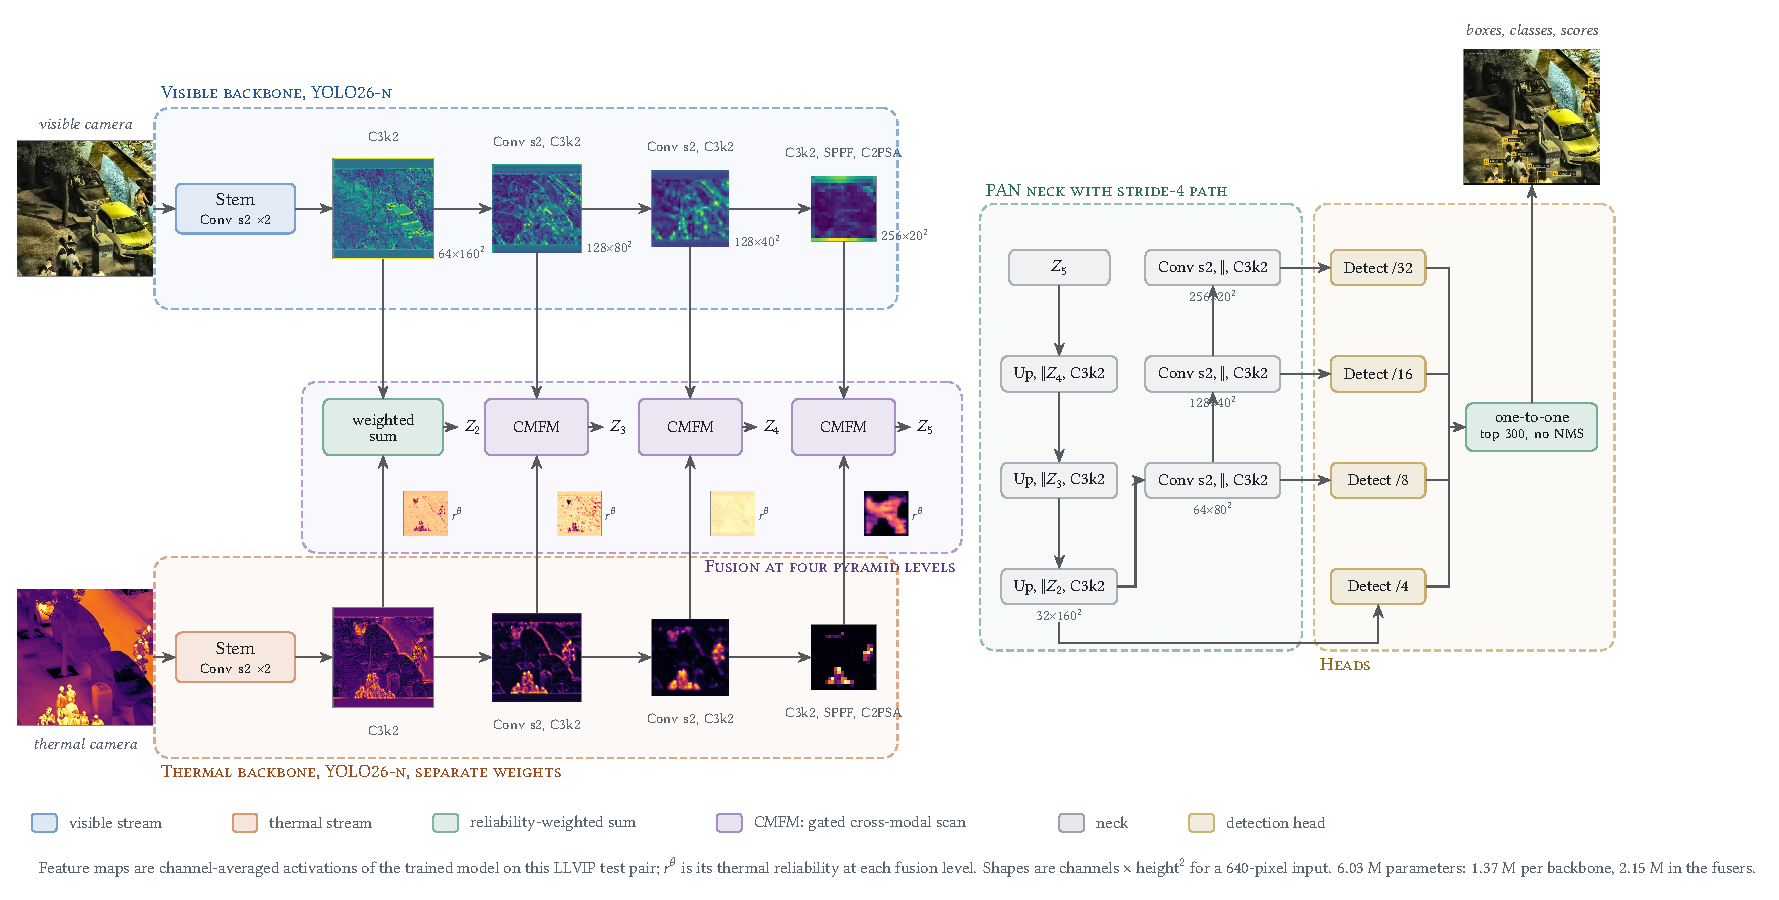
\includegraphics[width=0.92\textwidth]{figures/fig_cffm_overall.pdf}
\caption{CFFM-Net v1 on a LLVIP pair. Two YOLO26-n backbones with separate weights are fused at each pyramid level; the neck and head are stock YOLO26. The thermal reliability $\rt$ is shown at each level. Versions v2 and v3 drop the stride-4 level and its detection head.}
\label{fig:overall}
\end{figure*}

At night a visible camera sees little and a thermal camera sees warm bodies without texture, so pairing the two is the standard answer for pedestrian and vehicle detection after dark. The pairing carries a cost that benchmark tables hide. Public paired datasets are curated so that both streams are present, registered and healthy in every frame. A deployed pair is none of those things for long: the visible camera is blinded by headlights, the thermal core stalls during a shutter calibration, a lens knock shifts one image against the other, and a cable pull removes a stream entirely. A fusion network trained only on clean pairs has never been asked what to do when one input is wrong, and a detector that falls below its single-camera baseline in that moment is a worse sensor than either camera alone.

Recent fusion detectors build on selective state-space models~\cite{gu2023mamba}. Fusion-Mamba and CFMW scan the two modalities jointly and weight them afterwards~\cite{dong2025fusionmamba,li2025cfmw}, and transformer fusers such as CFT and ICAFusion attend across modalities~\cite{fang2021cft,shen2024icafusion}. As far as their descriptions show, in each case the combination rule acts on features that a faulty camera has already shaped. In a selective scan the shaping happens early, because every token writes into a recurrent state through its own step size, and a corrupted token writes just as strongly as a clean one.

CFFM-Net (Cross-Feature Fusion Mamba Network) moves the decision to where the write happens. A small head predicts a reliability in $(0,1)$ for each camera at each location, and the scan multiplies the step size of a token by the reliability of the camera it came from. The fusion block sits on top of a stock YOLO26 detector~\cite{yolo26_2026}, so the trainer, loss and evaluation are unchanged.

The evidence is mixed in places, and we report it that way. Over \resLlvipCffmVtwoSeedCount{} seeds the model beats a matched concatenation baseline on M3FD by \marMfdVtwoVsConcatMdMeanMap{}\,$\pm$\,\marMfdVtwoVsConcatMdStdMap{} mAP, which is not significant at $n=3$ (paired $p=\sigMfdP{}$), and is level with it on LLVIP and on KAIST still images. Fusing the two cameras beats the best single camera on M3FD by \gainMfdCffmVtwoOverBestMeanMap{}\,mAP, but the concatenation baseline captures \gainMfdConcatMdOverBestMeanMap{}\,of it. On the fault benchmark a baseline trained with fault augmentation is more robust than our model, which limits what the reliability gate can claim. Our contributions are:
\begin{itemize}
\item a cross-modal fusion block, CMFM, that gates the discretisation step of a four-direction selective scan by per-pixel, per-camera reliability, as a drop-in extension of YOLO26 (Section~\ref{sec:method});
\item a controlled evaluation on LLVIP and M3FD with a matched baseline, three seeds, matched single-camera baselines, and an eleven-fault sensor benchmark with a fault-trained baseline, set beside published results with their protocol differences stated (Section~\ref{sec:experiments});
\item a Temporal State Memory that carries a per-pixel scan state across video frames, evaluated on KAIST, where it helps under thermal noise and visible darkness and not under thermal loss or in tracking (Section~\ref{sec:video}).
\end{itemize}
A live runtime with a stream health monitor, a multi-camera analytics layer and per-seed tables are described in the supplementary material.

\section{Related Work}
\label{sec:related}
\paragraph{Detectors and state-space models.}
Real-time detection rests on feature pyramids~\cite{lin2017fpn} and path aggregation~\cite{liu2018panet}, as in YOLO26~\cite{yolo26_2026}. Small objects remain the acknowledged failure case~\cite{wang2025hpsdetr,li2025cfmw}, so we report average precision by size band. Mamba makes the state-space step input dependent~\cite{gu2023mamba}; vision variants differ in how they order two-dimensional tokens~\cite{zhu2024vim,liu2024vmamba,hatamizadeh2025mambavision}, and Mamba YOLO and UAVDet bring it into YOLO-style detectors~\cite{wang2025mambayolo,yang2026uavdet}. Ours uses the four-direction order of VMamba with a small state (size \cfgDState{}).

\paragraph{Visible-thermal detection.}
Work on KAIST~\cite{hwang2015kaist} compared where the two streams should meet~\cite{liu2016halfway}, handled misalignment~\cite{zhang2019arcnn} and built interaction and guidance modules~\cite{zhang2019cian,zhang2021gaff,cao2023csaa}. Recent detectors are transformer fusers~\cite{fang2021cft,shen2024icafusion,shen2025irdfusion}, detection transformers with two inputs~\cite{xing2024msdetr,guo2024damsdet,xiao2024gmdetr}, or designs that change the pipeline around the detector~\cite{wan2025yolov11rgbt,zhang2024tfdet,zhang2024e2emfd,zhao2026rsdet}. State-space fusion has appeared in Fusion-Mamba~\cite{dong2025fusionmamba}, CFMW~\cite{li2025cfmw}, WaveMamba~\cite{zhu2025wavemamba} and DMM~\cite{zhou2024dmm}; as far as their titles and abstracts show, these use the scan to mix the modalities, and we found none that gates its step by a per-camera reliability. MambaST fuses a few consecutive frames~\cite{mambast2024}; our memory carries a state indefinitely, with decay tied to reliability and elapsed time.

\paragraph{Reliability and data.}
MBNet weights the streams by illumination~\cite{zhou2020mbnet}, MS-DETR adds a modality-balanced optimisation~\cite{xing2024msdetr}, and probabilistic ensembling fuses per-modality detections~\cite{chen2022proben}. In the works we surveyed, reliability weights the features or the fused output; we found no method that controls the step of the scan itself, and no benchmark that corrupts one camera with a range of physical faults, so Section~\ref{sec:experiments} builds one. We use LLVIP~\cite{jia2021llvip}, M3FD~\cite{liu2022tardal}, KAIST~\cite{hwang2015kaist,li2018kaistsanitized} and ByteTrack~\cite{zhang2022bytetrack}.

\section{Method}
\label{sec:method}
\paragraph{Detector and reliability head.}
CFFM-Net extends YOLO26-n. A pair enters as a four-channel tensor, visible BGR and one thermal grey channel repeated to three for its backbone. Two backbones with separate weights, both initialised from COCO-pretrained YOLO26-n, produce feature maps at each pyramid level. A fuser at each level combines the visible map $\Fv$ and the thermal map $\Ft$ into one map $Z$ of the same shape, and the stock YOLO26 neck and head consume the fused maps (Fig.~\ref{fig:overall}). The model subclasses the Ultralytics detector and keeps the loss and validator unchanged. For each level a head predicts how far each camera can be trusted at each cell, $\rv,\rt\in(0,1)^{h\times w}$:
\begin{equation}
[\rv,\rt]=\sigma\!\Big(W_r\,\phi\big([\Fv,\;\Ft,\;|\Fv-\Ft|]\big)\Big),
\end{equation}
where $\phi$ is a depthwise $3{\times}3$ convolution with batch normalisation and SiLU and $W_r$ a $1{\times}1$ convolution to two channels. $W_r$ starts at zero weight with a bias of \cfgInitBias{}, so both cameras are trusted at initialisation. An optional sensor flag $f\in\{0,1\}^2$ multiplies the output, so an external monitor can declare a camera dead. Before the scan, a small head predicts a displacement $\Delta=\delta_{\max}\tanh(g([\Fv,\Ft]))$ with $\delta_{\max}=\cfgMaxDisp{}$ cells and bilinear sampling resamples the thermal map, giving $\tilde F^{\theta}$; it starts as the identity warp.

\paragraph{Reliability-gated cross scan.}
Both maps are projected to $d=\max(16,\mathrm{round}(\cfgRatio{}\,c))$ channels by a $1{\times}1$ and a depthwise $3{\times}3$ convolution, giving $p^{v}$ and $p^{\theta}$. At every cell the visible and thermal tokens are placed next to each other, so a sequence of $L=2hw$ tokens alternates $p^{v}_1,p^{\theta}_1,p^{v}_2,p^{\theta}_2,\dots$ over the raster order. The block scans it in $K=\cfgDirections{}$ orders (rows and columns, forward and backward). For one direction, token $u_\ell$ with modality $m(\ell)\in\{v,\theta\}$ and grid position $\mathrm{pos}(\ell)$, the recurrence is
\begin{align}
\Delta_\ell &= \softplus\!\big(W_\Delta u_\ell + b_\Delta\big)\,\cdot\, r^{m(\ell)}_{\mathrm{pos}(\ell)},\\
h_\ell &= e^{\Delta_\ell A}\, h_{\ell-1} + \Delta_\ell\, B_\ell\, u_\ell,\\
y_\ell &= C_\ell\, h_\ell + D\, u_\ell,
\end{align}
with $A$ diagonal and negative (state size \cfgDState{}), and $B_\ell$, $C_\ell$ and the pre-activation of $\Delta_\ell$ produced from the token as in Mamba~\cite{gu2023mamba}. The only change from a standard selective scan is the last factor in the first line. When the reliability is zero, $\Delta_\ell=0$, the decay factor is one, the input term vanishes, and the state passes the token untouched, so a camera with zero reliability cannot alter what the scan carries forward. The four outputs are mapped back to the grid and summed.

\paragraph{CMFM and fusion levels.}
The Cross-Modal Fusion Mamba block (CMFM, Fig.~\ref{fig:cmfm}) concatenates the scanned outputs of both modalities and normalises them with a channel LayerNorm. A local branch applies a depthwise $3{\times}3$ convolution to the concatenation of $p^{v}$ and $p^{\theta}$ to restore the two-dimensional neighbourhood. A $1{\times}1$ convolution on both paths gives a residual $M$, and the block outputs
\begin{equation}
Z=\frac{\rv\,\Fv+\rt\,\tilde F^{\theta}}{\max(\rv+\rt,\,\cfgWeightFloor{})}+M.
\end{equation}
The projection producing $M$ starts at zero, so a fresh block is exactly a reliability-weighted average and the scan has to earn any change. The scan runs in single precision, with a fused CUDA kernel, a Triton kernel or a chunked PyTorch reference. The first version (v1) fuses four levels, with a reliability-weighted average at stride 4 and CMFM at strides 8, 16 and 32; versions v2 and v3 read the head at strides 8, 16 and 32 only. The baseline replaces every fuser by concatenation and a $1{\times}1$ convolution, the usual two-stream design.

\begin{figure}[t]
\centering
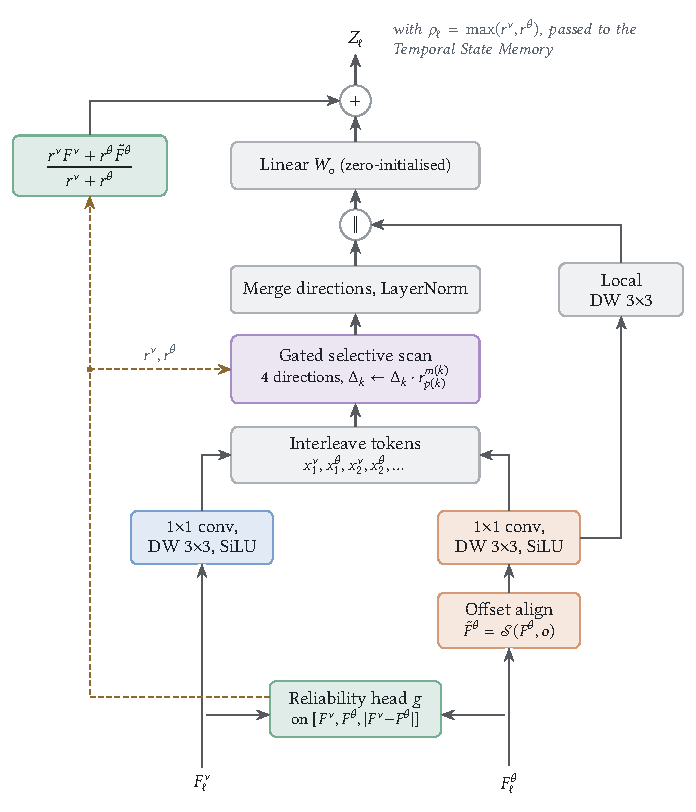
\includegraphics[width=0.78\columnwidth]{figures/fig_cmfm.pdf}
\caption{The CMFM block. A reliability head weights each camera, thermal features are warped onto the visible grid, visible and thermal tokens are interleaved and scanned in four directions with the step scaled by reliability, and a local convolution branch joins before a zero-initialised projection. The result adds to a reliability-weighted average.}
\label{fig:cmfm}
\end{figure}

\paragraph{Training recipes.}
\label{sec:recipes}
\emph{v1} uses four fusion levels and clean pairs. \emph{v2} uses three levels and \emph{modality dropout}: each training pair has probability \cfgMdProb{} of having its visible camera blacked out, and the same for the thermal camera; the control baseline is trained identically, so the comparison isolates the fuser. \emph{v3} adds \emph{fault training}, where with probability \cfgFaultProb{} one random camera is corrupted by a benchmark fault at random severity, and a \emph{reliability loss}, the binary cross-entropy between the mean reliability of each gated fuser and a trust target of \cfgTrustOne{}, \cfgTrustTwo{} or \cfgTrustThree{} at severity one, two or three (zero for a blacked-out camera, one for a healthy one), with weight \cfgRelWeight{}. The \emph{fault-trained concat} baseline keeps the fault training and the concat fuser.

\paragraph{Temporal State Memory.}
\label{sec:tsm}
A still-image detector forgets a pedestrian the moment its thermal camera drops a frame. The Temporal State Memory (TSM) gives each fusion level a per-pixel recurrent state across frames, attached after the fuser with a residual path that starts at zero, so a fresh memory gives exactly the detections of the model without it. At frame $t$ the fused map is projected to $u_t=W_u Z_t$, every channel at every cell keeps a state of size \cfgMemState{}, and the update is a selective scan in time:
\begin{align}
\delta_t &= \softplus(W_\delta u_t)\cdot\frac{\tau_t}{\tau_0}\cdot\rho_t,\\
S_t &= e^{\delta_t A}\odot \mathcal{W}_{H_t}(S_{t-1}) + \delta_t\, B_t\, u_t,\\
y_t &= C_t\, S_t + D\, u_t,\qquad Z'_t = Z_t + W_o\,\mathrm{DW}(y_t).
\end{align}
Three factors act on the step. The ratio $\tau_t/\tau_0$ of the real gap since the previous frame to a nominal gap $\tau_0=\cfgTauZero{}$\,s makes the decay depend on elapsed time. The reliability $\rho_t=\max(\rv_t,\rt_t)$ from CMFM is high when at least one camera is trusted, so a frame in which neither is reliable writes little into the state. The warp $\mathcal{W}_{H_t}$ resamples the previous state under the frame-to-frame homography, so the memory follows a moving camera. The memory is trained with the detector frozen on clips of \cfgClipLen{} frames at stride \cfgClipStride{} from KAIST training sequences~\cite{hwang2015kaist}; with probability one half a clip receives a fault (drop, darkness, noise, glare or shift) from a random frame to its end. Video inference is causal, and detections feed ByteTrack~\cite{zhang2022bytetrack}.

\section{Experiments}
\label{sec:experiments}
\subsection{Setup}
\label{sec:setup}
LLVIP~\cite{jia2021llvip} is a registered visible-infrared set of night pedestrians; we train on every \cfgLlvipStride{}rd frame of the training split and evaluate on the full test split. M3FD~\cite{liu2022tardal} has multiple scenarios and classes and no official detection split, so we hold out a fixed random \cfgMfdValPercent{}\,\% of the pairs with a seeded split shared by every run. Images are resized to \cfgImgsz{} pixels. The baseline is the two-stream concatenation detector with the same backbones, neck and head and matched training. Every fusion run uses COCO-pretrained YOLO26-n weights, batch size \cfgBatch{} and the stock Ultralytics trainer. Round one (v1) trains \cfgEpochsPilot{} epochs on clean pairs at seed zero; later rounds train \cfgEpochs{} epochs with mosaic off for the last \cfgCloseMosaic{}. The headline comparison, v2 against the concat baseline with modality dropout, uses \cfgSeedCount{} seeds on both datasets; v3 and its controls use seed zero. The single-camera baselines are YOLO26-n on one stream, one seed; on M3FD they use the same pretrained weights, epochs and mosaic schedule as fusion with batch size 32, and on LLVIP they ran \cfgEpochsPilot{} epochs and are not matched. We report percent as mean $\pm$ sample standard deviation over seeds ($n=3$); margins are means of per-seed differences in percentage points (pp). We report COCO-style mAP at IoU 0.5 to 0.95 and at 0.5 (mAP$_{50}$) and average precision by size band. Latency is batch one at \cfgLatH{}$\times$\cfgLatW{} in half precision, after \cfgLatWarmup{} warm-up and over \cfgLatIters{} timed iterations.

\paragraph{Sensor-fault benchmark.}
Eleven physically motivated faults are applied to one camera of the test pairs at three severities: the visible camera suffers darkness, glare, fog, noise, blur and a full drop; the thermal camera suffers a full drop, a spatial shift, column banding with pixel noise, loss of contrast toward the scene mean, and dead pixels. We tabulate severity three. In two further rows the dropped camera is declared by the sensor flag. v2 and the concat baseline are scored with the checkpoints of all three seeds on M3FD and with the seed-zero checkpoints on LLVIP; the fault-trained concat baseline is scored at seed zero.

\subsection{Main results}
\label{sec:main}
\begin{table}[t]
\centering
\caption{Detection accuracy in percent. Fusion models: mean and sample std over three seeds, 80 epochs. Single-camera rows: one seed; 30 epochs on LLVIP, which is not matched to the fusion rows, and 80 epochs on M3FD, which is. The margin over the best single camera subtracts the one-seed single-camera value from each fusion seed.}
\label{tab:main}
{\footnotesize\setlength{\tabcolsep}{4pt}
\adjustbox{max width=\linewidth}{\begin{tabular}{lcc}
\toprule
Model & mAP & mAP$_{50}$ \\
\midrule
\multicolumn{3}{l}{\emph{LLVIP}} \\
YOLO26-n visible & \resLlvipYoloVisSeedZeroMap & \resLlvipYoloVisSeedZeroMapFifty \\
YOLO26-n thermal & \resLlvipYoloThmSeedZeroMap & \resLlvipYoloThmSeedZeroMapFifty \\
Concat, modality dropout & \resLlvipConcatMdMeanMap\,\ensuremath{\pm}\,\resLlvipConcatMdStdMap & \resLlvipConcatMdMeanMapFifty\,\ensuremath{\pm}\,\resLlvipConcatMdStdMapFifty \\
CFFM-Net v2 & \resLlvipCffmVtwoMeanMap\,\ensuremath{\pm}\,\resLlvipCffmVtwoStdMap & \resLlvipCffmVtwoMeanMapFifty\,\ensuremath{\pm}\,\resLlvipCffmVtwoStdMapFifty \\
Margin of v2 over concat (pp) & \marLlvipVtwoVsConcatMdMeanMap\,\ensuremath{\pm}\,\marLlvipVtwoVsConcatMdStdMap & \marLlvipVtwoVsConcatMdMeanMapFifty\,\ensuremath{\pm}\,\marLlvipVtwoVsConcatMdStdMapFifty \\
\midrule
\multicolumn{3}{l}{\emph{M3FD}} \\
YOLO26-n visible & \resMfdYoloVisSeedZeroMap & \resMfdYoloVisSeedZeroMapFifty \\
YOLO26-n thermal & \resMfdYoloThmSeedZeroMap & \resMfdYoloThmSeedZeroMapFifty \\
Concat, modality dropout & \resMfdConcatMdMeanMap\,\ensuremath{\pm}\,\resMfdConcatMdStdMap & \resMfdConcatMdMeanMapFifty\,\ensuremath{\pm}\,\resMfdConcatMdStdMapFifty \\
CFFM-Net v2 & \resMfdCffmVtwoMeanMap\,\ensuremath{\pm}\,\resMfdCffmVtwoStdMap & \resMfdCffmVtwoMeanMapFifty\,\ensuremath{\pm}\,\resMfdCffmVtwoStdMapFifty \\
Margin of v2 over concat (pp) & \marMfdVtwoVsConcatMdMeanMap\,\ensuremath{\pm}\,\marMfdVtwoVsConcatMdStdMap & \marMfdVtwoVsConcatMdMeanMapFifty\,\ensuremath{\pm}\,\marMfdVtwoVsConcatMdStdMapFifty \\
Margin of v2 over best single camera (pp) & \gainMfdCffmVtwoOverBestMeanMap\,\ensuremath{\pm}\,\gainMfdCffmVtwoOverBestStdMap & \gainMfdCffmVtwoOverBestMapFiftyMean\,\ensuremath{\pm}\,\gainMfdCffmVtwoOverBestMapFiftyStd \\
\bottomrule
\end{tabular}}}
\end{table}

Table~\ref{tab:main} gives the headline comparison. On M3FD, CFFM-Net v2 reaches \resMfdCffmVtwoMeanMap{}\,$\pm$\,\resMfdCffmVtwoStdMap{} mAP against \resMfdConcatMdMeanMap{}\,$\pm$\,\resMfdConcatMdStdMap{} for the concat baseline, a margin of \marMfdVtwoVsConcatMdMeanMap{}\,$\pm$\,\marMfdVtwoVsConcatMdStdMap{}\,pp, ahead on every one of the three seeds. The margin is small and not significant at $n=3$: the paired $t$-test gives $p=\sigMfdP{}$ and the 95\,\% confidence interval is \sigMfdCiLow{} to \sigMfdCiHigh{}\,pp. On LLVIP the two models are level, with a margin of \marLlvipVtwoVsConcatMdMeanMap{}\,$\pm$\,\marLlvipVtwoVsConcatMdStdMap{}\,pp whose spread exceeds its mean (paired $p=\sigLlvipP{}$), and we read it as a tie. On small objects v2 gains \marMfdVtwoVsConcatMdMeanApSmall{}\,$\pm$\,\marMfdVtwoVsConcatMdStdApSmall{}\,pp on M3FD, the only size band whose spread is smaller than its mean and not significant at $n=3$, and \marLlvipVtwoVsConcatMdMeanApSmall{}\,pp on LLVIP, so we claim no small-object advantage; the supplement lists every band.

The single-camera rows give context. On M3FD the matched baselines reach \resMfdYoloVisSeedZeroMap{} mAP on the visible images and \resMfdYoloThmSeedZeroMap{} on the thermal images, so the visible camera is the stronger one. CFFM-Net v2 is \gainMfdCffmVtwoOverBestMeanMap{}\,$\pm$\,\gainMfdCffmVtwoOverBestStdMap{}\,pp above it (\gainMfdCffmVtwoOverBestMinMap{}\,pp on its lowest seed), and the concat baseline is \gainMfdConcatMdOverBestMeanMap{}\,$\pm$\,\gainMfdConcatMdOverBestStdMap{}\,pp above it. Most of the gain from fusing the two cameras is therefore available to the plain baseline. The single-camera values are one seed and use twice the fusion batch size, so the true uncertainty of the gain is larger. On LLVIP the single-camera rows are not matched (\resLlvipYoloVisSeedZeroMap{} and \resLlvipYoloThmSeedZeroMap{} mAP at \cfgEpochsPilot{} epochs against \cfgEpochs{}) and support no conclusion about the gain from fusion there.

\subsection{Sensor faults}
\label{sec:faults}
\begin{table*}[t]
\centering
\caption{Fault benchmark at severity three, mAP in percent, 80 epochs. LLVIP is seed 0 only. On M3FD the v2 and concat columns (modality dropout) are mean and sample std over three seeds, and the fault-trained concat column (Concat FT) is seed 0. Flagged rows tell the model which camera dropped.}
\label{tab:fault}
{\footnotesize\setlength{\tabcolsep}{4pt}
\adjustbox{max width=\linewidth}{\begin{tabular}{lcccccc}
\toprule
& \multicolumn{3}{c}{LLVIP, seed 0} & \multicolumn{3}{c}{M3FD, mean \ensuremath{\pm} std, three seeds} \\ \cmidrule(lr){2-4}\cmidrule(lr){5-7} Fault & v2 & Concat & Concat FT & v2 & Concat & Concat FT \\
\midrule
Clean & \fltLlvipCffmVtwoCleanMap & \fltLlvipConcatMdCleanMap & \fltLlvipConcatFtCleanMap & \fltMfdCffmVtwoCleanMeanMap\,\ensuremath{\pm}\,\fltMfdCffmVtwoCleanStdMap & \fltMfdConcatMdCleanMeanMap\,\ensuremath{\pm}\,\fltMfdConcatMdCleanStdMap & \fltMfdConcatFtCleanMap \\
\midrule
Visible dark & \fltLlvipCffmVtwoVisibleDarkThreeMap & \fltLlvipConcatMdVisibleDarkThreeMap & \fltLlvipConcatFtVisibleDarkThreeMap & \fltMfdCffmVtwoVisibleDarkThreeMeanMap\,\ensuremath{\pm}\,\fltMfdCffmVtwoVisibleDarkThreeStdMap & \fltMfdConcatMdVisibleDarkThreeMeanMap\,\ensuremath{\pm}\,\fltMfdConcatMdVisibleDarkThreeStdMap & \fltMfdConcatFtVisibleDarkThreeMap \\
Visible glare & \fltLlvipCffmVtwoVisibleGlareThreeMap & \fltLlvipConcatMdVisibleGlareThreeMap & \fltLlvipConcatFtVisibleGlareThreeMap & \fltMfdCffmVtwoVisibleGlareThreeMeanMap\,\ensuremath{\pm}\,\fltMfdCffmVtwoVisibleGlareThreeStdMap & \fltMfdConcatMdVisibleGlareThreeMeanMap\,\ensuremath{\pm}\,\fltMfdConcatMdVisibleGlareThreeStdMap & \fltMfdConcatFtVisibleGlareThreeMap \\
Visible fog & \fltLlvipCffmVtwoVisibleFogThreeMap & \fltLlvipConcatMdVisibleFogThreeMap & \fltLlvipConcatFtVisibleFogThreeMap & \fltMfdCffmVtwoVisibleFogThreeMeanMap\,\ensuremath{\pm}\,\fltMfdCffmVtwoVisibleFogThreeStdMap & \fltMfdConcatMdVisibleFogThreeMeanMap\,\ensuremath{\pm}\,\fltMfdConcatMdVisibleFogThreeStdMap & \fltMfdConcatFtVisibleFogThreeMap \\
Visible noise & \fltLlvipCffmVtwoVisibleNoiseThreeMap & \fltLlvipConcatMdVisibleNoiseThreeMap & \fltLlvipConcatFtVisibleNoiseThreeMap & \fltMfdCffmVtwoVisibleNoiseThreeMeanMap\,\ensuremath{\pm}\,\fltMfdCffmVtwoVisibleNoiseThreeStdMap & \fltMfdConcatMdVisibleNoiseThreeMeanMap\,\ensuremath{\pm}\,\fltMfdConcatMdVisibleNoiseThreeStdMap & \fltMfdConcatFtVisibleNoiseThreeMap \\
Visible blur & \fltLlvipCffmVtwoVisibleBlurThreeMap & \fltLlvipConcatMdVisibleBlurThreeMap & \fltLlvipConcatFtVisibleBlurThreeMap & \fltMfdCffmVtwoVisibleBlurThreeMeanMap\,\ensuremath{\pm}\,\fltMfdCffmVtwoVisibleBlurThreeStdMap & \fltMfdConcatMdVisibleBlurThreeMeanMap\,\ensuremath{\pm}\,\fltMfdConcatMdVisibleBlurThreeStdMap & \fltMfdConcatFtVisibleBlurThreeMap \\
Visible drop & \fltLlvipCffmVtwoVisibleDropThreeMap & \fltLlvipConcatMdVisibleDropThreeMap & \fltLlvipConcatFtVisibleDropThreeMap & \fltMfdCffmVtwoVisibleDropThreeMeanMap\,\ensuremath{\pm}\,\fltMfdCffmVtwoVisibleDropThreeStdMap & \fltMfdConcatMdVisibleDropThreeMeanMap\,\ensuremath{\pm}\,\fltMfdConcatMdVisibleDropThreeStdMap & \fltMfdConcatFtVisibleDropThreeMap \\
Thermal drop & \fltLlvipCffmVtwoThermalDropThreeMap & \fltLlvipConcatMdThermalDropThreeMap & \fltLlvipConcatFtThermalDropThreeMap & \fltMfdCffmVtwoThermalDropThreeMeanMap\,\ensuremath{\pm}\,\fltMfdCffmVtwoThermalDropThreeStdMap & \fltMfdConcatMdThermalDropThreeMeanMap\,\ensuremath{\pm}\,\fltMfdConcatMdThermalDropThreeStdMap & \fltMfdConcatFtThermalDropThreeMap \\
Thermal shift & \fltLlvipCffmVtwoThermalShiftThreeMap & \fltLlvipConcatMdThermalShiftThreeMap & \fltLlvipConcatFtThermalShiftThreeMap & \fltMfdCffmVtwoThermalShiftThreeMeanMap\,\ensuremath{\pm}\,\fltMfdCffmVtwoThermalShiftThreeStdMap & \fltMfdConcatMdThermalShiftThreeMeanMap\,\ensuremath{\pm}\,\fltMfdConcatMdThermalShiftThreeStdMap & \fltMfdConcatFtThermalShiftThreeMap \\
Thermal noise & \fltLlvipCffmVtwoThermalNoiseThreeMap & \fltLlvipConcatMdThermalNoiseThreeMap & \fltLlvipConcatFtThermalNoiseThreeMap & \fltMfdCffmVtwoThermalNoiseThreeMeanMap\,\ensuremath{\pm}\,\fltMfdCffmVtwoThermalNoiseThreeStdMap & \fltMfdConcatMdThermalNoiseThreeMeanMap\,\ensuremath{\pm}\,\fltMfdConcatMdThermalNoiseThreeStdMap & \fltMfdConcatFtThermalNoiseThreeMap \\
Thermal crossover & \fltLlvipCffmVtwoThermalCrossoverThreeMap & \fltLlvipConcatMdThermalCrossoverThreeMap & \fltLlvipConcatFtThermalCrossoverThreeMap & \fltMfdCffmVtwoThermalCrossoverThreeMeanMap\,\ensuremath{\pm}\,\fltMfdCffmVtwoThermalCrossoverThreeStdMap & \fltMfdConcatMdThermalCrossoverThreeMeanMap\,\ensuremath{\pm}\,\fltMfdConcatMdThermalCrossoverThreeStdMap & \fltMfdConcatFtThermalCrossoverThreeMap \\
Thermal dead & \fltLlvipCffmVtwoThermalDeadThreeMap & \fltLlvipConcatMdThermalDeadThreeMap & \fltLlvipConcatFtThermalDeadThreeMap & \fltMfdCffmVtwoThermalDeadThreeMeanMap\,\ensuremath{\pm}\,\fltMfdCffmVtwoThermalDeadThreeStdMap & \fltMfdConcatMdThermalDeadThreeMeanMap\,\ensuremath{\pm}\,\fltMfdConcatMdThermalDeadThreeStdMap & \fltMfdConcatFtThermalDeadThreeMap \\
Visible drop, flagged & \fltLlvipCffmVtwoVisibleDropThreeFlaggedMap & \fltLlvipConcatMdVisibleDropThreeFlaggedMap & \fltLlvipConcatFtVisibleDropThreeFlaggedMap & \fltMfdCffmVtwoVisibleDropThreeFlaggedMeanMap\,\ensuremath{\pm}\,\fltMfdCffmVtwoVisibleDropThreeFlaggedStdMap & \fltMfdConcatMdVisibleDropThreeFlaggedMeanMap\,\ensuremath{\pm}\,\fltMfdConcatMdVisibleDropThreeFlaggedStdMap & \fltMfdConcatFtVisibleDropThreeFlaggedMap \\
Thermal drop, flagged & \fltLlvipCffmVtwoThermalDropThreeFlaggedMap & \fltLlvipConcatMdThermalDropThreeFlaggedMap & \fltLlvipConcatFtThermalDropThreeFlaggedMap & \fltMfdCffmVtwoThermalDropThreeFlaggedMeanMap\,\ensuremath{\pm}\,\fltMfdCffmVtwoThermalDropThreeFlaggedStdMap & \fltMfdConcatMdThermalDropThreeFlaggedMeanMap\,\ensuremath{\pm}\,\fltMfdConcatMdThermalDropThreeFlaggedStdMap & \fltMfdConcatFtThermalDropThreeFlaggedMap \\
\midrule
Mean over faults & \fltLlvipCffmVtwoAvgSevThreeMap & \fltLlvipConcatMdAvgSevThreeMap & \fltLlvipConcatFtAvgSevThreeMap & \fltMfdCffmVtwoMeanAvgSevThreeMap\,\ensuremath{\pm}\,\fltMfdCffmVtwoStdAvgSevThreeMap & \fltMfdConcatMdMeanAvgSevThreeMap\,\ensuremath{\pm}\,\fltMfdConcatMdStdAvgSevThreeMap & \fltMfdConcatFtAvgSevThreeMap \\
Retained (\%) & \fltLlvipCffmVtwoRetainedSevThreePercent & \fltLlvipConcatMdRetainedSevThreePercent & \fltLlvipConcatFtRetainedSevThreePercent & \fltMfdCffmVtwoMeanRetainedSevThreePercent\,\ensuremath{\pm}\,\fltMfdCffmVtwoStdRetainedSevThreePercent & \fltMfdConcatMdMeanRetainedSevThreePercent\,\ensuremath{\pm}\,\fltMfdConcatMdStdRetainedSevThreePercent & \fltMfdConcatFtRetainedSevThreePercent \\
\bottomrule
\end{tabular}}}
\end{table*}

Table~\ref{tab:fault} reports the benchmark. On M3FD every number for v2 and the modality-dropout baseline is a mean over three seeds; on LLVIP it is one seed, where seed-to-seed spread of clean mAP is about one point, so differences of one to three points are within noise. Averaged over the eleven faults, v2 keeps \fltMfdCffmVtwoMeanRetainedSevThreePercent{}\,$\pm$\,\fltMfdCffmVtwoStdRetainedSevThreePercent{}\,\% of its clean mAP on M3FD against \fltMfdConcatMdMeanRetainedSevThreePercent{}\,$\pm$\,\fltMfdConcatMdStdRetainedSevThreePercent{}\,\% for the concat baseline, and \fltLlvipCffmVtwoRetainedSevThreePercent{}\,\% against \fltLlvipConcatMdRetainedSevThreePercent{}\,\% on LLVIP. A thermal shift is the worst fault for every model.

The comparison depends on the camera that fails (the supplement plots the margins). On M3FD, v2 is ahead on every thermal-side fault (dead pixels by \fltMfdMarginThermalDeadSevThreeMeanMap{}\,pp, noise \fltMfdMarginThermalNoiseSevThreeMeanMap{}, shift \fltMfdMarginThermalShiftSevThreeMeanMap{}, crossover \fltMfdMarginThermalCrossoverSevThreeMeanMap{}, a thermal drop \fltMfdMarginThermalDropSevThreeMeanMap{}) and behind on every visible-side fault, from \fltMfdMarginVisibleDarkSevThreeMeanMap{} (darkness) to \fltMfdMarginVisibleNoiseSevThreeMeanMap{}\,pp (noise). Averaged over each camera's faults the margin is \fltMfdMarginMeanThermalAvgSevThreeMap{}\,$\pm$\,\fltMfdMarginStdThermalAvgSevThreeMap{}\,pp for thermal faults and \fltMfdMarginMeanVisibleAvgSevThreeMap{}\,$\pm$\,\fltMfdMarginStdVisibleAvgSevThreeMap{}\,pp for visible faults, and over all eleven \fltMfdMarginMeanAvgSevThreeMap{}\,$\pm$\,\fltMfdMarginStdAvgSevThreeMap{}\,pp (paired $p=\fltMfdMarginAvgP{}$, 95\,\% interval \fltMfdMarginAvgCiLow{} to \fltMfdMarginAvgCiHigh{}\,pp), not significant at $n=3$. The sign of the per-fault margin agrees on all three seeds for \fltMfdSignAgreeSevThree{} of the \fltMfdFaultCount{} faults, so we read the thermal-side advantage as a pattern the data support without a significance test passed. It is plausible for the design: when the thermal stream is degraded the gate can lower its weight and the scan writes less of it into the state, while visible-side faults are corrupted before the visible features exist. On LLVIP, with one seed, v2 is ahead on \fltLlvipWinsSevThree{} of the eleven faults, including darkness (\fltLlvipMarginVisibleDarkSevThreeMap{}\,pp), but loses heavily to additive noise on either camera (\fltLlvipMarginVisibleNoiseSevThreeMap{} and \fltLlvipMarginThermalNoiseSevThreeMap{}\,pp) and to dead thermal pixels (\fltLlvipMarginThermalDeadSevThreeMap{}); the mean margin is \fltLlvipMarginAvgSevThreeMap{}\,pp. The gate is not a general robustness mechanism.

The strongest result of the benchmark concerns neither fusion design. A concat baseline trained with fault augmentation (Concat FT, seed zero) retains \fltMfdConcatFtRetainedSevThreePercent{}\,\% of its clean mAP on M3FD and \fltLlvipConcatFtRetainedSevThreePercent{}\,\% on LLVIP, against \fltMfdCffmVtwoMeanRetainedSevThreePercent{}\,\% and \fltLlvipCffmVtwoRetainedSevThreePercent{}\,\% for v2. Its mean mAP over the faults is higher than that of v2 by \fltMfdVtwoVsConcatFtGapSevThreeMap{}\,pp on M3FD and \fltLlvipVtwoVsConcatFtGapSevThreeMap{}\,pp on LLVIP, while its clean mAP is within one point of v2 (\fltMfdVtwoVsConcatFtCleanMap{}\,pp and \fltLlvipVtwoVsConcatFtCleanMap{}\,pp). Training on faulty inputs buys more robustness than the reliability-gated scan, at no cost in clean accuracy. Telling the model which camera dropped through the sensor flag changes nothing measurable (flagged and unflagged rows differ by at most two tenths of a point).

\subsection{Ablations and the negative result}
\label{sec:ablation}
The supplement lists every variant. Round one was negative: CFFM-Net v1 had a margin of \marLlvipVoneVsConcatPlainSeedZeroMap{}\,pp on LLVIP and \marMfdVoneVsConcatPlainSeedZeroMap{}\,pp on M3FD against the concat baseline. Part of the gap came from the stride-4 level: adding that head lowers the concat baseline from \resLlvipConcatPlainSeedZeroMap{} to \resLlvipConcatPtwoSeedZeroMap{} on LLVIP, and against the concat baseline with the same head the margin of v1 is \marLlvipVoneVsConcatPtwoSeedZeroMap{}\,pp. We therefore dropped the stride-4 level in v2, a decision made on LLVIP at seed zero. Removing the gate costs v1 \marLlvipVoneVsVoneNogateSeedZeroMap{}\,pp and replacing the scan by a gated convolution of matched cost \marLlvipVoneVsVoneGconvSeedZeroMap{}\,pp, both within the noise of one seed, so we do not claim that the scan or the gate, on their own, explain the v2 gain; the v2 comparison is between complete systems. v3 failed in a preliminary single-seed result: \resLlvipCffmVthreeSeedZeroMap{} mAP on LLVIP and \resMfdCffmVthreeSeedZeroMap{} on M3FD, below v2 (\marLlvipVthreeVsVtwoSeedZeroMap{} and \marMfdVthreeVsVtwoSeedZeroMap{}\,pp) and below the fault-trained concat baseline, and \marLlvipVthreeVsVthreeNorelSeedZeroMap{} and \marMfdVthreeVsVthreeNorelSeedZeroMap{}\,pp against its no-reliability-branch control. We report the reliability loss as a negative ablation and leave it out of the recipe; the sign agrees on both datasets but the size of the effect is uncertain.

\subsection{Cost}
\label{sec:cost}
The supplement tabulates the cost of every model on a \latLocalDevice{}. CFFM-Net v2 has \latLocalVtwoParamsM{}\,M parameters and \latLocalVtwoGflops{} GFLOPs, a median latency of \latLocalVtwoMedianMs{}\,ms (about \latLocalVtwoFps{} frames per second) and a 95th percentile of \latLocalVtwoPNinetyFiveMs{}\,ms. Against the concat baseline this is \latLocalRatioParams{} times the parameters, \latLocalRatioGflops{} times the FLOPs and \latLocalRatioMedian{} times the median latency, so v2 passes the limit of at most twice the baseline latency that was fixed in advance.

\subsection{Context with published detectors}
\label{sec:sota}
Published numbers differ in backbone, input size, schedule, annotations and split, so the experiments above compare CFFM-Net with a matched baseline. Table~\ref{tab:sota} nevertheless places our results beside published figures, copied from the cited papers and not re-run; the supplement does the same for KAIST. Our models are nano scale (\latLocalVtwoParamsM{}\,M parameters, \latLocalVtwoGflops{} GFLOPs); we make no claim about relative efficiency.

\begin{table*}[t]
\centering
\caption{Published RGB-T detection results for context, in percent. Numbers are copied from the cited papers, not re-run. Input size or split is stated per row because mAP depends on both. Our models are nano scale, trained on one third of the LLVIP training frames (mean of three seeds), so they are not a like-for-like comparison. On M3FD no row shares a split with ours, and no ranking is claimed.}
\label{tab:sota}
{\footnotesize\setlength{\tabcolsep}{4pt}
\adjustbox{max width=\linewidth}{\begin{tabular}{lllcc}
\toprule
Method & Detector & Input or split & mAP$_{50}$ & mAP \\
\midrule
\multicolumn{5}{l}{\emph{LLVIP, official split (12,025 / 3,463 pairs)}} \\
YOLOv5-l, infrared only~\cite{jia2021llvip} & YOLOv5-l & not stated & 96.5 & 67.0 \\
CFT~\cite{fang2021cft} & YOLOv5 with CFB & 640$\times$640 & 97.5 & 63.6 \\
CSSA~\cite{cao2023csaa} & Faster R-CNN, ResNet-50 & 640$\times$512 & 94.3 & 59.2 \\
MS-DETR~\cite{xing2024msdetr} & Deformable DETR, ResNet-50 & 640$\times$512 & 97.9 & 66.1 \\
Fusion-Mamba~\cite{dong2025fusionmamba} & YOLOv8-l & 640$\times$640 & 97.0 & 64.3 \\
DAMSDet~\cite{guo2024damsdet} & DETR, ResNet-50 & 1024$\times$1024 & 97.9 & 69.6 \\
TFDet~\cite{zhang2024tfdet} & YOLOv5-l & not stated & 97.9 & 71.1 \\
WaveMamba~\cite{zhu2025wavemamba} & YOLOv8 & not stated & 98.3 & 66.0 \\
IRDFusion~\cite{shen2025irdfusion} & Co-DETR & 640$\times$640 & 98.4 & 70.9 \\
CFFM-Net v2 (this work) & YOLO26-n, \latLocalVtwoParamsM{}\,M & \cfgImgsz{}, every third frame & \resLlvipCffmVtwoMeanMapFifty & \resLlvipCffmVtwoMeanMap \\
Concat baseline (this work) & YOLO26-n, \latLocalConcatMdParamsM{}\,M & \cfgImgsz{}, every third frame & \resLlvipConcatMdMeanMapFifty & \resLlvipConcatMdMeanMap \\
\midrule
\multicolumn{5}{l}{\emph{M3FD, splits differ between rows and are not comparable}} \\
TarDAL, fused image~\cite{liu2022tardal} & YOLOv5 & 3,500 train, test not stated & 80.7 & -- \\
DAMSDet~\cite{guo2024damsdet} & DETR, ResNet-50 & 3,368 / 831, by scene & 80.2 & 52.9 \\
TFDet~\cite{zhang2024tfdet} & YOLOv5 & 2,905 / 1,295 & 64.8 & 41.0 \\
E2E-MFD~\cite{zhang2024e2emfd} & Detectron2, end to end & 2,940 / 1,260 & 91.8 & 63.8 \\
Fusion-Mamba~\cite{dong2025fusionmamba} & YOLOv8-l & split of Liang et al. & 88.0 & 61.9 \\
WaveMamba~\cite{zhu2025wavemamba} & YOLOv8 & 3,360 / 840 & 92.1 & 64.4 \\
CFFM-Net v2 (this work) & YOLO26-n, \latLocalVtwoParamsM{}\,M & 3,360 / 840, random & \resMfdCffmVtwoMeanMapFifty & \resMfdCffmVtwoMeanMap \\
Concat baseline (this work) & YOLO26-n, \latLocalConcatMdParamsM{}\,M & 3,360 / 840, random & \resMfdConcatMdMeanMapFifty & \resMfdConcatMdMeanMap \\
\bottomrule
\end{tabular}}}
\end{table*}


On LLVIP, with the official split, v2 reaches \resLlvipCffmVtwoMeanMapFifty{}\,\% mAP$_{50}$ and \resLlvipCffmVtwoMeanMap{}\,\% mAP, in the range of published fusion results (mAP from \sotaLlvipFusionMapMin{} to \sotaLlvipFusionMapMax{}) and below the best of them, with training on one third of the frames and no large backbone. The comparison is weaker than it looks: the infrared-only YOLOv5-l baseline already reaches \sotaLlvipIrOnlyMap{} mAP in the dataset paper~\cite{jia2021llvip}, so thermal imagery nearly saturates the benchmark. On M3FD no row shares our split, published mAP$_{50}$ runs from \sotaMfdMapFiftyMin{} to \sotaMfdMapFiftyMax{}, and CFT is reported \sotaMfdSplitSwing{} points apart in two cited papers with different splits, so we draw no ranking. On KAIST our miss rates (\kstConcatAllMr{}\,\% for the concat baseline, \kstCffmAllMr{}\,\% for v2) are far above the published \sotaKaistMrMin{} to \sotaKaistMrMax{}, obtained with ResNet or VGG backbones, sanitised training annotations and the standard evaluation code. We attribute part of the gap to protocol and part to scale and a short schedule but did not apportion it; our KAIST detectors are not competitive with the published state of the art.

\section{Video Experiments on KAIST}
\label{sec:video}
\subsection{Protocol}
\label{sec:kaistprotocol}
\begin{table*}[t]
\centering
\caption{Temporal State Memory against the same detector without memory on KAIST. A camera fails for four seconds in every eight. Failed frames are those inside a failure. Change is memory minus image. One memory training run, one detector.}
\label{tab:memory}
{\footnotesize\setlength{\tabcolsep}{4pt}
\adjustbox{max width=\linewidth}{\begin{tabular}{lcccccc}
\toprule
& \multicolumn{3}{c}{All frames} & \multicolumn{3}{c}{Failed frames} \\ \cmidrule(lr){2-4}\cmidrule(lr){5-7} Condition & Image & Memory & Change & Image & Memory & Change \\
\midrule
\multicolumn{7}{l}{\emph{Miss rate (\%), lower is better}} \\
Clean & \memCleanImageAllMr & \memCleanMemoryAllMr & \memChangeCleanAllMr & -- & -- & -- \\
Thermal lost & \memThermalLostImageAllMr & \memThermalLostMemoryAllMr & \memChangeThermalLostAllMr & \memThermalLostImageFailedMr & \memThermalLostMemoryFailedMr & \memChangeThermalLostFailedMr \\
Thermal lost, flagged & \memThermalLostFlaggedImageAllMr & \memThermalLostFlaggedMemoryAllMr & \memChangeThermalLostFlaggedAllMr & \memThermalLostFlaggedImageFailedMr & \memThermalLostFlaggedMemoryFailedMr & \memChangeThermalLostFlaggedFailedMr \\
Visible dark & \memVisibleDarkImageAllMr & \memVisibleDarkMemoryAllMr & \memChangeVisibleDarkAllMr & \memVisibleDarkImageFailedMr & \memVisibleDarkMemoryFailedMr & \memChangeVisibleDarkFailedMr \\
Thermal noise & \memThermalNoiseImageAllMr & \memThermalNoiseMemoryAllMr & \memChangeThermalNoiseAllMr & \memThermalNoiseImageFailedMr & \memThermalNoiseMemoryFailedMr & \memChangeThermalNoiseFailedMr \\
\midrule
\multicolumn{7}{l}{\emph{Tracking, mean of four sequences}} \\ & \multicolumn{3}{c}{MOTA (\%)} & \multicolumn{3}{c}{IDF1 (\%)} \\ \cmidrule(lr){2-4}\cmidrule(lr){5-7} Condition & Image & Memory & Change & Image & Memory & Change \\
Clean & \trkCleanImageMota & \trkCleanMemoryMota & \trkChangeCleanMota & \trkCleanImageIdfOne & \trkCleanMemoryIdfOne & \trkChangeCleanIdfOne \\
Thermal lost & \trkThermalLostImageMota & \trkThermalLostMemoryMota & \trkChangeThermalLostMota & \trkThermalLostImageIdfOne & \trkThermalLostMemoryIdfOne & \trkChangeThermalLostIdfOne \\
\bottomrule
\end{tabular}}}
\end{table*}


KAIST~\cite{hwang2015kaist} supplies visible and thermal video at 20 frames per second. We use the standard split (sets 00 to 05 for training, 06 to 11 for testing; sets 00 to 02 and 06 to 08 by day, the rest at night). The still-image detectors, CFFM-Net v2 and the concat baseline with modality dropout, train on every \cfgKaistTrainStride{}th frame of the training sets, with persons at least \cfgKaistTrainMinH{} pixels tall as targets, for \cfgKaistEpochs{} epochs at seed zero. The test frames are every \cfgKaistTestStride{}th frame, \kstNAll{} of which \kstNDay{} are by day and \kstNNight{} by night. The metric is the log-average miss rate (MR) over nine false-positives-per-image values between $10^{-2}$ and $10^{0}$ on the reasonable subset (persons at least \cfgKaistMinH{} pixels tall, visible fraction at least \cfgKaistMinVis{}); lower is better. We use the original annotations and our own implementation of the Caltech matching protocol, and not the sanitised annotations~\cite{li2018kaistsanitized}, so the miss rates are internally consistent but not comparable with published figures. For video the detector runs causally at \cfgFailFps{} frames per second. A failure schedule repeats \cfgFailSeconds{} healthy and \cfgFailSeconds{} failed seconds, with conditions a lost thermal camera (a black image), the same declared by the sensor flag, a darkened visible camera and additive thermal noise, all at severity three. Detector weights are identical in every row; only the memory is switched on or off at test time. Tracking uses ByteTrack at 20 frames per second with a detection threshold of \cfgTrackConf{} on four test sequences (\trkUniqueTotal{} annotated persons), scored by MOTA and IDF1. Every number comes from one training run per model and one memory run, so no seed spread is available.

\subsection{Still images}
\label{sec:kaiststills}
\begin{table}[t]
\centering
\caption{KAIST test results on single frames, reasonable subset. Lower is better for the miss rate. One training run per model, \kstNAll{} test frames, so no confidence interval is available.}
\label{tab:kaist}
{\footnotesize\setlength{\tabcolsep}{4pt}
\adjustbox{max width=\linewidth}{\begin{tabular}{lccc}
\toprule
Measure & Concat & CFFM-Net v2 & Change \\
\midrule
Miss rate, all (\%) & \kstConcatAllMr & \kstCffmAllMr & \kstMarginAllMr \\
Miss rate, day (\%) & \kstConcatDayMr & \kstCffmDayMr & \kstMarginDayMr \\
Miss rate, night (\%) & \kstConcatNightMr & \kstCffmNightMr & \kstMarginNightMr \\
AP$_{50}$, all (\%) & \kstConcatAllApFifty & \kstCffmAllApFifty & \kstMarginAllApFifty \\
\bottomrule
\end{tabular}}}
\end{table}

CFFM-Net v2 does not beat the concat baseline on KAIST (Table~\ref{tab:kaist}). Over all test frames the miss rate is \kstCffmAllMr{}\,\% against \kstConcatAllMr{}\,\%, a change of \kstMarginAllMr{}\,points that favours the baseline, and the AP$_{50}$ is \kstCffmAllApFifty{}\,\% against \kstConcatAllApFifty{}\,\%. By day the baseline is ahead by \kstMarginDayMr{}\,points; at night the two are level (\kstMarginNightMr{}\,points). With one run each, these differences are best read as a tie with a slight lean to the baseline, and we make no claim that the gated scan improves still-image pedestrian detection on KAIST.

\subsection{Temporal State Memory}
\label{sec:kaistmemory}
The memory is trained for \cfgMemEpochs{} epochs on clips of \cfgClipLen{} frames with the detector frozen (batch \cfgMemBatch{}, learning rate \cfgMemLr{}) and attached to the KAIST CFFM-Net v2. All rows of Table~\ref{tab:memory} use that one memory.

On clean video the memory changes the miss rate over all frames from \memCleanImageAllMr{}\,\% to \memCleanMemoryAllMr{}\,\% (\memChangeCleanAllMr{}\,points), a gain of half a point from one run that we do not treat as established. When the thermal camera is lost the memory does not help where it should: on the failed frames the miss rate is \memThermalLostMemoryFailedMr{}\,\% with memory against \memThermalLostImageFailedMr{}\,\% without (\memChangeThermalLostFailedMr{}\,points, slightly worse), declaring the loss through the sensor flag leaves this unchanged (\memChangeThermalLostFlaggedFailedMr{}\,points), and the all-frame improvement comes from the frames outside the failures, where the miss rate falls from \memThermalLostImageHealthyMr{}\,\% to \memThermalLostMemoryHealthyMr{}\,\%. A four-second outage appears to be too long for this memory to bridge, though we did not test other lengths. When the visible camera is darkened the memory helps on the failed frames, \memVisibleDarkImageFailedMr{}\,\% to \memVisibleDarkMemoryFailedMr{}\,\% (\memChangeVisibleDarkFailedMr{}\,points), most at night.

The large effect is under thermal noise. Without memory, noise at severity three on the thermal camera drives the miss rate from \memCleanImageAllMr{}\,\% to \memThermalNoiseImageAllMr{}\,\% (\memThermalNoiseImageFailedMr{}\,\% on the failed frames); with memory it is \memThermalNoiseMemoryAllMr{}\,\% overall and \memThermalNoiseMemoryFailedMr{}\,\% on failed frames, a change of \memChangeThermalNoiseAllMr{} and \memChangeThermalNoiseFailedMr{}\,points, and AP$_{50}$ rises from \memThermalNoiseImageAllApFifty{}\,\% to \memThermalNoiseMemoryAllApFifty{}\,\%. This comparison has a confound we cannot remove: the memory was trained on clips with injected faults, noise among them, while the detector under it was not, so the gain may come from the memory block learning to suppress noisy features rather than from carrying state across frames. A stateless adapter of the same size trained on the same clips would separate the two, and we have not run it. The result shows that the memory block can recover most of the accuracy lost to thermal noise; it does not show that the recurrent state is the reason.

\subsection{Tracking}
\label{sec:kaisttracking}
The memory does not improve tracking (Table~\ref{tab:memory}). On clean video MOTA falls from \trkCleanImageMota{}\,\% to \trkCleanMemoryMota{}\,\% and IDF1 from \trkCleanImageIdfOne{}\,\% to \trkCleanMemoryIdfOne{}\,\%, and the memory is ahead on MOTA in \trkCleanMemoryWinsMota{} of \trkSeqCount{} sequences. With the thermal camera failing, the cost of the failure is large without memory (MOTA down by \trkFaultCostImageMota{}\,points) and the memory recovers none of it: MOTA is \trkThermalLostMemoryMota{}\,\% against \trkThermalLostImageMota{}\,\% and IDF1 \trkThermalLostMemoryIdfOne{}\,\% against \trkThermalLostImageIdfOne{}\,\%. Four sequences give a coarse estimate, but the sign of the IDF1 change is the same in both conditions. We report the memory as a detection-time component whose benefit shows under visible darkness and thermal noise, and do not claim a tracking benefit.

\section{Discussion, Limits and Conclusion}
\label{sec:discussion}
\label{sec:conclusion}
CFFM-Net places the decision about camera trust where a state-space model writes its state: a per-pixel reliability for each camera scales the step of a four-direction scan over interleaved visible and thermal tokens, on top of a stock YOLO26 detector. At nano scale and over three seeds, fusing the two cameras beats the best single camera on M3FD by \gainMfdCffmVtwoOverBestMeanMap{}\,mAP, but most of that is available to a plain concatenation baseline (\gainMfdConcatMdOverBestMeanMap{}\,mAP). The gated scan adds \marMfdVtwoVsConcatMdMeanMap{}\,$\pm$\,\marMfdVtwoVsConcatMdStdMap{}\,mAP on M3FD, not significant at $n=3$ (paired $p=\sigMfdP{}$), at \latLocalRatioMedian{} times the baseline latency, and nothing measurable on LLVIP or KAIST stills. It leads on thermal-side faults and trails on visible-side ones, consistently across three seeds, but a baseline trained with fault augmentation retains \fltMfdConcatFtRetainedSevThreePercent{}\,\% of its clean mAP on M3FD against \fltMfdCffmVtwoMeanRetainedSevThreePercent{}\,\% for v2, and the reliability loss lowers accuracy. The Temporal State Memory cuts the KAIST miss rate under thermal noise from \memThermalNoiseImageAllMr{}\,\% to \memThermalNoiseMemoryAllMr{}\,\% and under visible darkness from \memVisibleDarkImageAllMr{}\,\% to \memVisibleDarkMemoryAllMr{}\,\%, with a confound we could not remove, and does not improve tracking.

\paragraph{Limits.}
The evidence does not show that the scan, rather than the other changes between round one and v2, is the source of the gain, that the memory gain comes from the recurrent state, or that our models rival the published state of the art: on KAIST our miss rates are above \sotaKaistMrMax{}\,\%, the worst published figure we list. All detectors are nano scale and trained once per seed with three seeds at most; v3, its controls, the single-camera baselines and every KAIST result have one seed. The fault benchmark uses synthetic faults on the test split and covers one seed on LLVIP. The KAIST evaluation uses the original annotations and our own implementation of the miss rate, and latency was measured on one \latLocalDevice{}. The decisive next experiment is the fault benchmark on a scan-based model trained with fault augmentation.

\paragraph{Declaration.}
No hyperparameter was tuned on a test split; the one design decision that used evaluation results, dropping the stride-4 level, was made on LLVIP at seed zero. Code and trained results will be released after the review period.


\bibliography{refs}
\end{document}
